\documentclass[12pt, a4paper, oneside]{ctexbook}
%\usepackage{microtype}
\usepackage{amsmath, esint,amsthm, amssymb, bm, color, framed, graphicx, imakeidx,  geometry,
hyperref, mathrsfs,lipsum,fancyhdr,indentfirst,array,tabularx,float,prettyref,stmaryrd}
%文内引用
%插入书签:\label{myref:引用内容(英文字母,中文出现了编译错误)}
%引用书签:\prettyref{myref:引用内容}

%法语部分宏包目前还有问题
%\usepackage[T1]{fontenc}
%\usepackage[french]{babel}
%\usepackage[autolanguage]{numprint}
%\usepackage{wrapfig}
%\usepackage{multirow}
%\usepackage{hyphenat}
%\hyphenation{mate-mática recu-perar}
\allowdisplaybreaks[4]

%简化的指令
%\renewcommand{\i}{\mathrm{i}}%虚数i
\newcommand{\di }{\text{d}}%微分
\newcommand{\pian }{\partial}%偏导数
\newcommand{\die }{\textbf{d}}%外微分
\newcommand{\fuyi }{^{-1}}%逆映射
\newcommand{\card }{\text{card}}%势
\newcommand{\R }{\mathbb{R}}%实数
\newcommand{\Z }{\mathbb{Z}}%整数
\newcommand{\RR }{$\R\ $}%实数(文本)
\newcommand{\Rn }{$\R^n\ $}%实数(文本)
\newcommand{\N }{\mathbb{N}}%自然数
\renewcommand{\S}{\mathcal{S}}%S
\newcommand{\fai }{\varphi}%常用的那个小phi
\newcommand{\e }{\vec{e}}%向量e
\newcommand{\Id }{\text{Id}}%单位元
\newcommand{\continue }{\text{连续}}%连续
\newcommand{\C }{\mathcal{C}}%连续函数类
\newcommand{\Com }{\mathbb{C}}%复数
\newcommand{\M }{\mathcal{M}}%矩阵
\newcommand{\Hess }{\text{Hess}}%Hess矩阵
\newcommand{\normmm}[1]{{\left\vert\kern-0.25ex\left\vert\kern-0.25ex\left\vert #1 
   \right\vert\kern-0.25ex\right\vert\kern-0.25ex\right\vert}}%|||v|||三个竖线的范数
%常用的文本里的字母
\newcommand{\x }{$x$}\newcommand{\xo }{$x_0$}
\newcommand{\y }{$y$}\newcommand{\yo }{$y_0$}
\newcommand{\z }{$z$}\newcommand{\zo }{$z_0$}
\newcommand{\n }{$n$}\newcommand{\f  }{$ f $}

\title{
  \begin{figure}[!t]%插入题目的图片
    \centering
    
\includegraphics[width=14cm]{shulijichu-2.png}
  \end{figure}
  {\Huge{\textbf{工程师学院数学理论基础\\
Fondements des Théories Mathématiques de l'Ecole d'Ingénieur de Chimie Pékin}}}\\
版本0.3.15(持续更新中)}
\author{Augustin}
\date{最后更新于:\today}
\linespread{1.5}
\makeindex

\setcounter{tocdepth}{1}%两个2说明只显示到subsection
\setcounter{secnumdepth}{2}
\begin{document}
\newrefformat{myref}{第\ref{#1} 节}

\maketitle

\pagenumbering{roman}
\setcounter{page}{1}

\begin{center}
    \Huge\textbf{前言}
\end{center}~\
\noindent
\textbf{特别声明:}
本讲义目前为未完成版,存在大量问题等待修正,因此请在阅读时仔细甄别.如有发现错误或任何建议,欢迎发送至zyl@buct.edu.cn\\
\begin{figure}[H]%插入题目的图片
  \centering
  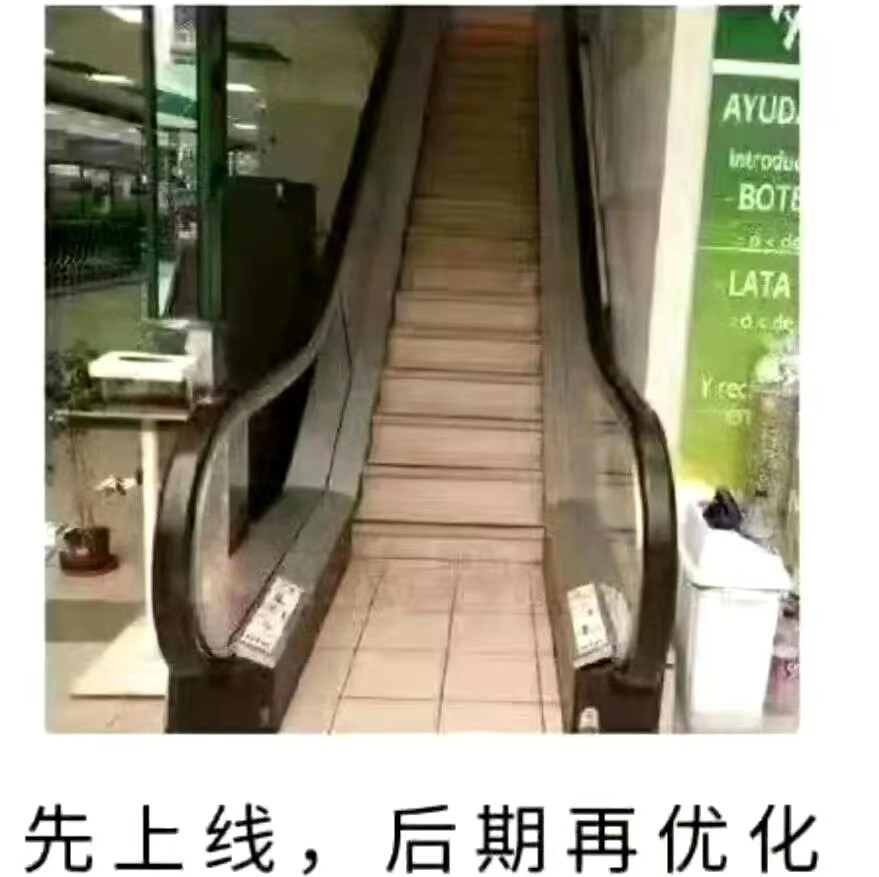
\includegraphics[scale=0.6]{xianshangxian_zaiyouhua.jpg}
\end{figure}


\indent
这本东西起源于我自己的各种杂七杂八的笔记,我想把它们整理起来,系统化并且数字化,于是在大三上学期有了一个基本的雏形.
后来我想,为什么不干脆再扩充一些,搞个讲义出来呢?这样还可以给别人看,多棒.
于是大三寒假我开始慢慢扩充这本讲义,也许会一直写下去,直到哪天我没了兴趣.

\begin{figure}[H]%插入题目的图片
  \centering
  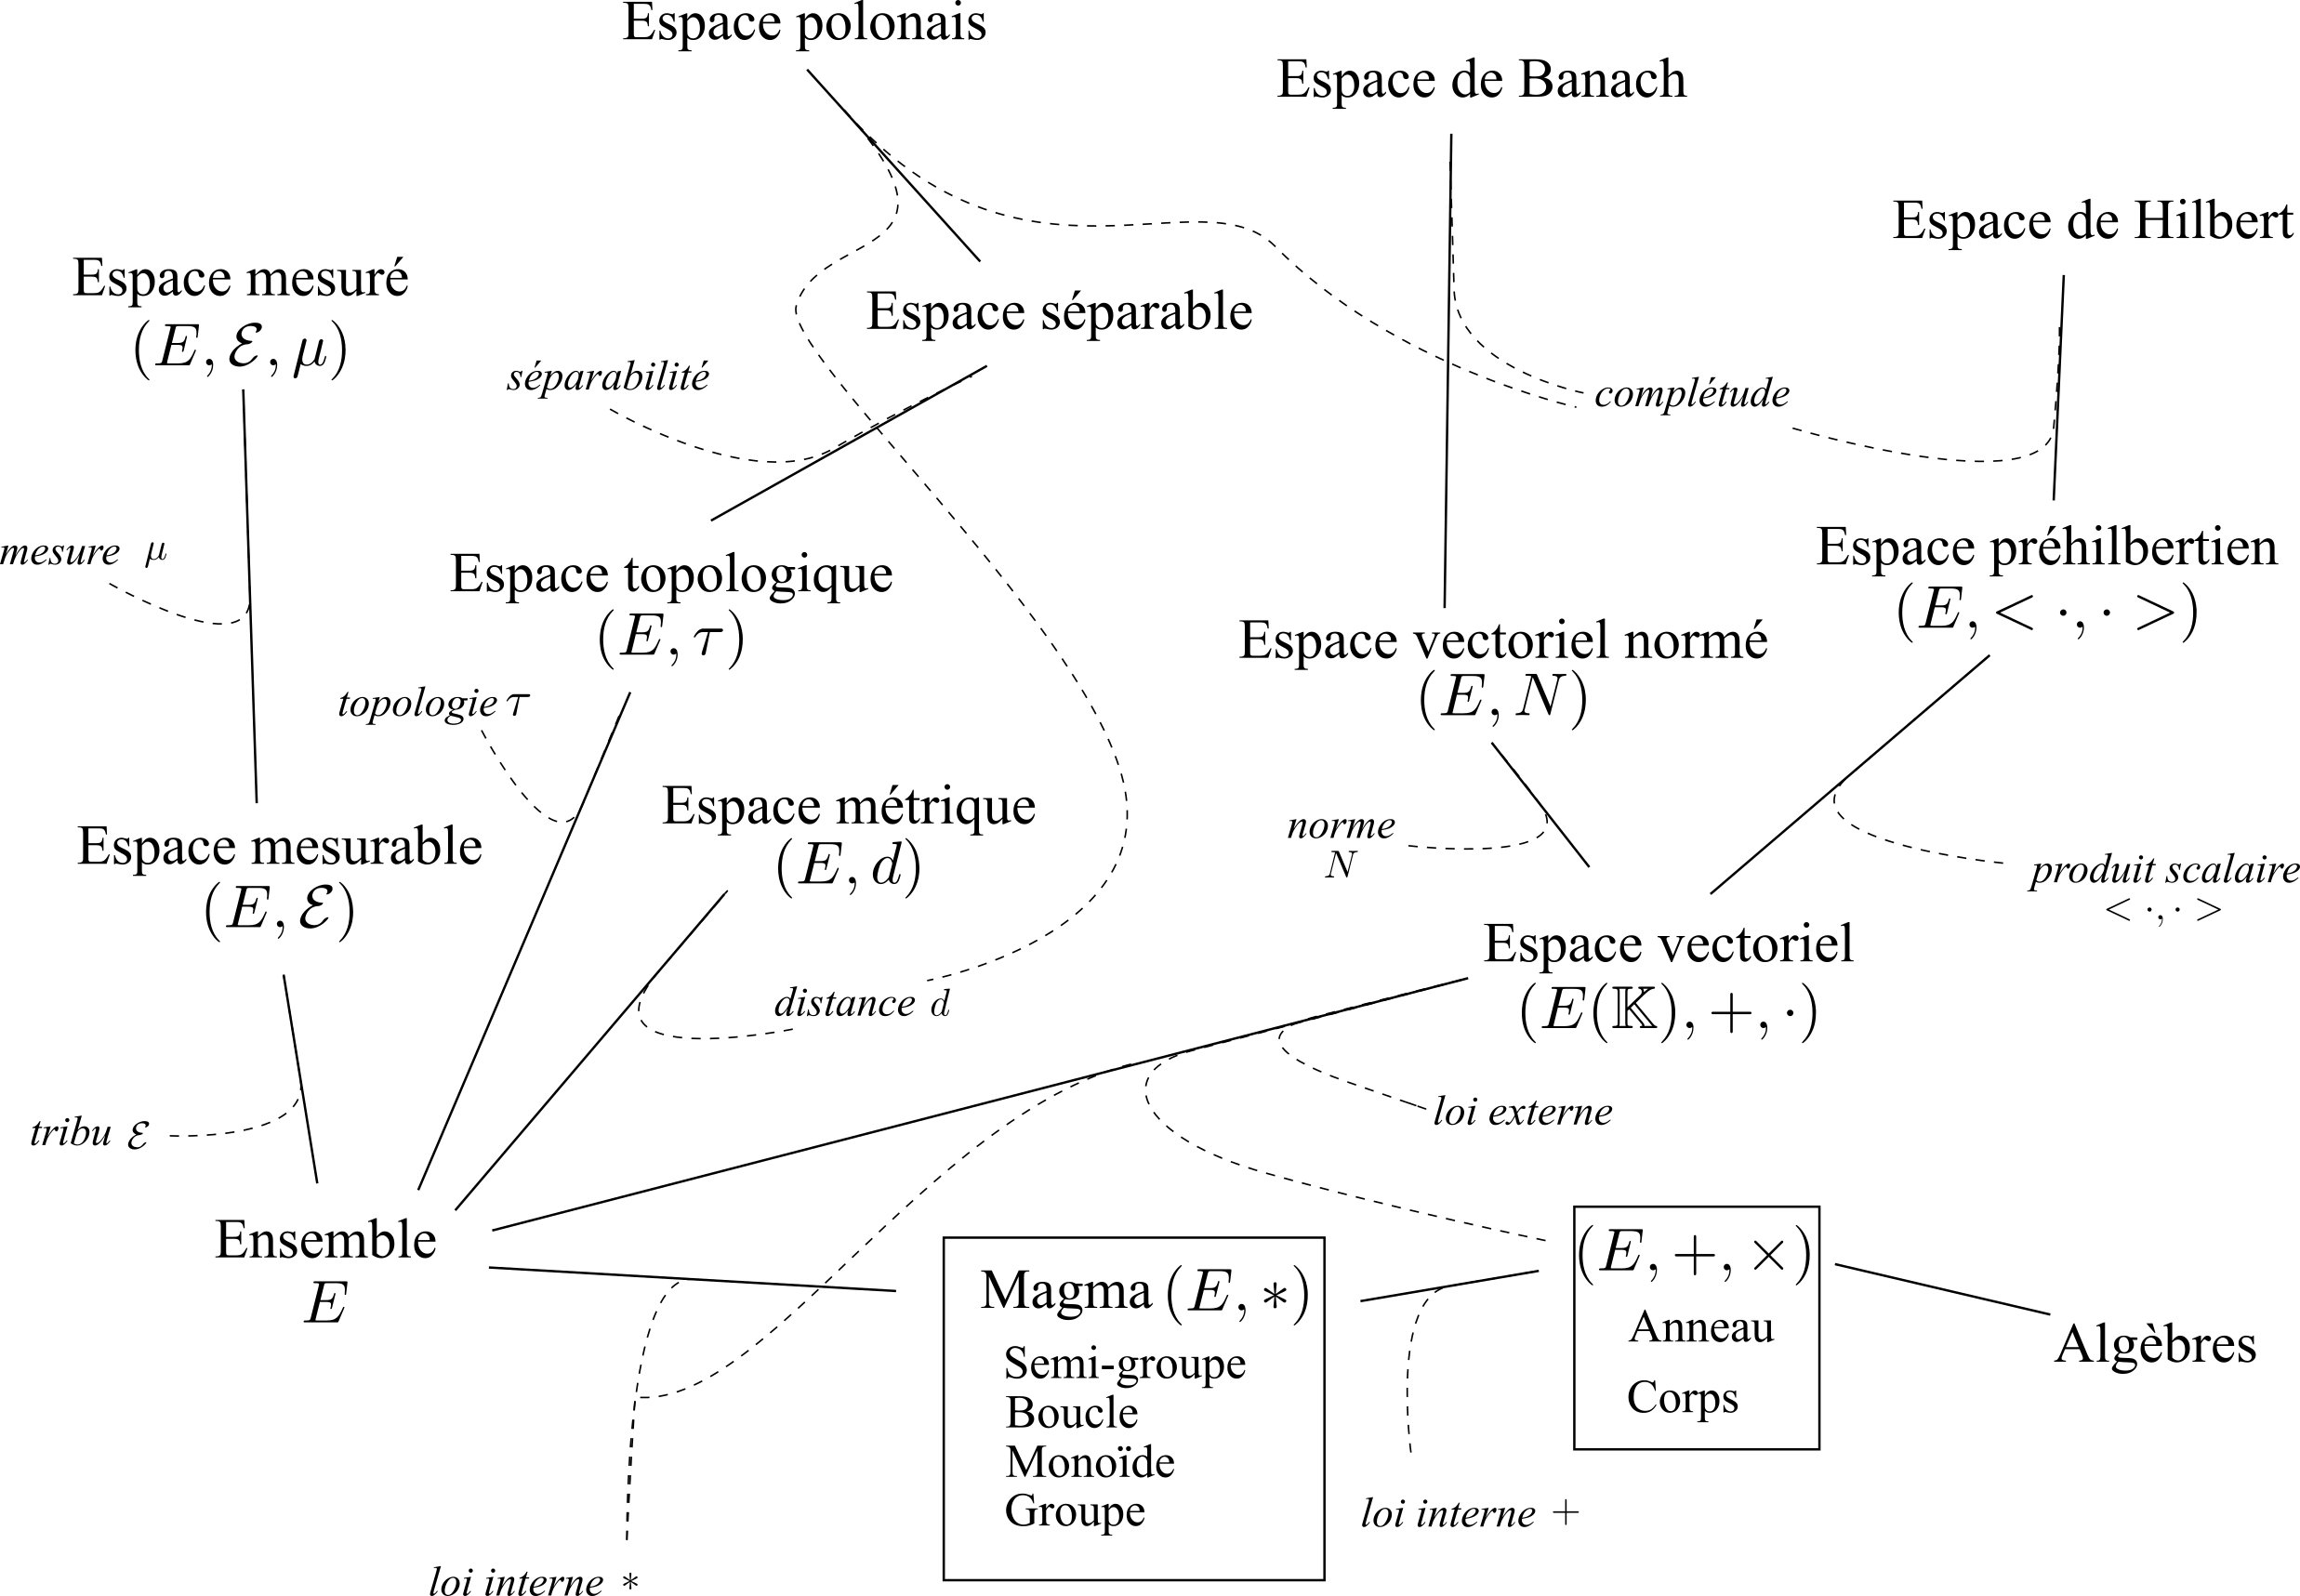
\includegraphics[scale=0.5]{abstract.png}
  \caption{数学分析部分知识关系(图源自法语wiki)}
  \label{myref:abstract}
\end{figure}

知识是网状的,而书是线性的.特别是,当你用维基百科对比一本教科书的时候,最能体现这个观点.
书的线性内容决定了作者不可能一开始就默认读者知道某个概念的所有相关概念,所以延伸性和复杂性都远远不够;而对于维基百科,就会有各种延申,每一个不知道的概念都可以点进去学习,就像是查字典.
因此任何一本书的内容都是一个线性的体系,后面的内容承接前面的内容,体现不了知识的复杂性,书的顺序也只是作者认为合理的顺序,不一定代表最适合每个读者的顺序.
所以我给出的也只是我觉得可以说得通的顺序.事实上存在大量平行的内容,相互之间怎么排列都可以.
(待更新)

本讲义大概有两种内容,即课程内容和课程的前置与延申内容.
对于课程内容,还是希望上课好好听讲,因此写的东西仅仅作为一个参考预习、复习的样例,说白了就是让你知道你学的是什么.方便读者在详细的不懂得地方可以多问老师或者自己找课程学习;
对于课外的内容,由于学院本身对于数学的要求不高,所以也只是介绍一下,并不深入.有兴趣的自己去找课程和书就行.这部分更像是一个简介,让你知道还有什么是我们没有学的,其中有哪些学一下更好.
对于讲义的参考资料,欢迎大家自己去找来看,这些东西远远比我写的精彩.我做的一点微小的工作其实就是把这些精华筛选一下,挑出我们课程用得上的东西,然后排列组合罢了.\\

\noindent
附部分讲义的参考资料与推荐阅读的资料:\\
出版物:
\begin{itemize}
  \item Proofs from THE BOOK,Martin Aigner \& Günter M. Ziegler,Springer
  \item The Princeton Companion to Applied Mathematics,Nicholas J. Higham,Princeton University Press
  \item Calcul Différentiel et Équations Différentielles,Sylvie Benzoni-Gavage,DUNOD
  \item Calcul Différentiel et Calcul Intégral,Noureddine El Jaouhari,DUNOD
  \item Topologie générale et espaces normés,Nawfal El Hage Hassan,DUNOD
  \item Les Maths en Physique,Jean-Pierre Provost et Gérard vallée,DUNOD
  \item Analyse Fonctionnelle et Théorie des Opérateurs,Josette Charles et al.,DUNOD
  \item Mathématiques pour l'Ingénieur,Yves Leroyer et Patrice Tesson,DUNOD
  \item Analyse Complexe pour la Licence 3,Patrice Tauvel,DUNOD
  \item Calcul Différentiel,Gilles CHARRON et Pierre PARENT,Cheneliere Education
  \item Algèbre Linéaire, Algèbre Bilinéaire,Mohamed Houimdi,Ellipses
  \item Éléments d'analyse et d'algèbre(et de théorie des nombres),Pierre Colmez,les Éditions de l'École Polytechnique
  \item Graduate Texts in Mathematics 73,S.Axler et al.,Springer
  \item Précis d'analyse réelle,Vilmos KOMORNIK, Ellipses
  \item The Princeton Companion to Applied Mathematics,Nicholas j. Higham,Princeton University Press
  \item Vector Calculus, Linear Algebra and Diffrerenial Forms: A Unified Approach,John H, Hubbard,Matrix Editions
  \item Théorie Analytique de la Chaleur,Jean-Baptiste Joseph Fourier,CAMBRIDGE
  \item Organic Chemistry,Jonathan Clayden te al.,OXFORD
  \item Chemical Applications of Symmetry and Group Theory,Rakshit Ameta \& Suresh C.Ameta,CRC Press
  \item Chemical Applications of Group Theory, F. Albert Cotton,
  \item 微积分和数学分析引论,R.科朗 \& F.约翰,科学出版社
  \item 数学分析原理,Walter Rudin,机械工业出版社
  \item 普林斯顿微积分读本,Adrian Banner,人民邮电出版社
  \item 普林斯顿线性代数读本,拉菲·格林贝格,人民邮电出版社
  \item 普林斯顿概率论读本,史蒂文·J.米勒,人民邮电出版社
  \item 代数学教程,R·戈德门特,高等教育出版社
  \item 陶哲轩实分析,陶哲轩,人民邮电出版社
  \item 数学分析中的问题和反例,汪林,高等教育出版社
  \item 拓扑空间与线性拓扑空间中的反例,汪林,高等教育出版社
  \item 实分析中的反例,汪林,高等教育出版社
  \item 泛函分析中的反例,汪林,高等教育出版社
  \item 拓扑学教程,G·肖盖,高等教育出版社
  \item 抽象代数基础,丘维声,高等教育出版社
  \item 代数的历史,约翰·德比希尔,人民邮电出版社
  \item 概率论基础教程,Sheldon M. Ross,机械工业出版社
  \item 数学建模,Frank R. Giordano etc.,机械工业出版社
  \item 数学分析,B.A.卓里奇,高等教育出版社
\end{itemize}
网络资料:
\begin{itemize}
  \item \href{https://space.bilibili.com/391930545}{Maki的完美算术教室},以及\href{https://www.maki-math.com/#/}{Maki-math.com}
  \item \href{https://www.zhihu.com/people/xavir-79/posts}{xavir}
  \item \href{https://space.bilibili.com/1632276842}{Ayumu爱讲数学}
  \item \href{https://space.bilibili.com/29977151}{James课后习题解答}
  \item \href{https://space.bilibili.com/6073855}{Druid小德}
  \item \href{https://space.bilibili.com/3156848}{kumiko想要学分析}
  \item \href{https://space.bilibili.com/586867165}{柚柚柚子235}
  \item \href{https://space.bilibili.com/20883932}{轩兔}
  \item \href{https://space.bilibili.com/184538069}{castelu}
  \item \href{https://space.bilibili.com/88461692}{3Blue1Brown}
  \item \href{https://space.bilibili.com/415941398}{返朴科普}
  \item \href{https://zh.wikipedia.org/wiki/Wikipedia:%E9%A6%96%E9%A1%B5}{中文}、\href{https://en.wikipedia.org/wiki/Main_Page}{英语}和\href{https://fr.wikipedia.org/wiki/Wikip%C3%A9dia:Accueil_principal}{法语}的维基百科
\end{itemize}


~\\
\begin{flushright}
    \begin{tabular}{c}
        Augustin\\
        2022年12月31日
    \end{tabular}
\end{flushright}


\newpage
\begin{center}
  \begin{figure}[H]%插入题目的图片
    \centering
    
\includegraphics[scale=0.3]{theo_math.png}
  \end{figure}
  \Huge\textbf{版本更新说明}
\end{center}~\


\noindent
\textbf{更新内容:}
\begin{itemize}
  %\item 删除了一些一年内不太可能学到的内容
  \item 应用部分内容调整
  %\item 把概率相关的内容调整进入应用
  \item 添加了一些法语原文表述
  \item 重写了逻辑
  \item 重写了可数性
\end{itemize}

\noindent
\textbf{计划中的更新:}
\begin{itemize}
  \item 尝试加入更多图片.等假期慢慢搞.
  \item 尝试给出一些习题.
  \item 补充证明.
  \item 对于重要的概念,补充完法语原文
  \item 对代数部分内容重新整理
  \item Bonus.
  \item 规范符号$\rightarrow,\mapsto $等等.
\end{itemize}




\newpage
\pagenumbering{Roman}
\setcounter{page}{1}
\tableofcontents

\newpage
\setcounter{page}{1}
\pagenumbering{arabic}

\part{基础知识\\ Notions Élémentaires}
\chapter{逻辑与证明\\ Logique et Démonstration}
  这一章内容是数学最基本的、最底层的概念.对于绝大多数阅读这份讲义的人而言,前几节的东西都已经学习过了,或者显而易见的.
  但这并不意味着这一章的内容就很好写,或者很好讲明白.也因此,为了保持知识的丰富度和连贯性,有许多还没在本讲义里被严格定义,但是其实已经学过的知识会出现在本章(后面也是).
  对于绝大多数这类情况,并不存在阅读障碍.但是,如果你发现有什么地方不太对劲,或者有什么地方不太懂,欢迎联系我,我会尽快修改.\\


  这一章(以及后面的章节里)有相当多的符号,关于这些符号的采用和相关的历史,欢迎参阅\url{https://jeff560.tripod.com/set.html}.
  \section{基本逻辑 Basic Logique}
  
  \subsection{命题逻辑 Logique propositionnelle}
  命题(Proposition)是一个陈述句所表达的判断,不是真的就是假的.例如“我不懂数学”就是一个命题.当然,在本讲义中,带有Proposition节标题的内容都被认为是真的.
  \subsubsection{逻辑析取:或  la disjonction: ou}
  定义符号 $\lor $ 表示两个命题的逻辑析取.对于命题$p,q,\text{若}p$是真的或者$q$是真的,则$p\lor q$是真的.
  \subsubsection{逻辑合取:与  la conjonction: et }
  定义符号 $\land  $ 表示两个命题的逻辑合取.对于命题$p,q,\text{若}p$和$q$都真的,则$p\land q$是真的.
  \subsubsection{逻辑否定:非  la négation: non}
  定义符号 $\lnot $ 表示命题的逻辑否定.若命题$p$是真的,则$\lnot(p)$是假的.
  \subsubsection{逻辑蕴含 l'implication}
  定义符号 $\Rightarrow$ 表示两个命题的逻辑蕴含.对于命题$p,q$,将$p\lor(\lnot q)$记为$q\Rightarrow p$.
  表示若$q$是真的则$p$也是真的.注意,如果$p,q$都不是真的,$q\Rightarrow p$也是真的.
  \subsubsection{逻辑等价 l'équivalence}
  定义符号 $\Rightarrow$ 表示两个命题的逻辑等价.对于命题$p,q$,将$(p\Rightarrow q)\land (q\Rightarrow p)$记为$p\Leftrightarrow q$.
  称作p等价于q.
  \subsection{逻辑公理 Axiomes de la logique}
  公理被认为是清晰地为真的命题.以下给出逻辑的四条公理.
  \subsubsection{$AL_1$}
  $(p\lor p)\Rightarrow p$是真的.这说明,如果$(p\lor p)$为真,则$p$为真.
  \subsubsection{$AL_2$}
  $p\Rightarrow (p\lor q)$是真的.这说明,如果$p$为真,则$(p\lor q)$为真.
  \subsubsection{$AL_3$}
  $(p\lor q)\Rightarrow (q\lor p)$是真的.这说明,如果$(p\lor q)$为真,则$(q\lor p)$为真.
  \subsubsection{$AL_4$}
  $(p\Rightarrow q)\Rightarrow [(p\lor r)\Rightarrow(q\lor r)]$是真的.
  \subsection{De Morgan定律 Lois de De Morgan}\index{De Morgan 定律}
  数学家Augustus De Morgan发现了命题逻辑中存在着如下关系:
  \begin{itemize}
    \item $\lnot (p\wedge q)\equiv (\lnot p)\vee (\lnot q) $
    \item $\lnot (p\vee q)\equiv (\lnot p)\wedge (\lnot q) $
  \end{itemize}称为De Morgan定律,又叫对偶律.

  \subsection{量词 Quantificateur}
  \subsubsection{全称量词 Quantification Universelle}
  全称量词$\forall$表示“对所有的(pour tout)”.由Gerhard Gentzen首先于1933年使用,将德语“一切(alle)”的首字母倒过来.

  \subsubsection{存在量词 Quantification Existentielle}
  存在量词$\exists$表示“存在(il existe)”.由Giuseppe Peano首先于1897年使用,后被Bertrand Arthur William Russell正式用于表示“存在”.
  此外,存在量词$\exists !$表示“有且仅有唯一的(il existe et seul)”.

  \section{证明 Démonstration}
  给定命题$p$,现在并不清楚命题是真是假.如果我们想要命题为真,就需要从逻辑上证明.同理,如果想要为假,也要从逻辑上证伪.这些都属于证明.
  \subsection{逻辑变换 Transformations logiques}
  蕴含命题$p\Rightarrow q$,全称命题$\forall x,p(x)$和存在命题$\exists x,q(x)$有如下的逻辑变换:
  \subsubsection{逆命题 Implication Réciproque}
  蕴含命题$p\Rightarrow q$的逆命题为$q\Rightarrow p$,逆命题不受量词影响,即$\forall x,p(x)\Rightarrow q(x)$的逆命题为$\forall x,q(x)\Rightarrow p(x)$.
  \subsubsection{否命题 }
  蕴含命题$p\Rightarrow q$的否命题为$\lnot p\Rightarrow \lnot q$.
  全称命题$\forall x,p(x)$的否命题为$\exists x,\lnot p(x)$,
  存在命题$\exists x,q(x)$的否命题为$\forall x,\lnot q(x)$.
  \subsubsection{逆否命题 Proposition Contraposée}
  蕴含命题$p\Rightarrow q$的逆否命题为$\lnot q\Rightarrow \lnot p$.逆否命题与原命题等价.
  \subsection{三段论 Syllogisme}
  三段论是涉及三个命题的论证,形式如$[(A\Rightarrow B)\land (B\Rightarrow C)]\Rightarrow (A\Rightarrow C)$.
  一般而言,一个三段论分为大前提(Prémisse majeure),小前提(Prémisse mineure)和结论(Conclusion)三段.
  大前提是某种普遍性质的规律,小前提是一个特殊陈述,结论就是我们要证明的内容.
  例如要证明114是偶数,我们需要:\begin{itemize}
    \item 大前提:能整除2的数是偶数.
    \item 小前提:114能整除2.
    \item 结论:114是整数.
  \end{itemize}
  三段论的每段共有四种含义,分别为:
  \begin{itemize}
    \item A:$\forall s,p(s)$.例如:所有自然数都是实数.
    \item E:$\forall s,\lnot p(s)$.例如:所有自然数都不是负数.
    \item I:$\exists s,p(s)$.例如:存在实数是自然数.
    \item O:$\exists s,\lnot p(s)$.例如:存在实数不是自然数.
  \end{itemize}
  因此一个三段论可以被简写称诸如AAA或者AEO这样的形式,共计256种!然而只有24种是有效的.在这里我就不一一列出了,有兴趣的读者自行查阅相关内容.
  下面我们直接介绍具体的证明方法.当然,如果你能将证明方法与对应的三段论结构联系起来,那是非常棒的!

  \subsection{举例证明 Preuve par exemple}
  假设要证明命题“存在不可导连续函数”,我们只需要举出一个例子就行,比如绝对值函数$f(x)=|x|$.
  同理,证伪命题“所有连续函数都可导”也是这样.
  \subsection{逆否证明 Preuve par contraposée}
  逆否命题与原命题等价,因此只需证明或者证伪逆否命题,就能间接证明或证伪原命题.
  \subsection{反证法 Preuve par l'absurde}
  假设我们要证明命题A为真,我们可以假设$\lnot $A为真,然后推出一个矛盾的结果$\perp $,因此$\lnot $A为假,从而证明A为真.\\
  
  
  例如,我们要证明素数有无限个.采用反证法:$\lnot(\text{素数有无限个})\Rightarrow \text{素数有有限个} $.设全体素数组成的集合$\mathbb{P}=\{p_1,p_2,\dots,p_n\}$,
  设$n=1+\prod _{i=1}^{n}p_1$,显然$n\notin \mathbb{P}$.若\n 是素数,则我们得到了一个不属于全体素数集合的素数,这显然矛盾.若\n 不是素数,对其质因数分解,选择任意一个质因子$m$.
  若$m\in \mathbb{P}$,则$m$既是$1+\prod _{i=1}^{n}p_1$的因子,又是$\prod _{i=1}^{n}p_1$的因子,因此必须是两者之差1的因子,也就是1.因此$n=m\cdot 1$,\n 显然是素数,
  所以我们又得到了矛盾的结果.所以,只能是我们的前提“素数有有限个”是错的,故素数有无限个.
  \subsection{归纳法 Preuve par récurrence}
  
  \subsection{分类讨论 Preuve par cas}



  
  更多关于证明的例子和技巧,可以参阅roofs from THE BOOK这本书(中文名叫《数学天书中的证明》),其涵盖了数论、几何、分析、组合数学和图论的许多精美的证明.

  \section{严格逻辑公式 Formules strictes}
  通过以上的逻辑符号和公理,加上两个用于判断的符号 $\perp $ 表示"假"和 $\top $ 表示"真",我们可以构造出一些严格逻辑公式.
  \subsection{Définition: Formule stricte}
  严格逻辑公式的定义实际上是一种归纳法.
  \begin{enumerate}
    \item $\perp $ 和 $\top $ 是严格逻辑公式.
    \item 任意的变量都是严格逻辑公式.
    \item 对任意严格逻辑公式$A$, $\lnot A$也是严格逻辑公式.
    \item 对任意两个严格逻辑公式$A$和$B$, $(A\land B)$,$(A\lor B)$,$(A\Rightarrow B)$,$(A\Leftrightarrow B)$也是严格逻辑公式.
  \end{enumerate}
  在一些推理中,利用$\circ$代表$\land,\lor,\Rightarrow,\Leftrightarrow$中的任意一个,并将 formule stricte 简称为逻辑公式 formule.
  此外,对于除了$\perp $和$\top $以外的逻辑公式,我们称其为可分解的(décomposable).
  \subsubsection{Exemple}
  $(a\lor(\lnot b\land c))$是逻辑公式,但是$a\lor(\lnot b\land c)$和$(a\lor(\lnot( b)\land c))$不是.
  \subsection{Définition: 子公式 Sous-formule stricte}
  称(严格)公式 $A$ 的任何因子为$A$的子公式.例如$(\lnot b\land c)$是$(a\lor(\lnot b\land c))$的子公式.
  \subsection{Définition: 公式的长度 Longueur d'une formule}
  公式 $A$ 的长度是用于编写 $A$ 的符号数量,用 $l(A)$ 表示.
  如果我们将公式视为用词汇表中的元素构成的词,其中的元素包括常量、变量、括号和连接符.
  则在这个词汇表上的一个词是该词汇表中元素的一个序列,而该词的长度是该序列的长度.
  例如$A=(a\land b)$,$B=(A\lor \lnot A)$,则$l(A)=5,\,l(B)=4+5+5=14$.
  \subsection{Définition: 公式的前缀 Préfixe d'une formule}
  对任意公式$A$,其前缀(préfixe)是从该公式的开头一直延伸到某个位置的部分.
  这个位置可以是一个特定的字符,一个操作符或一个括号,用来截断公式的前缀.
  例如$($和$(a$都是$A=(a\land b)$的前缀.但是$)$或者$b)$不是.
  此外,对于长度严格小于$A$的前缀,我们称其为严格前缀(préfixe strict).
  \subsection{括号的平衡  Équilibre des parenthèses}
  任何公式都具有相等数量的开括号"$($"和闭括号"$)$".可直接由定义和归纳法得到.
  \subsection{括号的关联 Relation entre les parenthèses}
  任何公式的前缀都具有至少与闭括号相等数量的开括号.
  \subsubsection{Démonstration}
  首先假设对于任意长度小于$n$的公式,该定理都成立。接着假设$l(A)=n$.
  \begin{enumerate}
    \item 若$A$是一个变量或者常量,则$A$没有括号,因此该定理成立.
    \item 若$A=\lnot B$,则$A$的前缀要么是空的或者$\lnot$,要么是$\lnot$跟随$B$的前缀,而$l(B)<n$,因此该定理成立.
    \item 若$A=(B\circ C)$,则$A$的前缀要么是空的或者开括号,要么是开括号跟随$B$的前缀,要么是开括号跟随$B\circ$和$C$的前缀.根据以上结论,都满足该定理.
  \end{enumerate}
  因此,如果引理对于所有长度小于$n$的公式都成立,那么它也对于长度为$n$的任何公式成立。
  通过归纳法,我们可以得出它对于任何长度的公式都成立。
  这个证明证明了数学逻辑中公式的括号平衡性质。
  \subsection{Définition: 公式的大小 Taille d'une formule}
  对公式$A$定义$|A|$为:
  \begin{itemize}
    \item 若$A$是$\perp$或$\bot$,则$|A|=0$.
    \item 若$A$是变量,则$|A|=0$.(?)
    \item $|\lnot A|=1+|A|$.
    \item $|A\circ B|=1+|A|+|B|$.
  \end{itemize}
  \subsection{严格前缀引理 Lemme des préfixes stricts}
  任何公式的严格前缀不是一个公式.\\
  Tout préfixe strict d'une formule n'est pas une formule.
  \subsubsection{Démonstration}
  仍然采用归纳法.对于基本情况$|A|=0$,$A$要么是变量要么是常量,其严格前缀只能是空的,故不是公式.
  假设对于任意长度小于$n$的公式,该定理都成立。接着假设$|A|=n$.

  若$A=\lnot B$,则$A$的严格前缀要么是空的或者$\lnot$,要么是$\lnot$跟随$B$的严格前缀,而$|B|<n$,因此该定理成立.

  若$A=(B\circ C)$,假设$A$有一个为公式的严格前缀$A_0=(B\circ C_0)$,其中$C_0$是$C$的前缀.
  为了保持公式的开括号与闭括号数量一致,我们必须有$C_0=C$.因此$A_0=A$,与严格前缀矛盾.因此该定理成立.
  \subsection{Proposition}\label{myref:sixuanyi}
  对于任何公式$A$,其有且仅有可能为以下形式之一:
  \begin{itemize}
    \item $A$是一个变量
    \item $A$是一个常量
    \item $A=\lnot B$,其中$B$是一个公式,且$A$是唯一的
    \item $A=(B\circ C)$,其中$B,C$是公式,且$A$是唯一的
  \end{itemize}
  \subsubsection{Démonstration}
  事实上我们只需证明最后一种形式.同样可以假设$A=(B\circ C)=(B_0\circ C_0)$然后证明$B_0=B,\,C_0=C$.与之前没什么差别.
  \subsection{优先级 Priorité}
  在定义公式时,我们写了很多不必要的括号,例如每个公式周围的括号。现在,我们通过定义优先级为语法引入了更多的灵活性。
  同样利用归纳法定义具有优先级的公式(或称为优先级公式 formule à priorité):
  \begin{itemize}
    \item $\perp $ 和 $\top $ 是优先级公式.
    \item 任意的变量都是优先级公式.
    \item 对任意优先级公式$A$, $\lnot A$也是优先级公式.
    \item 对任意两个优先级公式$A$和$B$, $A\circ B$也是优先级公式.
    \item 对任意优先级公式$A$, $(A)$也是优先级公式.
  \end{itemize}
  例如$a\lor \lnot b\land c$是一个优先级公式,但它并不是公式.为了确保公式的唯一性,我们需要定义连接词的优先级顺序.
  \subsubsection{优先级顺序 Ordre de priorité des connecteurs}
  定义连接词的优先级顺序(由高到低)如下:
  \begin{enumerate}
    \item $\lnot$ 否定 la négation
    \item $\land$ 合取 la conjonction
    \item $\lor$  析取 la disjonction
    \item $\Rightarrow$ 蕴含 l'implication
    \item $\Leftrightarrow$ 等价 l'équivalence
  \end{enumerate}
  \subsubsection{Remarque}
  在相同优先级的情况下,左侧的连接词具有更高的优先级,但对于蕴含操作符,它是右结合的。
  我们将一个具有优先级的公式视为使用优先级可重新构建的公式的缩写。
  除非另有说明,我们将一个公式与其缩写视为相同。
  换句话说,我们关注的是一个公式的结构,而不是它的表面写法,这一结构通过"stricte"语法得以明确。
  因此,具有优先级的公式的大小将等于它所代表的严格公式的大小。
  \section{公式的意义 Sens des formules}
  在这一部分,我们将探讨如何确定一个公式的真假,而不依赖于为其变量分配的值。
  我们首先会定义逻辑连接词的含义,然后解释如何计算一个公式的真值,并展示紧凑性定理。
  最后,我们将介绍逻辑学中的基本概念定义,这些构成了逻辑学家们的通用语言。
  \subsection{连接词的真假 Valeur de vérité des connecteurs}
  通常用0表示值为假,用1表示值为真.这样,可以分别依据变量$x$和$y$的真假给出连接词的真假.
  \begin{table}[H]
    \centering
  \begin{tabular}{|c|c|c|c|c|c|c|}
    \hline
    $x$ & $y$ & $\neg x$ & $x \lor y$ & $x \land y$ & $x \Rightarrow y$ & $x \Leftrightarrow y$ \\\hline
    0 & 0 & 1 & 0 & 0 & 1 & 1 \\\hline
    0 & 1 & 1 & 1 & 0 & 1 & 0 \\\hline
    1 & 0 & 0 & 1 & 0 & 0 & 0 \\\hline
    1 & 1 & 0 & 1 & 1 & 1 & 1 \\\hline
    \end{tabular}
    \caption{连接词真值表 Table de vérité des connecteurs}
    \label{tab:connecteurs}
  \end{table}
  \subsection{公式的值 Valeur d'une formule}
  我们为公式中的每个变量分配一个来自集合 $B = \{0, 1\}$ 的值。
  公式的值通过将变量替换为它们的值并根据表\ref{tab:connecteurs}的操作来计算得到。
  然而,为了对公式进行推理,我们需要正式定义公式的值。
  \subsubsection{Définition: 赋值 Assignation}
  赋值是将公式中的所有变量映射到集合$B$中.

  Une assignation est une application de l'ensemble de toutes les variables d'une formule dans l'ensemble $B$.
  \subsubsection{Définition: 公式的值 Valeur d'une formule}
  对于一个公式$A$和一个赋值$v$,我们定义$A$在$v$下的值$[A]_v$如下,其中$A,B$是公式,$x$是变量,$v$是赋值.
  \begin{itemize}
    \item $[x]_v=v(x)$
    \item $[\bot]_v=1,\,[\perp]_v=0$
    \item $[\lnot A]_v=1-[A]_v$
    \item $[A\land b]_v=\max\{[A]_v,[B]_v \}$
    \item $[A\lor b]_v=\min\{[A]_v,[B]_v \}$
    \item $[A\Rightarrow b]_v=\begin{cases}
      1 & [A]_v=0\\
      [B]_v & [A]_v\neq 0
    \end{cases}$
    \item $[A\Leftrightarrow b]_v=\begin{cases}
      1 & [A]_v=[B]_v\\
      0 & [A]_v\neq [B]_v
    \end{cases}$
  \end{itemize}
  根据\prettyref{myref:sixuanyi}的结论,根据第14页的定理1.1.13,每个严格的公式都可以唯一分解为上述情况之一。
  这意味着将变量的赋值扩展到所有公式是一个从公式到B的映射。
  例如,对于四个公式 $A$、$A_0$、$B$ 和 $B_0$ 以及两个操作符 $\circ$ 和 $\circ_0$,
  如果 $(A\circ B)=(A_0\circ_0 B_0)$,则根据分解的唯一性,我们可以得出 $A=A_0$,$B=B_0$,$\circ=\circ_0$。
  因此,公式 $(A\circ B)$ 的值仅由值定义中的一行唯一确定。这表明公式的值仅与其包含的变量和结构有关,因此公式的计算以真值表的形式展示,如表\ref{tab:formes}所示.
  \begin{table}[ht]
    \centering
    \begin{tabular}{|c|c|c|c|c|c|c|}
      \hline
      $x$ & $y$ & $\neg x$ & $x\lor y$ & $x\land y$ & $x\Rightarrow y$ & $x\Leftrightarrow y$ \\\hline
      0 & 0 & 1 & 0 & 0 & 1 & 1 \\\hline
      0 & 1 & 1 & 1 & 0 & 1 & 0 \\\hline
      1 & 0 & 0 & 1 & 0 & 0 & 0 \\\hline
      1 & 1 & 0 & 1 & 1 & 1 & 1 \\
      \hline
    \end{tabular}
    \caption{公式真值表 Table de vérité des formules suivantes}
    \label{tab:formes}
  \end{table}

  \section{替换和取代 Substitution et remplacement}
  \section{标准形式 Formes normales}
  将一个公式转化为标准形式是将其转化为一个具有结构性质的等价公式的过程。
  我们引入了两种标准形式的概念:析取范式(Disjunctive Normal Form,DNF),用于突出模型,
  以及合取范式(Conjunctive Normal Form,CNF),用于展示反例。
  标准形式的定义需要引入文字(literal)、单项式(monomial)和子句(clause)的概念。


  \section{Boole代数 Algèbre de Boole}
  \section{Boole函数 Fonctions booléennes}
  \section{二进制决策图计算器 Binary Decision Diagram based Calculator}
\section{一阶逻辑 Logique du premier ordre}
  待修改






\chapter{集合\\ Ensembles}
  我们先从数学最基础的内容开始.前面这一部分内容在大一就已经讲过了,然而为了保持本讲义的连贯与严谨,不突兀地出现公理化集合论之类的东西,我们还是从头开始讲起.
\section{集合}
  为了便于你的理解,我们先给出集合的定义,并且顺着这些定义讨论,随后会在\prettyref{myref:gonglihua}这里把这些概念全部公理化,以求得到更深刻的理解.
  事实上,本讲义的许多内容,都是先讲个基础的概念,随后在某个内容里将这个概念公理化.
  \subsection{Définition}
  我们朴素地认为,一个集合就是将对象归类而分成为一个或数个形态各异的大小整体.
  一般来讲,集合是具有某种特性的事物的整体,或是一些确认对象的汇集.构成集合的事物或对象称为元素.集合的元素可以是任何东西.
  \subsection{集合的特性}
  集合具有以下几个特性:
  \begin{itemize}
    \item 无序性:一个集合中,每个元素的地位都是相同的,元素之间是无序的.\footnote{
      当然,如果我们在集合上定义了序,那么元素之间就可以按照序关系排序.但就集合本身的特性而言,元素之间没有必然的序.序关系将在后续阐明.
    }
    \item 互异性:一个集合中,每个元素只能出现一次,没有相同的元素出现.
    \item 确定性:给定一个集合,任给一个元素,该元素或者属于或者不属于该集合.\label{myref:quedingxing}
  \end{itemize}
  \subsection{索引族 Famille Indexée}
  若集合$I$中的每个元素,比如$i$,都对应着一个集合$A_i$,那么称$\mathscr{A}=\{A_i|i\in I\}$为集合$A$的索引族,集合$I$是其索引集.
  \subsubsection{Exemple}
  $A_n=\{1,14,n^2\}$,且有$\mathscr{A}=\{A_n|n\in [\![5,14]\!]\}$,则$\mathscr{A}$就是$A_n$的索引族,并且$\mathscr{A}=\{ \{1,14,25\}\{1,14,36\}\dots\{1,14,196\}\}$.
  \subsection{子集 Sous-ensemble}
  若集合$B$中的每个元素都属于集合$A$,则集合$B$是集合$A$的子集,则集合$A$是集合$B$的超集,记为$B\subseteq A$或者$A\supseteq B$.
  此外,若$B\subseteq A$且$A\subseteq B$,说明二者的元素相同,是同一个集合,记为$A=B$.
  \subsubsection{Proposition}
  对于任意集合$A$,有$\varnothing\subseteq A$.
  \subsection{幂集 Ensemble Puissance}
  对于任意集合$A$,其幂集为由该集合全部子集为元素构成的集合,记为$\mathcal{P},\mathcal{P}(A)=\{B| B\subseteq A\}$.
  有时也称之为ensemble des parties.

  \section{二元关系 Relation Binaire}
  \subsection{有序对 Couple}
  有序对是包含了两个元素的特殊的集合$(a,b)$.不同于一般的集合,有序对上的两个元素是有顺序的,
  分别被称为左投影和右投影,法语也叫première composante和deuxième composante.有序对的相等要求:
  $$
  (a_1,b_1)=(a_2,b_2)\Leftrightarrow (a_1=a_2)\land(b_1=b_2)
  $$有序对可以有其他有序对作为投影,所以有序对使得能够递归定义有序.
  例如,有序三元组 (a,b,c)可以定义为(a, (b,c)),一个对嵌入了另一个对.
  \subsection{Définition}
  二元关系将一个集合的元素与另一个集合的元素相关联.例如集合$X$和$Y$上的二元关系$\mathcal{R} $是一组新的有序对$(x,y)\text{组成的集合$\mathcal{G} $,其中}x\in X,y\in Y$.
  如果$(x,y)\in\mathcal{G}$,则称$x,y$有关系$\mathcal{R}$,记作$x\mathcal{R}y$或者$\mathcal{R}(x,y)$.
  \subsubsection{Exemple}
  $\mathbb{N}$上的大于关系$>$可以表示为$\{(a,b)|\exists r\in \mathbb{N},(a=b+r)\}$.记作$a>b$.
  \subsection{关系的性质}
  二元关系$R$可能拥有以下的某些性质:
  \subsubsection{自反性 Relation Réflexive}
  $\forall x\in X,(x,x)\in R$
  \subsubsection{非自反性 Relation Irréflexive}
  $\forall x\in X,(x,x)\notin R$
  \subsubsection{对称性 Relation Symétrique}
  $\forall x\in X,y\in Y,(x,y)\in R\Leftrightarrow(y,x)\in R$
  \subsubsection{反对称性 Relation Antisymétrique}
  $\forall x\in X,y\in Y,(x,y)\in R\land(y,x)\in R \Leftrightarrow x= y$
  \subsubsection{非对称性 Relation Asymétrique}
  $\forall x\in X,y\in Y,(x,y)\in R\Rightarrow (y,x)\notin R$
  \subsubsection{传递性  Relation Transitive}
  $\forall(x,y)\in R,\forall (y,z)\in R\Rightarrow(x,z)\in R$
  \subsection{等价关系 Relation d'Équivalence}
  若二元关系$\thicksim $满足自反性、传递性和对称性,则称其为等价关系,记作$a\thicksim b$.
  \subsubsection{Exemple}
  \begin{itemize}
    \item 集合的相等是等价关系.
    \item 三角形的相似关系和全等关系是等价关系.
    \item 温度相同是等价关系.
  \end{itemize}
  \subsubsection{等价类 Classe d'Équivalence}
  集合$E$上定义等价关系$\thicksim $,对$a\in E$,$a$的等价类为集合中所有与其等价的元素组成的集合$\{x|x\thicksim a\land x\in E\}$.
  
  \subsection{序关系 Relation d'Ordre}
  前文说过,集合上的元素本身是无序的,这意味着元素之间是平等的,无法比较的.
  例如给定集合$\{$2000CNY,3000USD,1919JPY,400EUR$\}$,我们并不知道四个元素分别意味着什么,也不知道他们的关系.现在给出 $Champion$ 断言: 2000CNY$\ge$3000USD.
  为什么可以这么说?显然,这说明存在某种“顺序”,这种“顺序”可以通过符号$\ge$来表示两个元素的关系.事实上,这就是一种序关系.下面我们分别介绍各种序关系.
  \subsubsection{全序关系 Relation d'Ordre Total}
  若集合$X$上的关系$\leq$满足自反性、传递性和反对称性,并且是“完全的(Totalité)”,也就是$\forall a\in X,\forall b\in X,(a\leq b)\lor(b\leq a)$.
  则称此关系为全序关系,或者非严格全序关系.\\
  
  相对应的,若集合$X$上的关系$<$定义为$a<b\Leftrightarrow \lnot(b\leq a)$,则称为严格全序关系(Ordre strict total).其满足反自反性、传递性和非对称性.
  \subsubsection{良序关系 Relation Bien Ordonné}
  若集合$X$上的全序关系$\leq$使得对任意子集$S,\exists i\in S,\forall s\in S,i\leq s$,则称此关系为良序关系.
  换句话说,任意子集有最小值的全序关系称为良序关系.

  \subsubsection{偏序关系 Relation d'Ordre Partiel}
  若集合$X$上的关系$\leq$满足自反性、传递性和反对称性,即不“完全”的全序关系被称为偏序关系.
  同理也有相对应的严格偏序关系$a<b$,使得$a<b\lor a=b\Rightarrow a\leq b$.
  \subsubsection{预序关系 Relation Préordre}
  若集合$X$上的关系$\preceq $满足自反性和传递性,则称之为一个预序关系.它既不一定是反对称的,也不一定是非对称的.
  预序关系有时也用$\lesssim $表示.将预序集的等价元素等同起来,可得到由该预序集所导出的偏序集.对称的预序就是等价关系.

\section{集合的运算 Opérateur}
  集合之间有以下几种常见的运算:
  \subsection{交集 Intersection}
  集合$A$和$B$的交集是两者共同包含的元素组成的集合,用符号$\cap$表示,即:
  $$
  A\cap B=\{x | (x\in A)\land (x\in B)\}
  $$


  \subsection{并集 Union/Réunion}
  与交集相对应,集合$A$和$B$的并集是两者包含的所有元素组成的集合,用符号$\cup$表示,即:
  $$
  A\cup B=\{x | (x\in A)\lor (x\in B)\}
  $$

  \subsection{Remarque: 交集与并集的性质 Propriété de l'lntersection et de l'union}
  \begin{itemize}
    \item 对于任意集合$A$,$A\cap A=A=A\cup A$.
    \item 交换律: $A\cap B=B\cap A,A\cup B=B\cup A$.
    \item 结合律: $(A\cap B)\cap C=A\cap (B\cap C),(A\cup B)\cup C=A\cup (B\cup C)$.
    \item $(A\cap B)\subseteq A\subseteq (A\cup B).$
    \item $A\subseteq B\Leftrightarrow A\cap B=A\Leftrightarrow A\cup B=B$.
  \end{itemize}
  \subsection{集合的分配律 Distributivité}
  有限个集合的交集与并集符合分配律,这是很重要的性质.对$n\in\mathbb{N}$:
  $$
  A\cup(\bigcap_{i=1}^{n}B_i)=\bigcap_{i=1}^{n}(A\cup B_i)
  $$
  $$
  A\cap(\bigcup_{i=1}^{n}B_i)=\bigcup_{i=1}^{n}(A\cap B_i)
  $$
  \subsection{补集 Complémentaire}
  集合$A$对于集合$B$的补集是属于$B$却不属于$A$的元素组成的集合,
  记为$ \complement _B^A$或者$A^C$:
  $$
  \complement _B^A=\{x\in B | x\notin A\}
  $$
  \subsection{差集 Différence}
  集合$A$对于集合$B$的差集是$A$中不属于$B$的元素组成的集合,可以被看作是补集的一种形式
  记为$A\backslash B$或者$A-B$:
  $$
    A\backslash B=\{x\in B | x\notin A\}
  $$
  \subsubsection{对称差 Différence symétrique}
  集合$A$和集合$B$的对称差是属于$B$或者属于$A$,却不同时属于两者的元素组成的集合,
  记为$A\Delta B$:
  $$
    A\Delta B=(A\cup B)\backslash (A\cap B)=(A\backslash B)\cup(B\backslash A)
  $$

  \subsection{笛卡尔积 Produit Cartésien}
  定义两个集合的笛卡尔(Descartes)积为其元素组成的有序对的集合,即:
  $$
  X\times Y=\{(x,y)|x\in X,y\in Y\}
  $$对于同一个集合对自身做笛卡尔积,我们采用幂的符号.如$A\times A=A^2$.

  \begin{figure}[H]
    \centering
    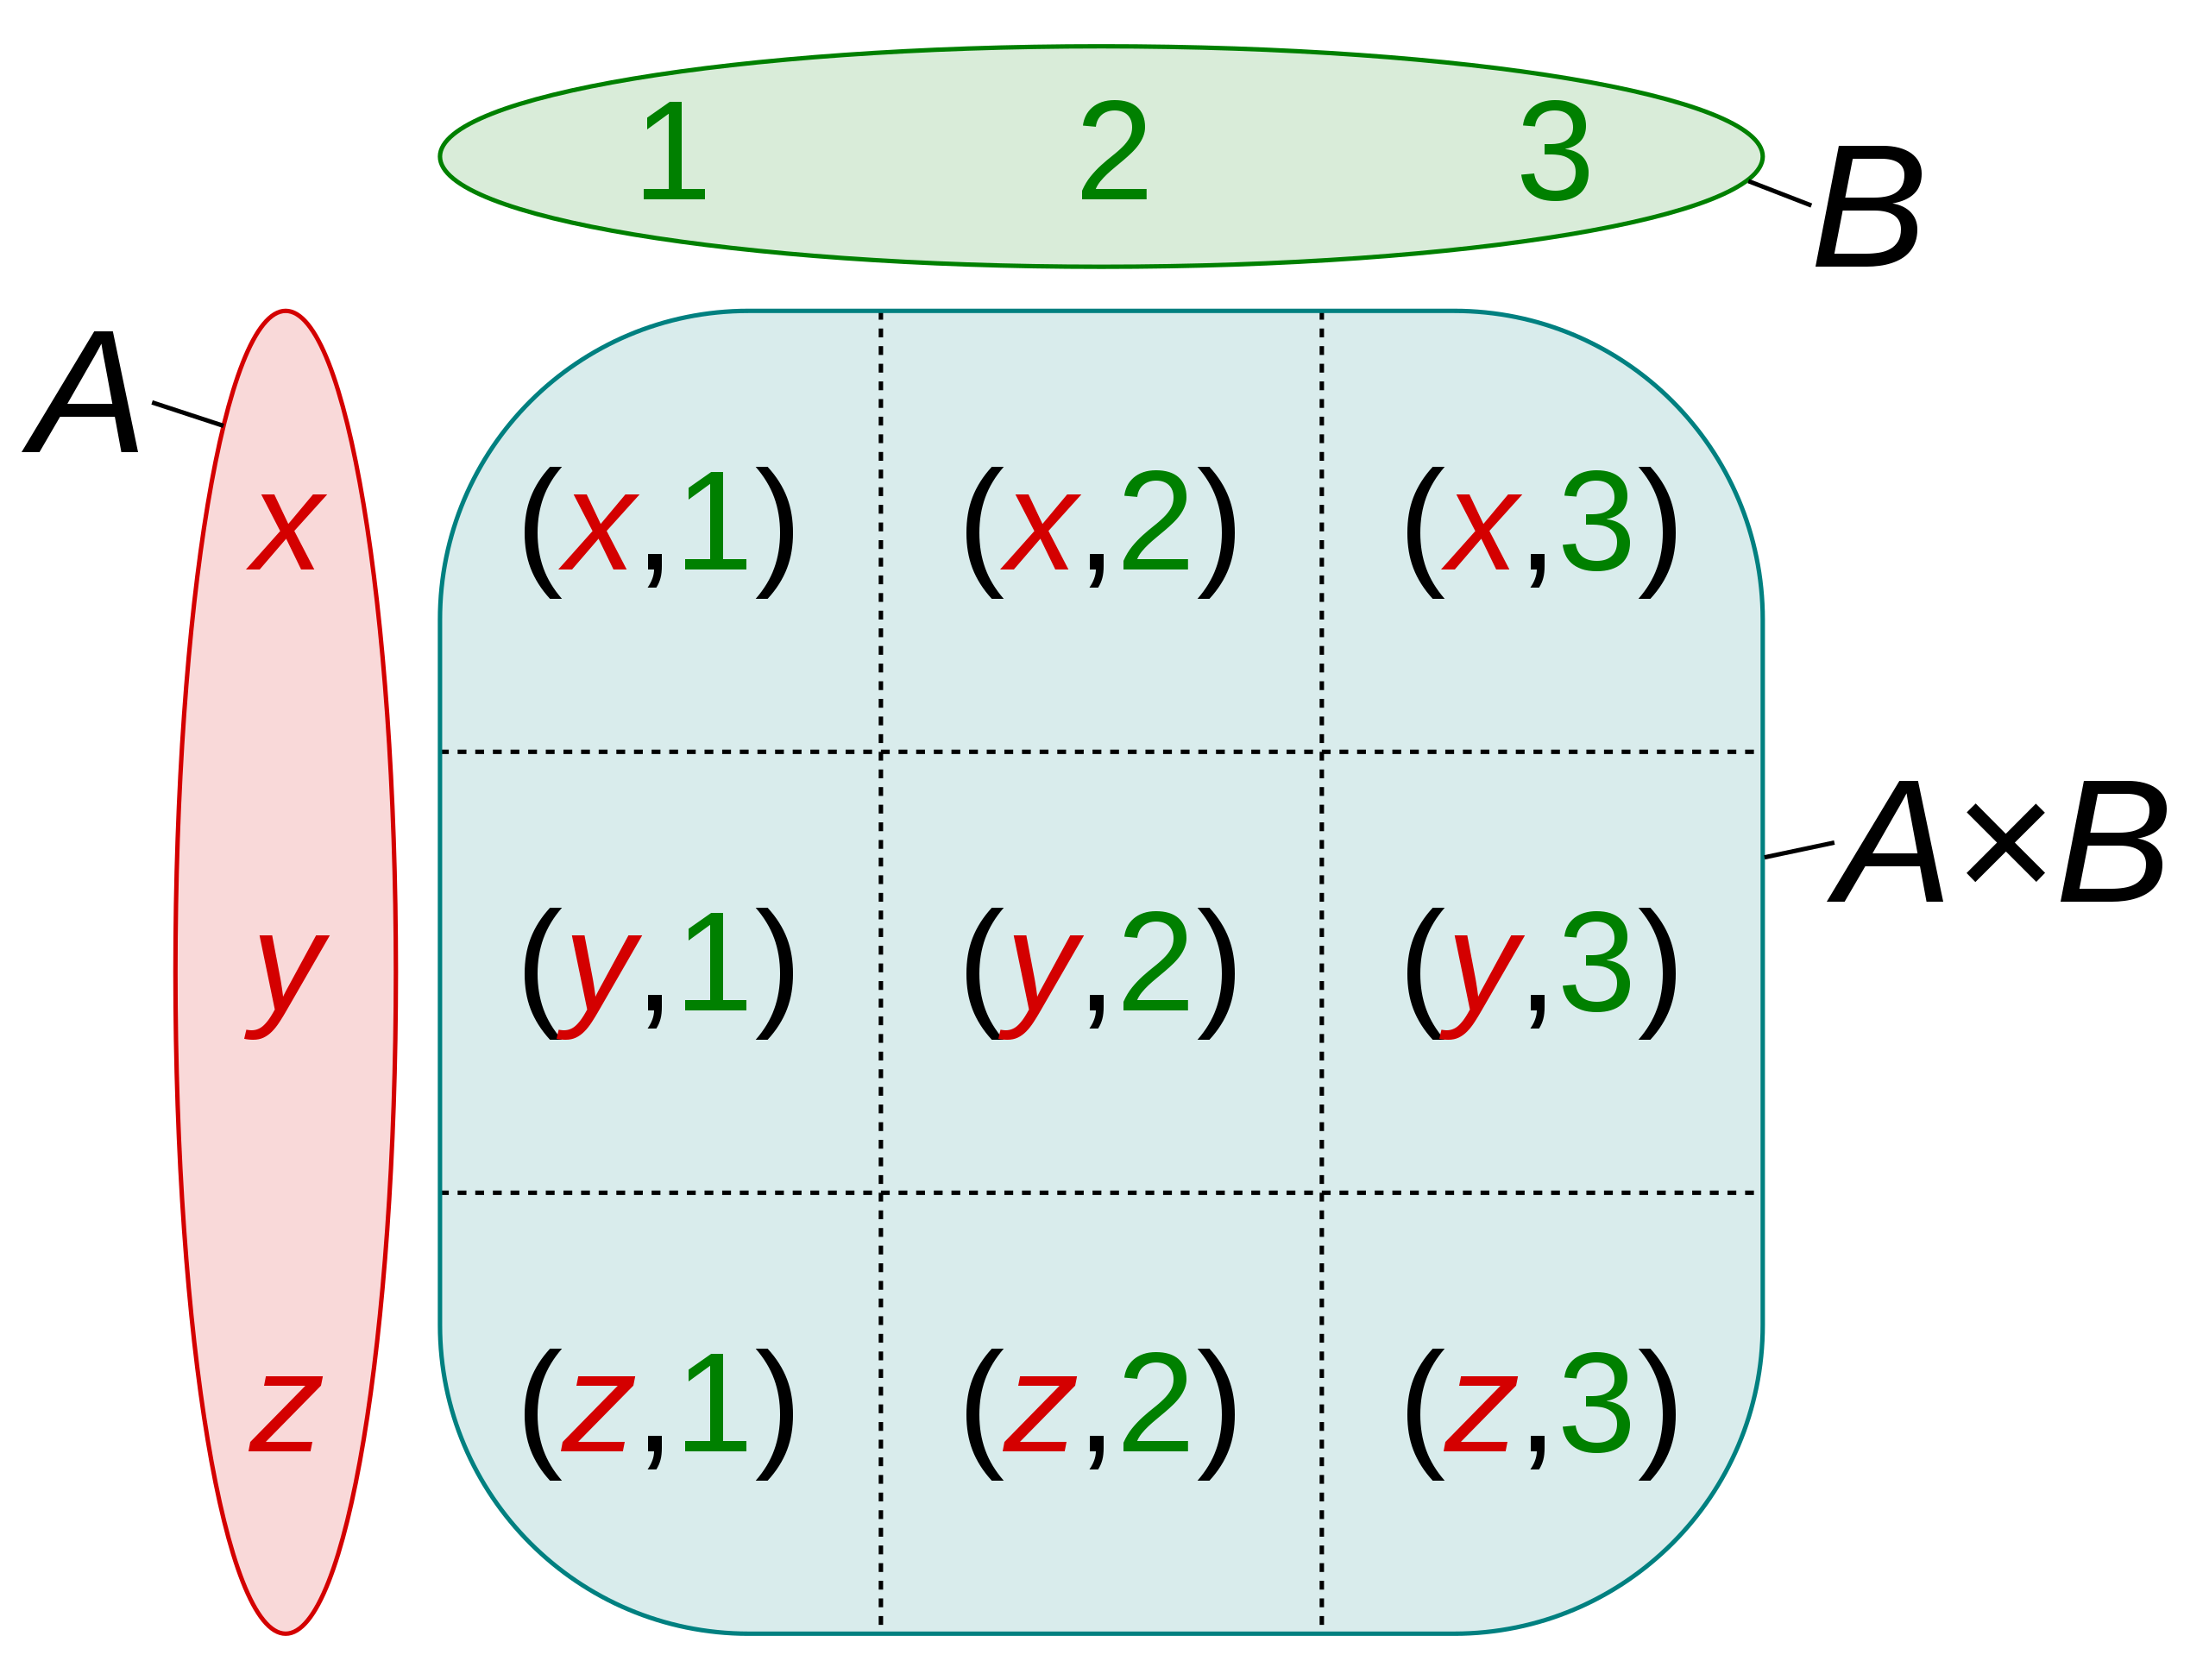
\includegraphics[scale=0.05]{Produit_Cartesien.png}
    \caption{Produit Cartésien(图源wiki)}
    \label{myref:Produit_Cartesien}
  \end{figure}
  \subsubsection{Exemple}
  我们最熟悉的平面直角坐标系就是$\R^2$.
  \subsection{De Morgan定律的集合形式}
  在集合论中,De Morgan定律表现为如下形式:
  \begin{itemize}
    \item $(A\cap B)^C=A^C\cup B^C $
    \item $(A\cup B)^C=A^C\cap B^C $
  \end{itemize}


  在经典命题逻辑的外延中,此二元性依然有效.即对于任意的逻辑运算符,我们都能找他它的对偶.
  这导致了基于传统逻辑的逻辑学的一个重要性质,即否定范式的存在性:如果其中否定仅出现在作用于公式中非逻辑的原子,任何公式都有它的等价公式.

  \section{公理化的集合论}\label{myref:gonglihua}
  主观意义上说,无论是ZF还是ZFC,在本讲义(或学院的课程)的“使用体验”上与原来朴素的直观的集合论没有什么区别,并且,有很多概念我们没有清晰.
  因此其实不必看懂这一章讲了什么,它不会影响你对后续章节内容的理解.
  \subsection{Russell悖论}
  现在,回头看看\prettyref{myref:quedingxing},尝试回答以下问题:\\
  设集合$A$是所有不属于自身的集合的集合,即$A=\{x | x\notin x\}$.那么请问$A$是否属于它自己?
  \begin{itemize}
    \item $A\in A$,说明$A$满足不满足其定义的不属于自身的性质,则$A\notin A$.
    \item $A\notin A$,说明$A$满足不属于自身的性质,则$A\in A$.
  \end{itemize}


  该悖论由数学家Bertrand Arthur William Russell提出,故称为Russell悖论.从经典逻辑的爆炸原理来看,任何命题都可以从矛盾中得到证明.
  因此,存在像Russell悖论这样的矛盾是灾难性的,因为如果任何公式可以被证明为真,它就破坏了真和假的含义.
  此外,由于集合论被视为所有其他数学分支公理化发展的基础,Russell悖论威胁到了整个数学的基础
  \footnote{
    其实除了Russell悖论,还有Burali-Forti悖论和Cantor悖论,但是相关的前置内容没有涉及,所以不放在这里讨论.
  },这激发了发展无矛盾的集合论的大量研究.
  \subsection{Zermelo-Fraenkel集合论:ZF公理体系}
  Zermelo-Fraenkel公理是众多集合论公理中的一员,也是对于不需要深入学习数学(特别是集合论)的我们最常见的公理体系.
  这套公理是二十世纪早期为了建构一个不会导致类似Russell悖论的矛盾的集合理论所提出的一个公理系统,简称为ZF公理.
  该公理体系包含以下公理:

    \subsubsection{外延性公理 Axiome d'extensionnalité}
      如果两个集合具有相同的元素则它们相等.\\\indent
      Si deux ensembles ont les mêmes éléments, alors ils sont égaux.
      $$
        \forall A\forall B,\forall x,(x\in A\Leftrightarrow x\in B)\Rightarrow A=B 
      $$

      \subsubsection{正规公理 Axiome de fondation/régularité}
      每个非空集合$X$都包含一个元素$y$,使得$X$和$y$不相交.\\\indent
      Tout ensemble $X$ non vide contient un élément $y$ tel que $X$ et $y$ sont des ensembles disjoints (qui n'ont aucun élément en commun).
      $$
        \forall X\neq \varnothing ,\exists y\in X,y\cap X=\varnothing 
      $$

      \subsubsection{分类公理 Schéma d'axiomes de compréhension/séparation}
      设$\mathbb{A}$为一个集合,且$P$为任一个描述$\mathbb{A}$内元素$x$的特征的性质,则存在$\mathbb{A}$的子集$A$包含$\mathbb{A}$内满足这个性质的$x$.\\\indent
      Pour tout ensemble $A$ et toute propriété $P$ exprimée dans le langage, il existe un ensemble dont les éléments sont les éléments de $A$ vérifiant $P$.
      $$
      \forall \{x| P(x) \}\subseteq \mathbb{A},\exists A\subseteq \mathbb{A},A=\{x| P(x)\}
      $$
      这样我们就可以定义空集了,例如对于集合$\mathbb{A},\varnothing =\{x|x\in\mathbb{Z}, x\neq x\}$.
      有时这也被称为空集公理(Axiome de l'ensemble vide).


      \subsubsection{配对公理 Axiome de la paire}
      若$X$和$Y$是集合,则存在一个集合包含$X$和$Y$. \\\indent
      Si $X$ et $Y$ sont deux ensembles, alors il existe un ensemble contenant $X$ et $Y$ et eux seuls comme éléments.
      $$
      \forall X\forall Y, \exists Z,X\in Z,y\in Z 
      $$

      \subsubsection{并集公理 Axiome de la réunion}
      对任一个集合$\mathcal{F}$,存在一个集合$A$,包含每个为$\mathcal{F}$的某个元素的元素的集合.\\\indent
      Pour tout ensemble $\mathcal{F}$, il existe un ensemble $A$ dont les éléments sont précisément les éléments des éléments de $\mathcal{F}$ et eux seuls.
      $$
      \forall \mathcal{F}\exists A,\forall F\subseteq\mathcal{F},\forall x\in F\Rightarrow x\in A 
      $$


      \subsubsection{替换公理 Schéma d'axiomes de remplacement}
      任何可定义函数下的集合的像也将落在集合内.\\\indent
      Pour tout ensemble $A$ et toute relation fonctionnelle $P$,formellement définie comme une proposition$P(x,y)$ et tel que $P(x,y)$ et $P(x,z)$ 
      impliquent que $y=z$, il existe un ensemble contenant précisément les images par $P$ des éléments de l'ensemble d'origine $A$.


      \subsubsection{无穷公理 Axiome de l'infini}
      存在包含无限多个元素的集合.\\\indent
      Il existe un ensemble $W$ dont $\varnothing$ est élément et tel que pour tout $X$ appartenant à $W$,$X\cup\{X\}$appartient aussi à $W$.
      $$
      \forall X,\, \exists \mathbb{W}, X\subseteq \mathbb{W}\Rightarrow X\cup \{X\}\subseteq \mathbb{W}
      $$


      \subsubsection{幂集公理 Axiome de l'ensemble des parties}
      对任一个集合$X$,存在一个集合$Y$为$X$的幂集的超集.\\\indent
      Pour tout ensemble $X$, il existe un ensemble dont les éléments sont précisément tous les sous-ensembles de $X$.
      $$
      \forall \mathbb{X},\exists \mathbb{Y},\forall X, X\subseteq \mathbb{X}\Rightarrow X\in\mathbb{Y}
      $$


      \subsubsection{良序定理 Théorème de Zermelo/du bon ordre}
      所有集合都可以被良序排序.\footnote{若给定前八个公理,就可以找到许多个和良序定理等价的叙述,例如选择公理.}\\\indent
      Tout ensemble peut être muni d'une structure de bon ordre.



  \subsection{选择公理 l'Axiome du choix: ZFC公理体系}
  对于所有的非空的索引族$(S_i)_{i\in I}$,存在一个索引集$(X_i)_{i\in I}$使得$\forall i\in I,X_i\in S_i $.
  它可以被理解为:给定任何非空集合的族,可以通过从每个集合中任意选择一个元素来构造一个新集合,即使其包含集合是无限的.\\

  对于Zermelo-Fraenkel集合论,若讨论的是其不包含学选择公理的形式,则称为ZF公理体系;若是其包含学选择公理的形式,则称为ZFC公理体系.
  


\chapter{映射\\ Applications}%同样这一张可以删除,或者放到前面去
内容调整中.
  \begin{figure}[H]
    \centering
    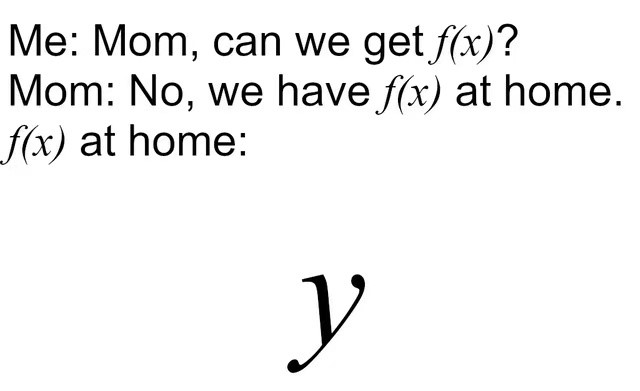
\includegraphics[scale=0.5]{yathome.jpg}
  \end{figure}


\chapter{运算与代数结构\\ Opérations et Structure Algébrique}
  
  \section{运算}
  在我的数学学习经历中,我最先认识了数字,也就是1、2、3、4这些,随后就开始学习了加法,然后是减法、乘法、除法之类的东西.
  这些东西都被称为运算.有些运算是一元的,例如$\cos x$和$|x|$,我们输入一个变量,得到一个返回结果;有些运算是二元(多元)的,例如$a^b$或者$A \times B$.本章里我们主要讨论二元运算.
  有些运算与数没有关系,例如逻辑运算里,$1\vee 0=1$,这里1和0只是表示逻辑上的真和假,与具体的数字无关.
  此外,还有一种题目叫做“定义新运算”,一般会给出一个自定义的算符,比如$\star $,然后解释这个算符怎么计算,比如说$a\star b=114a+\frac{514}{b}-19^{\frac{a}{b}}$,让你求解一些具体的返回值.
  这些统统都是运算.为了应付日益复杂的数学,我们需要把运算统一起来研究,以便于尝试找到普适性的规律.\label{myref:traditionalcalculate}
  \subsection{Définition}
  给定集合$X$,所有$f:X\times X\rightarrow X$的映射称为集合$X$上的运算.直观上看,运算将$X$上的有序点对映射为$X$的元素.
  我们姑且将运算符号记为$\star $.
  这样我们可以将一个运算表示为$(x,y)\in X*2,f(x,y)\rightarrow x\star y$.
  \subsubsection{Exemple}
  在$\R$上两个区间的并$(-114,81]\cup (-91,514)=(-114,514)$是一个运算.
  \subsection{结合律 Associative}
  设$X$上的运算$f(x,y)\rightarrow x\star y $,若:
  $$
  \forall (x,y,z)\in X^3, x\star(y\star z)=(x\star y)\star z
  $$
  称此运算满足结合律.
  \subsection{交换律 Commutative}
  设$X$上的运算$f(x,y)\rightarrow x\star y $,若:
  $$
  \forall (x,y)\in X^2, x\star y=y\star x
  $$
  称此运算满足交换律.
  \subsection{中性元/单位元 l'élément neutre/identité}
  单位元又叫中性元.设$X$上的运算$f(x,y)\rightarrow x\star y $,若:
  $$
  \forall x\in X, \exists e\in X,e\star x=x
  $$
  称$e$是左单位元,若:
  $$
  \forall x\in X, \exists e\in X,x\star e=x
  $$
  称$e$是右单位元,若$e$同时为左单位元及右单位元,则称$e$为单位元.
  单位元也被记作$\Id$,即identité的前两个字母.或者在很多地方都有自己的记号.
  \subsubsection{Exemple}
  $\R $上的加法单位元为0,乘法单位元为1.幂运算$a\star b=a^b$的右单位元为1,没有左单位元.
  \subsubsection{Exemple}
  集合$X$上交集运算的单位元为$X$,并集运算的单位元为$\varnothing $.
  \subsubsection{Exemple}
  设集合$A=\{e,f\}$上的运算为:
  $$
    \begin{aligned}&
    e\star e=f\star e=e\\&
    f\star f=e\star f=f
  \end{aligned}
  $$则$e,f$都是左单位元.
  \subsubsection{Proposition:单位元唯一}
  一个运算如果有单位元,则单位元是唯一的.
  \subsubsection{Démonstration}
  $\lnot (\text{单位元是唯一的})\Rightarrow \exists (e_1,e_2)\text{都是单位元}\Rightarrow e_1\star e_2=e_1,e_1\star e_2=e_2\Rightarrow e_1=e_2$
  \subsubsection{Remarque}
  一个运算有若干个左单位元是可能的.
  事实上,每一个元素都可以是左单位元.同样地,右单位元也一样.
  但若同时存在有右单位元和左单位元,则它们会相同且只存在一个单位元.
  
  \subsection{可逆元/可对称元 Symétrique}
  设$X$上的运算$f(x,y)\rightarrow x\star y $有单位元$e$,若:
  $$
  \forall x\in X, \exists x'\in X,x'\star x=e
  $$
  称$x'$是左可对称的,若:
  $$
  \forall x\in X, \exists x'\in X,x\star x'=e
  $$
  称$e$是右可对称的.所有满足$x\star x'=x'\star x=e$的$x'$称为$x$的可对称元.使用乘法符号时一般把可对称称为可逆,$x'$记作$x^{-1}$.
  
  \section{符合结合律的有单位元运算}
  符合结合律且有单位元的运算具有一些有趣的性质.本节讨论均假设$X$上满足结合律的运算$f(x,y)\rightarrow x\star y $有单位元$e$.
  \subsection{可对称元唯一性}
  当且仅当左对称元$x'$和右对称元$x''$是唯一且相同时,$x$是可对称的.
  \subsubsection{Démonstration}
  $$
    x''=e\star x''=(x'\star x)\star x''=x'\star(x\star x'')=x'\star e=x'
  $$
  \subsection{可对称的运算不变性}
  若$x$和$y$是可对称的,则$x\star y$也可对称,且$(x\star y)'=y'\star x'$.
  \subsubsection{Démonstration}
  $$
    (y'\star x')\star(x\star y)=y'\star (x'\star x)\star y=y'\star e\star y=y'\star y=e
  $$反过来同理.
  \subsection{解的唯一性}
  设$a$可对称,对于$b$,仅有唯一一个$x$使得$a\star x=b$,即$x=a'\star b$.
  \subsubsection{Démonstration}
  $$
    a\star x=b\Rightarrow a'\star b=a'\star (x\star x)=(a'\star x)\star x=e\star x=x
  $$反过来同理.
  这意味着,例如,在乘法中,形如$ax=b$的方程有且仅有唯一解$x=a^{-1}b$.

\section{代数结构 Structure Algébrique}
  在数学中,代数结构由非空集合$A$和$A$上的运算集合(通常是二元运算)和一组有限的恒等式(公理)组成,这些运算必须满足这些公理.
  研究代数结构的好处在于,当一个新问题涉及与这种代数结构相同的定律时,仅使用结构定律证明的所有结果都可以直接应用于新问题.
  \subsubsection{Exemple}
  $\R$上的加法$(\R,+)$就是一个代数结构,其具有以下公理:
  \begin{itemize}
    \item 交换律:$a+b=b+a$.
    \item 结合律:$(a+b)+c=a+(b+c)$.
    \item 单位元0:  $a+0=0+a=a$.
    \item 可逆性:$a+(-a)=(-a)+a=0$.
  \end{itemize}
  \subsubsection{Exemple}
  回看前言里\prettyref{myref:abstract}所展现的分析学知识,可见大部分内容都与代数结构相关.
  \subsection{封闭性}
  当我们想使用一个代数结构,也就是对一个集合上的元素进行运算时,为了得到一些良好的性质或者进行后续的运算,
  我们通常希望运算的结果能拥有一些性质.最简单的就是这个结果可以再次被拿来运算.这意味着这个运算结果也属于代数结构的集合.
  也即$$\forall (x,y)\in A\times A, x\star y=z \Rightarrow z\in A$$这样的性质称为封闭性.


  想象一个没有封闭性的代数结构上的运算,比如$\R$上,某个运算结果为:$1\star 4=\text{西红柿炒鸡蛋}$.
  显然,1和4都在$\R$上,但是西红柿炒鸡蛋不属于$\R$,我们也并不清楚西红柿炒鸡蛋有什么性质,它与$\R$上的元素有什么关系,也不能拿来继续运算.这样的性质就很糟糕.\\
  
  现在,我希望你假装忘记掉曾经学习的这些运算,也就是\prettyref{myref:traditionalcalculate}开头我提到的那些以前的东西(特别是加法和乘法),以便我们从另一个角度重新出发学习它们.

\section{群 Groupe}
  \subsection{Définition}
  群是一种代数结构,依托于集合上的运算"$\times$",称为"乘法",记为$(G,\times)$或者$(G,\cdot)$(有时运算符号可省略).
  为了避免与笛卡尔积混淆,我们统一采用$(G,\cdot)$记号.
  其满足以下公理:
  \begin{itemize}
    \item 封闭性:$\forall(a,b)\in G^2,a\cdot b=c\in G $.
    \item 结合律:$\forall(a,b,c)\in G^3,(a\cdot b)\cdot c=a\cdot (b\cdot c) $.
    \item 单位元e: $\forall a\in G, \exists e\in G, a\cdot e=e\cdot a=a$.
    \item 可逆性:  $\forall a\in G, \exists a^{-1}\in G, a\cdot a^{-1}=a^{-1}\cdot a=e$.
    \item \textbf{Bonus:}交换律:$\forall(a,b)\in G^2,a\cdot b=b\cdot a $.
  \end{itemize}
  满足前四项公理的代数结构称为群.额外满足第五项交换律的群称为"阿贝尔群(Groupe Abélien)".
  \subsubsection{Exemple}
  \begin{itemize}
    \item 整数的通常意义加法$(\mathbb{Z},+) $构成群,但是通常意义乘法$(\mathbb{Z},\cdot) $不构成群,因为不满足有可逆元.
    \item (n阶非奇异矩阵\footnote{万一你还没学过这个定义,它意味着矩阵的行列式值不等于0.},矩阵乘法)是一个群.



  \end{itemize}
  \subsection{阶 Ordre}
  在有限群范围内,群$(G,\cdot)$的阶等于集合$G$里元素的个数,也就是$|G|=\text{card }G$.
  元素的阶等于让该元素通过幂运算得到单位元的最小幂,也就是$n_{min},a^n=e$.

  \subsection{乘法表 Table de multiplication}
  乘法表常被用来表示简单的群上的元素和运算,它列举了群内任意两个元素的乘积.下面我们通过一个简单的例子来理解乘法表.
  \subsubsection{$C_3$群}\label{myref:C_3}
  想象一个等边三角形$\Delta ABC$,我们将它绕着垂直于几何中心的州进行旋转操作:
  \begin{itemize}
    \item 操作a:顺时针旋转120°
    \item 操作b:逆时针旋转120°
    \item 操作e:不旋转
  \end{itemize}
  我们发现,经过操作a后,原来的A点变成了B点,B点变成了C点,C点变成了A点,得到了三角形$\Delta BCA$.
  而与此同时,经过两次操作b后也能让原来的A点变成了B点,B点变成了C点,C点变成了A点.也就是说,两次操作b与一次操作a等价.同理,两次操作a与一次操作b等价.
  进一步地,我们发现,三次操作a、三次操作b、操作b后操作a、操作a后操作b与操作e相互都是等价的.如果我们把操作看作一个集合,操作的复合看作运算$\cdot $,就得到了一个群.其中的运算关系如下:
    \begin{itemize}
    \item $a=b\cdot b=a\cdot e$
    \item $b=a\cdot a=b\cdot e$
    \item $e=e\cdot e=a\cdot a\cdot a=b\cdot b\cdot b=a\cdot b=b\cdot a$
    \end{itemize}
  这个群被称为$C_3$群.其阶数为3,元素a和b的阶数也是3.
  将这些运算关系组合成一个表,第一行表示在运算符号前的元素,第一列表示运算符号后的元素,就可以填入所有的运算结果.也即:
  \begin{table}[!h]
    \centering
    \begin{tabular}{r|lll}
         ($C_3,\cdot$) & \textbf{a} & \textbf{b} & \textbf{e} \\ \hline
        \textbf{a} & b & e & a \\ 
        \textbf{b} & e & a & b \\ 
        \textbf{e} & a & b & e \\ 
    \end{tabular}
    \caption{$C_3$群的乘法表}
    \label{C_3times}
  \end{table}
  \subsection{重排定理 Théorème de réarrangement}
  考虑代数结构$(A,\star)$,对$a\in A$,定义$a\star A=\{ a\star a_\alpha|a_\alpha \in A \}$.对群$G$,有:
  $$
  \forall a\in G,a\cdot G=G\cdot a=G
  $$也即群内的每个元素和某个元素相乘得到的仍然是原来的群,这被称为群的重排定理.
  \subsubsection{Démonstration}
  由运算的封闭性知$a\cdot G\subseteq G$,
  由可逆性知$\forall (a,g)\in G\times G, \exists (a'\cdot g)\in G\text{使得}g=a\cdot (a'\cdot g)=g\Rightarrow g\in a\cdot G\Rightarrow G\subseteq a\cdot G$.
  \subsection{生成元 Générateur}
  生成元是描述一个群的重要方式.下面我们由循环群开始逐渐介绍生成元和其应用方法.
  \subsubsection{循环群 Groupe cyclique}
  由一个元素$R$及其幂次构成的有限群称为由$R$生成的循环群,记为$C_n$,其中\n 为循环群的阶,$R$称为循环群的生成元.
  这就是为什么\prettyref{myref:C_3}介绍的群叫$C_3$群.在$C_3$群中,a和b都是其生成元.对于\n 阶循环群, 其阶数等于其生成元的阶数.
  \subsubsection{有限群的生成元与秩 Générateur et rang d'un groupe fini}
  对任一有限群, 是否同样有生成元呢?答案是肯定的,由此还能引出有限群的秩的概念.对有限群$G$,任取一元素$R_1$,得到其幂次构成的集合$\mathbf{R_1}$.
  若$\mathbf{R_1}^C\neq \varnothing$,即无法填满整个群,则在$\mathbf{R_1}^C$内任取一元素$R_2$并得到$\mathbf{R_2}$,以此类推.
  将选取的元素组成集合$\{R_i\}$,该集合即为群$G$的生成元,且$\text{card}\{R_i\}$称为群的秩.
  \subsubsection{Proposition}
  有限群的生成元的选择不唯一,但秩不变.

  \section{从原群到群 De magma à groupe}
  一个代数结构想成为群需要符合四个条件,那不能全部符合四个条件的代数结构又是什么呢?
  \subsection{原群 Magma}
  对代数结构$(E,\star)$,若其运算满足封闭性,则该代数结构为一个原群.

  \subsection{半群 Demi-groupe}
  对原群$(E,\star)$,若其运算满足结合律,则该原群为一个半群.

  \subsection{幺半群 Monoïde}
  对半群$(E,\star)$,若其含有中性元,则该半群为一个幺半群.

  \subsection{拟群 Quasigroupe}
  对原群$(E,\star)$,若有:
  $$
  \forall (a,b)\in E\times E, \exists (x,y)\in E\times E\text{使得}a\star x=y\star a=b
  $$则该原群为一个拟群.


  \begin{figure}[H]
    \centering
    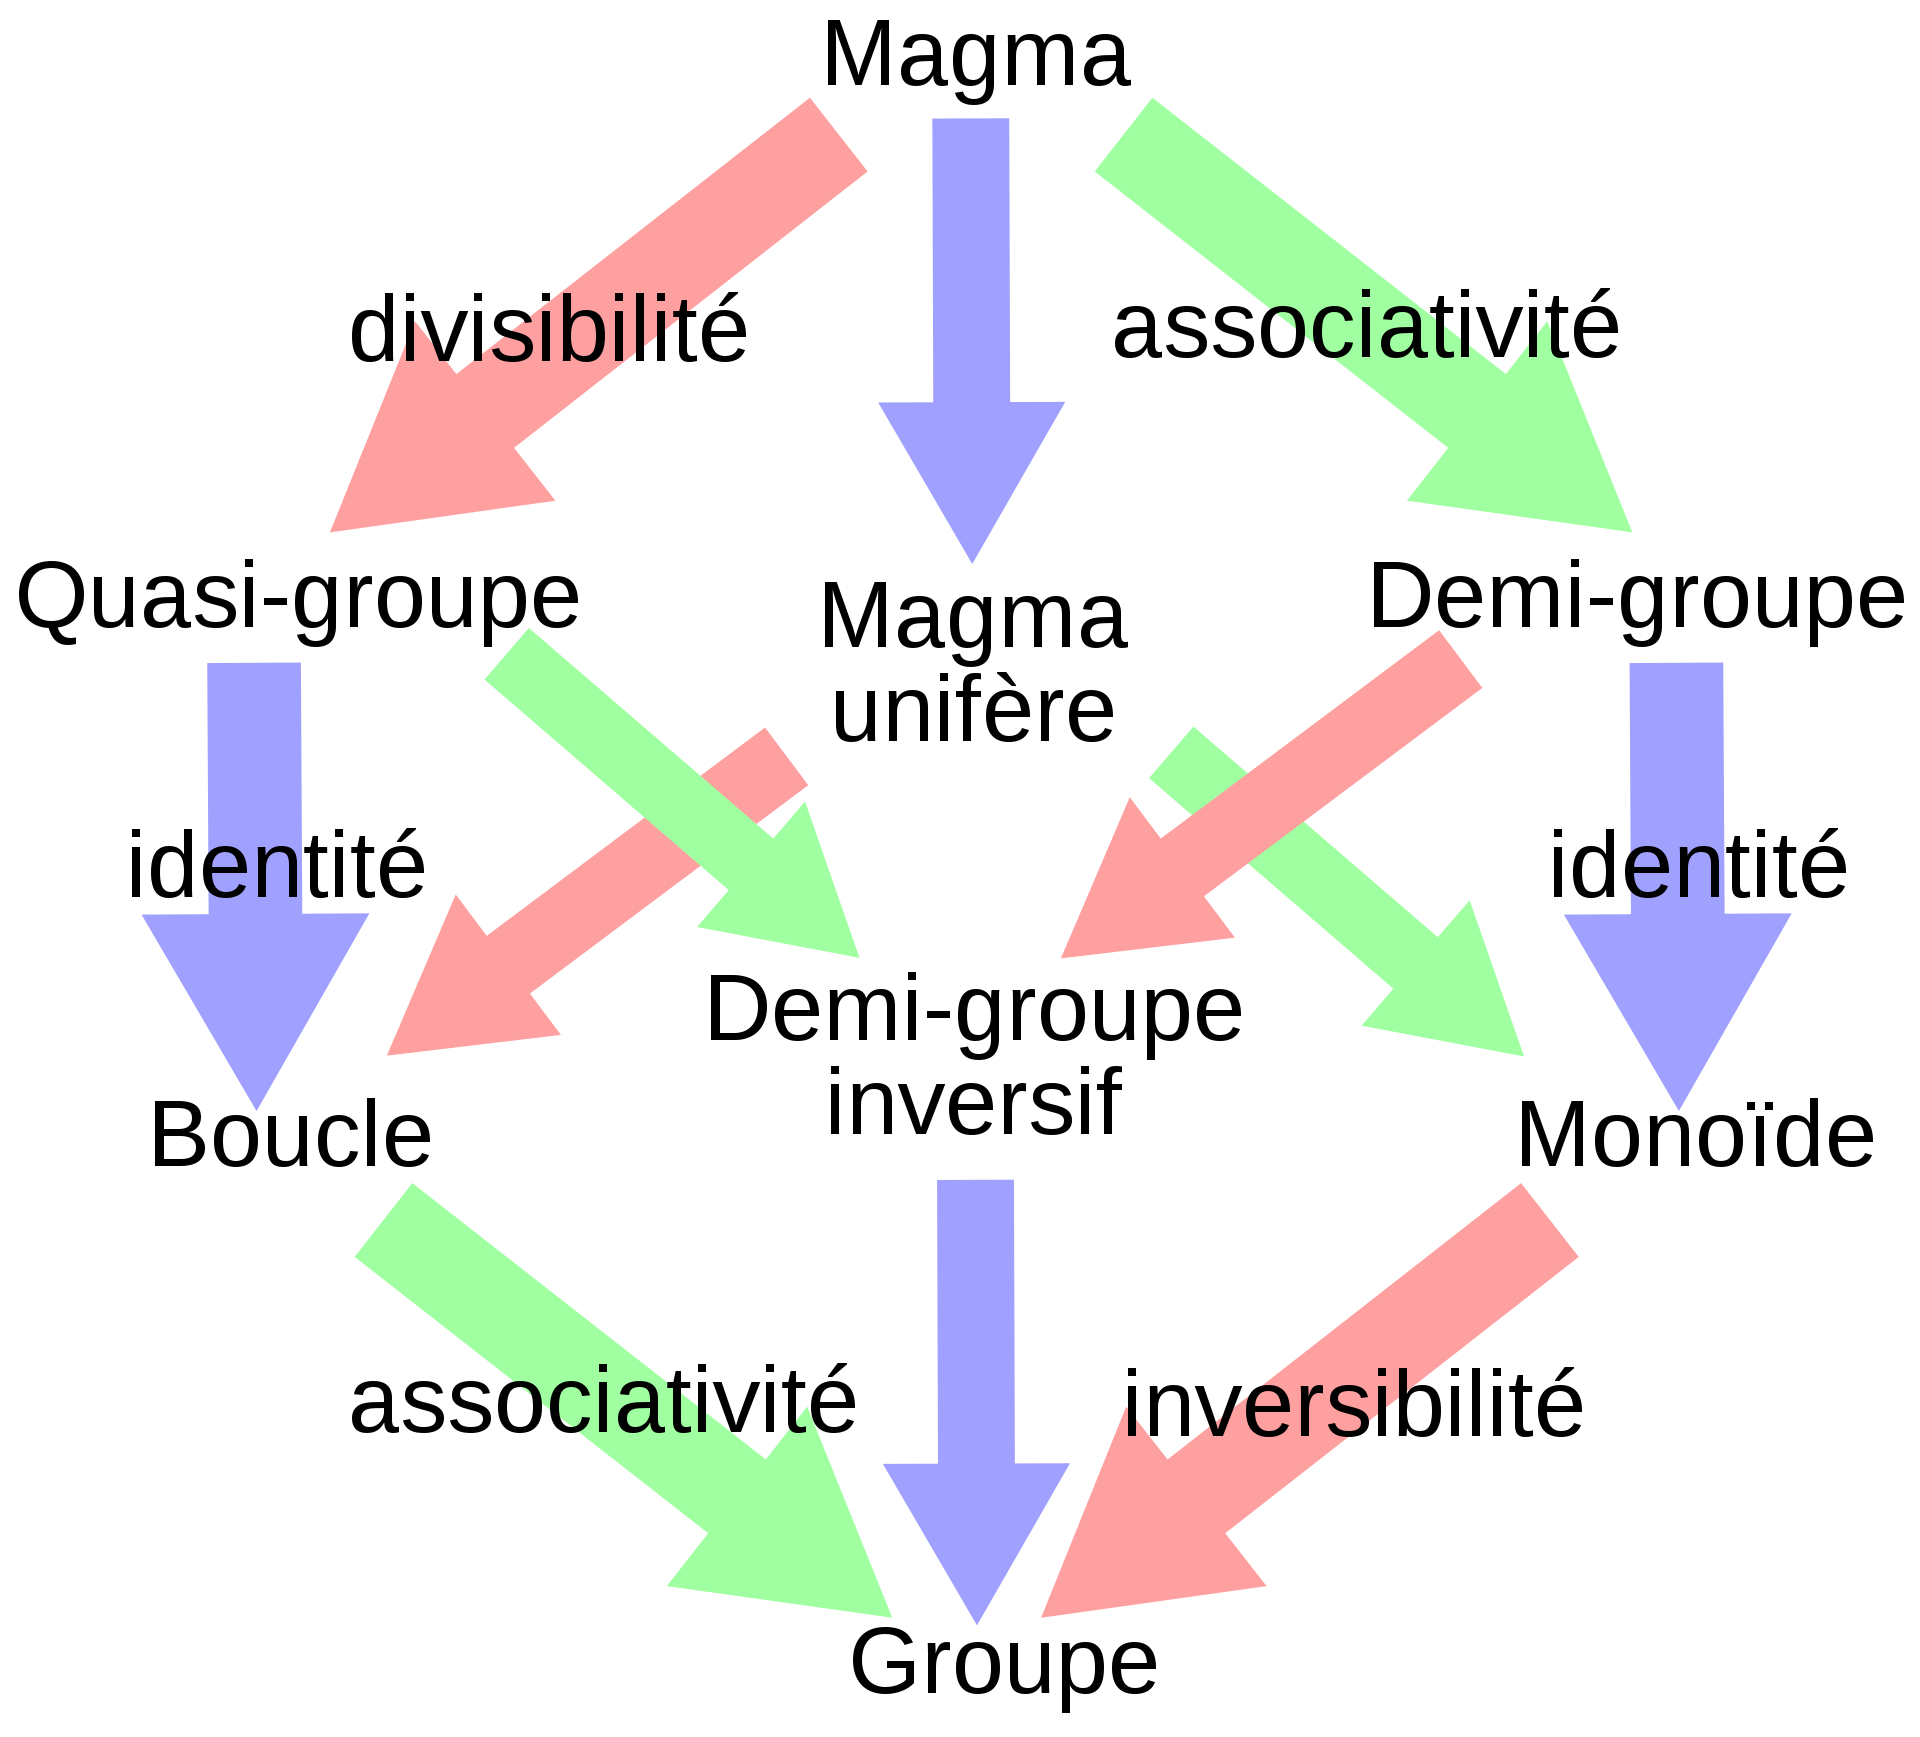
\includegraphics[scale=0.13]{magma_groupe.png}
    \caption{从原群到群(图源wiki)}
    \label{myref:groupe_magma}
  \end{figure}

  \section{群论基础 La Théorie Rudimentaire des Groupes}
  在数学中,特别是在一般代数中,群论是研究群的代数结构的学科.群论的发展起源于数论、代数方程理论和几何学,在理论物理、化学、材料科学和非对称密码学中有多种应用.
  本章只对群论内容做一个基础的、入门的介绍.事实上,关于群、环和域相关的知识在本讲义中并不怎么重要,很多结论也不会有后续应用(所以有相当多平凡的推论我没有写出证明,摸了).但是有些概念和定义还是会用上的,因此我还是简单地列出来.

  \subsection{共轭关系 Conjugaison}\label{myref:conjugaison}
  定义二元关系~为:对$(a,b)\in G\times G, \exists g\in G$使得$b=g^{-1}\cdot a\cdot g$.称该关系为共轭关系,a~b为a与b共轭.
  \subsubsection{Proposition}
  共轭关系是等价关系.
  \subsubsection{Démonstration}
  \begin{itemize}
    \item $a=a^{-1}\cdot a\cdot a\Rightarrow a\sim a$
    \item $a\sim b\Rightarrow b=g^{-1}\cdot a\cdot g\Rightarrow g\cdot b\cdot g^{-1}=a\Rightarrow a=(g^{-1})^{-1}\cdot b\cdot g^{-1}\Rightarrow b\sim a$
    \item $b=g^{-1}\cdot a\cdot g, c=f^{-1}\cdot a\cdot f\Rightarrow b=f\cdot c\cdot f^{-1}=g^{-1}\cdot a\cdot g\Rightarrow c=(f^{-1}\cdot g^{-1})\cdot a\cdot (g\cdot f)\Rightarrow c\sim a$
  \end{itemize}
  \subsubsection{共轭类 Action par conjugaison}
  a的共轭类是群内所有与其共轭的元素组成的集合,记为$Cl(a)$或$C_a$,即$Cl(a)=\{g\cdot a\cdot g^{-1}|g\in G\}$.\\

  接下来给出一些共轭类的简单推论:
  \subsubsection{Proposition}
  $a\sim b\Leftrightarrow Cl(a)\cap Cl(b)\neq \varnothing$
  \subsubsection{Proposition}
  共轭类内元素的阶相同.
  \subsubsection{Proposition}
  单位元e只与自己共轭.
  \subsubsection{Proposition}
  Abel群里每个元素只与自己共轭.
  \subsubsection{Proposition}
  $a\sim b\Rightarrow \forall k\in \mathbb{N},a^k\sim b^k$.

  \subsection{子群 Sous-groupe}
  直观上说,子群就是群的一个同样是群的子集.
  \subsubsection{Définition}
  对群$(G,\cdot)$,若$H\subseteq G$使得$(H,\cdot)$也是一个群,则称$H$是$G$的子群.
  \subsubsection{Proposition}
  $G$和$\{e\}$显然都是子群.它们被称为平凡子群(sous-groupe trivial)或者 sous-groupe impropre.
  不是平凡子群的子群称为特征子群(sous-groupe propre).
  \subsubsection{Remarque}
  质数阶(或者1阶)循环群没有特征子群.
  \subsubsection{Proposition}
  对于$pq$阶循环群($p,q$为正整数),其只有一个$p$阶子群.该子群是由$g^q$生成的循环群.

  \subsection{陪集 Classe suivant un sous-groupe}
  法语里并没有专门的陪集的专有名词,而是直接叫classe suivant un sous-groupe,这是个很形象的说法.英语称陪集为coset,其实也和suivant有异曲同工之妙吧.
  \subsubsection{Définition}
  群$(G,\cdot)$有子群$H$.对任意$g\in G$,$H$有如下两个陪集:
  \begin{itemize}
    \item 左陪集(classe à gauche de $g$ suivant $H$): $gH=\{g\cdot h|h\in H\}$
    \item 右陪集(classe à gauche de $g$ suivant $H$): $Hg=\{h\cdot g|h\in H\}$
  \end{itemize}
  \subsubsection{陪集分解 Décomposition en classes suivant un sous-groupe}
  群$G$可以被分解成若干个左陪集的并,或者若干个右陪集的并.对应的分解称为左/右陪集分解.即:
  $$
  G=\bigcup_{\alpha\in G}\alpha H= \bigcup_{\alpha\in G}H\alpha
  $$
  \subsubsection{Proposition}
  $f\in gH\Leftrightarrow fH=gH,f\in Hg\Leftrightarrow Hf=Hg$.
  \subsubsection{Proposition}
  $gH=H\Leftrightarrow g\in H\Leftrightarrow Hg=H$.
  \subsubsection{Proposition}
  $|gH|=|H|$
  \subsubsection{Proposition}
  “属于同一左陪集”是一个等价关系.
  \subsubsection{Proposition}
  任意两个左陪集要么不相交要么相等.

  \subsection{群论的Lagrange定理 Théorème de Lagrange}
  Lagrange定理的直接叙述为:子群的阶整除群的阶,即:若群$(G,\cdot)$有子群$H$,则$|G|=k|H|,k\in\mathbb{N}$.
  将其倍数$k$记为$[G:H]$,表示$H$在$G$中左陪集的个数.
  \subsubsection{Démonstration}
  考虑子群$H$关于$G$内所有元素的左陪集组成的集族$\mathbb{H}=\{g_iH|g_i\in G\},\text{每个左陪集的阶都相同,}|g_jH|=|g_kH|$并且$\sum_{i}^{\text{card }\mathbb{H}}|g_iH|=|G|$
  此时$\text{card }\mathbb{H} $就是$[G:H]$.
  \subsubsection{Proposition}
  素数阶的群只有平凡子群,没有特征子群.
  \subsubsection{Proposition}
  元素的阶整除群的阶.(元素的阶可以组成子群)
  \subsubsection{Fermat小定理 Théorème de Fermat}
  对整数$a$和素数$p$,若$a$不是$p$的倍数,则$a^p-1$是$p$的倍数,即:
  $$
    a^{p-1}\equiv 1(\mod p)
  $$
  \subsubsection{Démonstration}
  为了证明这个推论,我们考虑$G=\{1,2,\dots , p-1\}$和模运算组成的群.假设$a\equiv b(\mod p),\text{显然}b\in G$.
  设$b$的阶数为$k$,即$b^k\equiv 1(\mod p)$,则可得到子群$H=\{a,b,\dots ,b^{k-1}\}$则$k$可以整除$G$的阶数,也就是$p-1$.
  此时再设$p-1=km$,此时有:
  $$
    a^{p-1}\equiv b^{km}\equiv (b^k)^m\equiv 1^m\equiv 1(\mod p)
  $$得证.
  \subsection{正规子群 Sous-groupe normal}
  正规子(Sous-groupe normal) 又叫不变子群(Sous-groupe invariant),法语里还有称Sous-groupe distingué.其代表共轭变换下不变的子群.
  \subsubsection{Définition}
  对群$(G,\cdot)$,若子群$N$满足:
  $$
  \forall n\in N,\forall g\in G,g\cdot n\cdot g^{-1}\in N
  $$则称$N$是$G$的正规子群,记作$N\lhd G$或者$N\unlhd G$.
  \subsubsection{等价条件}
  下列条件等价于子群N在G中是正规子群:
  \begin{itemize}
    \item $\forall g\in G,gNg^{-1}\subseteq N $
    \item $\forall g\in G,gN=Ng $
    \item $\forall (g,h)\in G\times G,gh\in N\Leftrightarrow hg\in N$
  \end{itemize}


  \subsection{商群 Groupe quotient}
  \subsubsection{子群的乘法}
  设群$(G,\cdot)\text{有子群}H\text{和}F$,定义其乘法为:
  $$
  H\cdot F=\{h\cdot f|(h,f)\in G\times F \}
  $$
  \subsubsection{Définition}
  利用正规子群的左陪集和右陪集相同的这个特点将群按照陪集的方法进行分割.
  分割后的所有陪集形成的集合能够形成一个新的群,称之为商群,记为$G/H$.也即:
  $$
  G/H=\{gH\text{ }|H\lhd G,g\in G \}
  $$
  \subsubsection{Démonstration}
  \begin{itemize}
    \item 单位元: $aH=H=Ha$
    \item 逆元: $aH\cdot a^{-1}H=aa^{-1}HH=H$
    \item 结合律: $aH\cdot bH\cdot cH=(ab)cH=a(bc)H=aH\cdot(bH\cdot cH) $
    \item 封闭性: $aH\cdot bH=(ab)H\in G/H $
  \end{itemize}
  \subsubsection{Proposition}
  $|G/H|=[G:H]$,商群的阶是群的阶除以子群的阶的商.
  \subsubsection{Proposition}
  若$(G,\cdot)$是Abel群/循环群/有限生成群,则$G/H$也是.

  \subsection{同态 Homomorphisme}    \label{myref:Homomorphisme}
  \subsubsection{Définition}
  同态是两个群之间的一种特殊的映射,其概念非常直观.“同”表示映射的两端有什么东西是一样的,或者不变的.“态”就是群的某种“状态”.
  群只有集合和运算两个要素,集合映射过去后不可能保持不变,那能保持的也就只有运算了.因此,同态就是两个群之间保持乘法运算的映射,即
  对于$(G,\cdot)$和$(H,\star)$上的映射$f:G\rightarrow H $,若
  $$
    \forall (x,y)\in G\times G,f(x\cdot y)=f(x)\star f(y)
  $$称$f$是$(G,\cdot)$和$(H,\star)$上的同态映射.存在同态映射的两个群是同态的.若同态是单射,则称单同态(Monomorphisme),若为满射则称满同态(Épimorphisme).
  \subsubsection{Exemple}
  正实数上通常加法群到通常乘法群上的映射$f(x)=e^x$就是一个同态.$e^{a+b}=e^a\cdot e^b$.
  \subsubsection{Proposition}
  同态的一个重要性质是保证了单位元映射到单位元,$f(e_G)=e_H$.
  \subsubsection{自同态 Endomorphisme}
  群$(G,\cdot)$到自身上的同态映射称为自同态.
  \subsubsection{态射 Morphisme}
  同态的推广被称为态射.在讨论群的内容时,法语有时直接用态射指代同态,记住两者在此时是同一概念.
  \subsection{同构 Isomorphisme}    \label{myref:Isomorphisme}
  若同态映射$f$为双射,则称为同构映射,两个群是同构的,记作$G\cong H$.
  \subsubsection{Proposition}
  同构是等价关系.

  \subsubsection{自同构 Automorphisme}
  同理,群$(G,\cdot)$到自身上的同构映射称为自同构.
  \subsubsection{Remarque: 同构与相等}
  一般来说,如果忽略掉同构的对象的属性或操作的具体定义,单从结构上讲,同构的对象是完全等价的.
  但这并不意味着同构就是相等.例如,我们很容易知道$C_3$群可以和某个群\{西红柿炒鸡蛋,醋溜土豆丝,糖醋排骨\}同构(例如
  $f(a)=\text{西红柿炒鸡蛋},f(b)=\text{醋溜土豆丝},f(e)=\text{糖醋排骨}$),
  但这并不代表两个群,或者两个集合就是相等的.起码西红柿炒鸡蛋不在$C_3$群里面.

  \subsection{核 Noyau}
  \subsubsection{Définition}
  对于同态$f:G\rightarrow H $, $G$中映射到$H$单位元的元素称为同态的核,记作:
  $$
  \ker f=\{f(g)=e_H\text{ }|\text{ }g\in G  \}
  $$
  \subsubsection{Proposition}
  $\ker f\lhd G$,核是正规子群.
  \subsubsection{Proposition}
  $G/\ker f\cong H$,核的商群与$H$同构.\\
  
  其实到这里我想接着讲同构基本定理的,
  但是这一章内容太多了,而且毕竟不是写代数讲义,因此我们点到为止,快速过完这一章的内容.


  \section{环 Anneau}
  \subsection{Définition}
  与群类似,环也是一种代数结构,依托于集合上的运算“$+$”和“$\times$”,分别被称为“加法”和“乘法”.同样将乘法符号记为$\cdot$,
  则一个环写作$(R,+,\cdot)$.其满足以下公理:\\

  \noindent
  1.$(R,+)$是Abel群,即:
  \begin{itemize}
    \item 封闭性:$\forall(a,b)\in R^2,a+b=c\in R $.
    \item 结合律:$\forall(a,b,c)\in R^3,(a+ b)+ c=a+ (b+ c) $.
    \item 单位元0: $\forall a\in R, \exists 0\in R, a+0=0+a=a$.
    \item 可逆性: $\forall a\in R, \exists -a\in R, a+(-a)=(-a)+a=0$.有时将此类运算用减法符号代替,即$a+(-b)=a-b$,这样就熟悉多了.
    \item 交换律:$\forall(a,b)\in R^2,a+b=b+a$.
  \end{itemize}
  

  \noindent
  2.$(R,\cdot)$是幺半群,即:
  \begin{itemize}
    \item 封闭性:$\forall(a,b)\in R^2,a\cdot b=c\in R $.
    \item 结合律:$\forall(a,b,c)\in R^3,(a\cdot b)\cdot c=a\cdot (b\cdot c) $.
    \item 单位元1: $\forall a\in R, \exists 1\in R, a\cdot 1=1\cdot a=a$.
  \end{itemize}


  \noindent
  3.乘法对于加法满足分配律,即:
  \begin{itemize}
    \item 左分配:$\forall(a,b,c)\in R^3,a\cdot (b+ c)=(a\cdot b)+(a\cdot c)$.
    \item 右分配:$\forall(a,b,c)\in R^3,(b+ c)\cdot a=(b\cdot a)+(c\cdot a)$.
  \end{itemize}


  \indent
  值得注意的是,在1960年代以前,多数抽象代数的书籍并不将乘法单位元列入环的必要条件中;
  而1960年代后的书籍则更倾向将乘法单位元列入环的必要条件中.
  那些不要求乘法单位元为环的必要条件的作者可能会把包含乘法单位元的环给称为“单位环(Anneau Unitaire/Unifère)”,
  与之相对地,那些要求乘法单位元为环的必要条件的作者,可能会把不包含乘法单位元的环给称为“伪环(Pseudo-anneau,Rng)”.
  \subsubsection{Exemple}
  实数上的通常加法和乘法可以构成很多环,如$(\R,+,\times),(\mathbb{Z},+,\times),(\mathbb{Q},+,\times)$都是环,并且乘法也是可交换的.与群一样,如果乘法满足交换律则称为$Abel$环.
  \subsubsection{Exemple: 多项式环}
  所有形如$P(X)=\sum_{i=0}^{n}a_iX_i $的多项式可以构成一个环.这要求$a_i$必须是某个环$R$上的元素,而$X$视作一个变量的形式符号.
  \subsubsection{Exemple: 矩阵环}
  所有$n\times n$阶的矩阵可以和矩阵加法/矩阵乘法构成一个环.例如$\mathcal{M}_n(\R)$.
  \subsection{环的性质}

  \subsection{特殊的环}
  \subsubsection{整环 Anneau Intègre}
  设$(R,+,\cdot)$是一个交换环且加法和乘法的单位元不相同$(1\neq 0)$.若满足:
  $$
  \forall (a,b)\in A^2,a\cdot b=o\Rightarrow a=0\text{或}b=0
  $$则称该环是一个整环.
  \subsubsection{唯一分解环 Anneau Factoriel,UFD}
  对一个整环$(R,+,\cdot)$,如果其中的每个元素都可以表示为一个可逆元和若干个不可约元素的乘积,即:
  $$
  \forall x\in R,\exists (u,p_1,\dots,p_n)\in R^{n+1},n\in \mathbb{N},x=u\cdot p_1\cdot...\cdot p_n
  $$
  并且
  $$
  x=u\cdot p_1\cdot...\cdot p_n=v\cdot q_1\cdot...\cdot q_m\Rightarrow n=m
  $$
  则称该环是一个唯一分解环.
  \subsubsection{主理想 Idéal Principal}
  若某环$(R,+,\cdot)$的子集$I$为在原环加法的定义下的子群$(I,+)$,且其中的元素在原环乘法下与任意原环中的元素结果都在该子群中,则称其为原环的理想(Idéal).即满足:
  \begin{itemize}
    \item 左理想: $\forall (i,r)\in I\times R,i\cdot r\in I$
    \item 右理想: $\forall (i,r)\in I\times R,r\cdot i\in I$
  \end{itemize}
  每个理想均可由单个元素生成的环称为主理想环.\\


  \section{域 Corps}
  \subsection{Définition}
  域是一种特殊的环,和一般的环的区别在于域要求它的非零元素可以进行除法运算,这等于说每个非零的元素都要有乘法逆元.域中的运算关于乘法是可交换的.
  在域上我们有了熟悉的四则运算的表示(是的,我们终于学到了小学数学的内容,多么伟大!):
  \begin{itemize}
    \item $  a+(-b)=a-b $
    \item $ a\cdot b^{-1}=a/b$
  \end{itemize}
  \subsubsection{Exemple}
  域可以说是我们最熟悉的代数结构了.实数域$(\R,+,\cdot)$,复数域$(\mathbb{C},+,\cdot)$,有理数域$(\mathbb{Q},+,\cdot)$是最常见的域.
  \subsubsection{Exemple}
  一个域的元素如果是有限个,则被称为有限域.例如最小的有限域Boole值域只含有元素$0,1$.
  其满足加法$0+0=0,1+0=1,1+1=0$和乘法$0\cdot 0=0,0\cdot 1=0,1\cdot 1=1$.
  \subsection{域的性质}
  \subsubsection{非零元素的集合}
  域$\mathbb{K}$上所有非零元素构成的集合$\mathbb{K}^x$是一个关于乘法的Abel群,其每个有限子群都是循环群.
  \subsubsection{特征 Caractéristique}    \label{myref:tezheng}
  若存在$n\in \mathbb{N}$使得$n\cdot 1=0$,则称最小的\n 为域的特征.$n=0$表示特征不存在.
  \subsubsection{有序域 Corps Ordonné}
  若可以在域$\mathbb{K}$上定义序关系,则称该域是一个有序域.例如有理数域和实数域上具有通常的序关系.
  \subsubsection{交换环的理想}
  一个交换环是域当且仅当它的理想只有自身和零理想.


  关于群、环和域的更多内容将在代数课程中详细展开.

\chapter{从自然数到有理数\\ Des nombres naturels aux nombres rationnels}
\section{自然数集的公理化 Axiomatique de l'ensemble des nombres naturels}
  \subsection{Peano公理 Axiome de Peano}
  关于自然数,每个人都知道,就是$\N=\{1,2,3,\dots\}$.但这显然不是一个好的定义,因为这样的定义并不清楚自然数的性质.
  比如说,3后面是什么数?114在哪里?它和前后的数有什么关系?于是,我们需要对自然数进行公理化.
  这部分工作主要是在十九世纪后半叶由意大利数学家Giuseppe Peano在德国数学家Richard Dedekind的工作上完善得到的,因此被称为Peano公理:


  设集合$X$和集合上的映射$\S$,若满足:
  \begin{enumerate}
    \item $x\in X$
    \item $x\notin \S(X)$
    \item $\S$是一个单射
    \item \footnote{即数学归纳公理}对于$A\subseteq X$,若$x\in A$且$\forall a\in A,\,\S(a)\in A$,则$A=X$
  \end{enumerate}
  则称$X$是自然数集$\N$,其元素称为自然数.$x$称为初始元素,$\S$称为后继映射,$\S(x)$称为$x$的后继元素.
  此时可以认为:
  $$
  \N=\{x,\S(x),\S^2(x),\dots,\S^n(x),\dots\}
  $$
  在通常意义下,认为$x=0$,即:
  $$
  \N=\{0,1,2,\dots,n,\dots\}
  $$
  对于不含0的自然数集,则称为正整数集$\N^*$.
  \subsection{自然数集中的加法运算 Addition dans l'ensemble des nombres naturels}
  根据自然数集的特点, 可以分两步“归纳地” 定义自然数的加法. 
  首先定义任一自然数和初始元的加法规则,然后假定已经知道了任一自然数与$n$的加法规则, 在此假定下规定任一自然数与$n$的后继元的加法规则. 由数学归纳原理可知, 这样就定义了任意两个自然数的加法规则.
  也就是:
  \begin{flalign*}
    \N\times \N & \longrightarrow  \N\\
    (n,m) & \longmapsto  n+m\\
  \end{flalign*}
  该映射满足:
  $$
  \begin{cases}
    n+1=\S(n)\\
    n+\S(m)=\S(n+m)
  \end{cases}
  $$
  则称该映射为加法.显然有$\S^n(a)=a+n$.
  \subsubsection{关于加法的一些结论}
  以下是一些简单的关于加法的结论.其证明过程都非常简单,基本上就是利用归纳法先证明某个数为0的情况,然后一步步加上去即可.故为了节省篇幅,我直接给出结论.
  \begin{enumerate}
    \item 交换律:$\forall (a,b)\in \N^2,a+b=b+a$
    \item 结合律:$\forall (a,b,c)\in \N^3,(a+b)+c=a+(b+c)$
    \item 消除律:$\forall (a,b,c)\in \N^3,a+b=a+c\Leftrightarrow b=c$
    \item $\forall b\in \N^*,\,\exists a\in \N,\,\S(a)=b$
    \item $\forall a\in\N^*,\,\forall b\in\N,\,a+b\in\N^*$
    \item $a,b\in\N\text{且}a+b=0 \Leftrightarrow a=b=0$
  \end{enumerate}
  \section{自然数集上的序关系 Relations d'ordre sur l'ensemble des nombres naturels}



  \section{整数集的构造 Construction de l'ensemble des nombres entiers}
  \section{整数集中的运算 Opérations dans l'ensemble des nombres entiers}
  \section{整数集上的序关系 Relations d'ordre sur l'ensemble des nombres entiers}
  \section{有理数集的构造 Construction de l'ensemble des nombres rationnels}
  \section{数域 Corps}
  \section{有理数域上的序关系 Relations d'ordre sur l'ensemble des nombres rationnels}



\chapter{实数\\ Nombres Reéls}%扩展多个章节
  \section{实数域的构造 Construction de l'ensemble des nombres réels}
  \section{Dedekind分割 Coupure de Dedekind}
  \section{实数集上的序关系 Relations d'ordre sur l'ensemble des nombres réels}
  \section{实数域的完备性 Complétude de l'ensemble des nombres réels}


\chapter{可数性\\ Dénoembrabilité}
  本章将研究两种不同类型的无限集:可数集和不可数集,并阐明什么是可数,什么不可数.
\section{基数 La cardinalité}
  \subsection{Définition}
  定义关系$\sim$.基数指集合中元素的个数,又叫势
  \footnote{在某些语境下,势的概念只用于比较两个无穷集的元素多寡,而不能直接指称某集合的元素个数.在一般语境下,尤其是当一切都定义好了以后,也经常使用势作为基数的同义词}.
  对于集合A和B,若当且仅当存在双射$f:A\rightarrow B$时,称$A\sim B$,即A和B拥有相同的基数.
  \subsection{有限集 Finite}
  设集合$A$,若$A=\varnothing$或者$\exists n\in\N^*,\,A\sim \{1,2,\dots,n\}$,则称$A$是有限集.
  \subsubsection{Proposition}\label{myref:youxianji}
  对有限集$A$和$B$,$\text{card}A=\text{card}B\Leftrightarrow A\sim B$.
  \subsubsection{Démonstration}
  \noindent $\Rightarrow$:\\
  设$A=\{a_1,a_2,\dots,a_n\},B=\{b_1,b_2,\dots,b_n\}$有双射$f:a_i\rightarrow b_i\Rightarrow A\sim B$\\

  \noindent $\Leftarrow$:\\
  1.$\forall x\in A, \exists y\in B,\text{使得} f(x)=y\Rightarrow\text{card}A\leq\text{card}B$\\
  2.$\forall y\in B, \exists x\in A,\text{使得} f^{-1}(y)=x\Rightarrow\text{card}B\leq\text{card}A$\\
  $\Rightarrow \text{card}A=\text{card}B$
  \subsection{Proposition}\label{myref:carddengjia}
  势是等价关系.
  \subsubsection{Démonstration}
  \noindent
  1.$A\sim A:\forall x\in A, f:x\rightarrow x$即为所求双射.\\
  2.$A\sim B\Rightarrow B\sim A: f^{-1}$即为所求双射.\\
  3,$A\sim B,B\sim C\Rightarrow A\sim C:f:x\rightarrow y,g:y\rightarrow z,f\circ g $即为所求双射.\\
  
\section{可数性 Dénoembrabilité}
  可数性的定义非常贴近生活.想一想,平时你怎么计数?比如数一数本讲义共有几章呢?1,2,3,4,...
  计数的记号显然属于自然数集合$\mathbb{N}$.于是很自然地,我们认为一个集合如果能用自然数这样一个一个数出来,就说明它是可数的.
  \subsection{Définition}
  \noindent 
  \begin{itemize}
    \item 对集合$A$,若$A\sim\mathbb{N} $称它是可数的(dénoembrable).
    \item 若集合$A$有限或可数,称$A$是至多可数的(au plus dénoembrable).
    \item 若集合$A$无限且不可数,称$A$是不可数的(indénombrable).
\end{itemize}
  \subsubsection{可数集的基数}
  可数集的基数定义为$\aleph_0$.
  \subsection{Exemple}\label{myref:Zkeshu}
  $\mathbb{Z}$是可数的.我们可以找到双射$f:\mathbb{N}\rightarrow\mathbb{Z}$:
  $$
    f(n)=\begin{cases}
    \frac{n}{2} &n=2k\\
    \frac{1-n}{2} &n=2k+1
    \end{cases}
  $$
  \subsection{Proposition}
  若$A\sim B$则$A,B$同属于"有限""无限可数""不可数"三种类型之一.
  \subsubsection{Démonstration}
  \noindent
  1.有限:见 \prettyref{myref:youxianji}\\
  2.无限可数:$A\sim \mathbb{N}$,由等价关系(\prettyref{myref:carddengjia})可知$\mathbb{N}\sim A\Rightarrow\mathbb{N}\sim B$则$B$无限可数.\\
  3.无限不可数:$\lnot(B\text{可数})\Rightarrow\mathbb{N}\sim B\Rightarrow\mathbb{N}\sim A\Rightarrow\bot$故$B$不可数.\\
  需注意:逆命题对3不成立.两个不可数集不一定能一一对应.

\section{无限集的可数性 Dénoembrabilité des ensembles infinis}
  \subsection{Définition}
  无限集是指至少与他的一个真子集的势相同的集合.对集合$A$,若:
  $$
    \exists B\subset A, B\sim A
  $$
  称$A$是一个无限集.
  \subsection{Exemple}
  设$S$是区间$(0,1)$上所有元素的集合,则$S$是不可数集.\\

  那么,如何证明$S$是不可数集?如果$S$是不可数集,那么当我们选取$S$的一个可数子集$E$时,$S$中应该还有一些不包含在 E 中的元素,对吧?
  也就是
  $$
    \forall E\subset S,E\sim \mathbb{N}\Rightarrow \exists x\in S,x\notin E 
  $$
  因此,如果我们可以证明$S$的每个可数子集都是一个真子集,那么$S$就是不可数集.
  这是因为如果$S$的每个可数子集都是一个真子集并且$S$是可数集,那么$S$本身就是它自己的一个真子集,这是不可能的!
  这基本上意味着无论我们如何计数$S$中的元素,总会有一些元素被漏掉.
  \subsubsection{Démonstration}
  这里我们用到了著名的Cantor对角线法.我们把每个$S$中的元素都用一个无限小数表示出来
  \footnote{我们不加证明地认为每个实数都可以写成一个无限小数},形如$0.d_1d_2d_3d_4\dots$.
  现在尝试选出可数集$E$,排列成:
  $$
  \begin{aligned}&
    e_1=0.d_{1,1}d_{1,2}d_{1,3}d_{1,4}\dots\\ &
    e_2=0.d_{2,1}d_{2,2}d_{2,3}d_{2,4}\dots\\ &
    e_3=0.d_{3,1}d_{3,2}d_{3,3}d_{3,4}\dots\\ &
    e_4=0.d_{4,1}d_{4,2}d_{4,3}d_{4,4}\dots\\ &
    e_5=0.d_{5,1}d_{5,2}d_{5,3}d_{5,4}\dots\\ &
    \vdots 
      \end{aligned}
  $$
  那么这个任意的$E$包含了$S$中的所有元素吗?错!我们可以找到这样一个数
  $$s=s_1s_2s_3s_4\dots\text{使得}s_i\neq d_{i,i}$$
  这意味着$s$与第1个数的第1位小数不一样,与第2个数的第2位小数不一样,与第3个数的第3位小数不一样$\dots$
  也就是与$E$中每个数都不一样,显然不属于$E$.
  这里构造$s$的方法沿着上面那个有点像矩阵一样的东西的对角线一直走下去,所以叫对角线.
  该方法由集合论的创始人康托尔(Cantor)提出,故称为Cantor对角线法.
  \subsection{可数集的笛卡尔积 Countable Union of Countable Sets}
  设$n$个可数集$C_1,C_2,\dots,C_n$,则其笛卡尔积$C_1\times C_2\times\dots\times C_n$是可数的.
  \subsection{可数子集}
  任意无限集$S$都有可数子集.

  \subsubsection{Démonstration}
  先取一个$a_1$,取完后剩下的集合不是空集,故可以以此类推一直取下去.
  \subsection{最小基数 Cardinalité minimale}
  无限集的最小基数是$\aleph_0$.
  \subsubsection{Démonstration}
  利用反证法,设无限集$A$有$\card A<\aleph_0$,则存在一个可数子集$A_1\sim\N$.即:
  $$
  \aleph_0=\card A_1\leq\card A<\aleph_0
  $$
  故矛盾.
  
  \subsection{子集可数关系 }
  \noindent
  设$E\subseteq A$,则有:\\
  $A\text{至多可数}\Rightarrow E\text{至多可数}$\\
  $E\text{不可数}\Rightarrow A\text{不可数}$
  \subsection{Proposition:可数集可数并可数}\label{myref:keshujikeshubingkeshu}%可数集可数并可数%
  考虑可数个集合$E_i$:
  $$
  E_i\sim\mathbb{N},S=\bigcup_{i=1}^\infty E_i\Rightarrow S\sim\mathbb{N}
  $$
  \subsubsection{Démonstration}
  有点复杂,哪天想起来再慢慢画.
  \subsubsection{Remarque}
  对于可数集的不可数并,这个结果是错误的.
  \subsubsection{Proposition}
  可数集任意可数并可数.
  \subsubsection{Proposition}
  $\R$不可数.
  \subsection{Proposition:可数集元组可数}\label{myref:Rnkeshu}
  设$A$是可数集,$A^n$是由$A$中元素构成的全体\n 元组的集合,那么$A^n$是可数的.
  \subsubsection{Démonstration}
  数学归纳法,先证明$A^1$可数,再假设$A^{i+1}$可数,得出$A^n$是可数集的可数并,于是$A^n$至多可数.
  详细证明留给读者.
  \subsection{Proposition:有理数集可数}
  一个简化的证明过程:我们知道任何有理数都可以写成$\frac{p}{q},(p,q)\in\mathbb{Z}^2$的形式,
  并且\prettyref{myref:Zkeshu}告诉我们$\mathbb{Z}$是可数的,\prettyref{myref:Rnkeshu}告诉我们$\mathbb{Z}^2$是可数的.
  显然$\mathbb{Z}^2$的一个子集可以与$\mathbb{Q}$构造双射,所以$\mathbb{Q}$是可数的.

  \subsection{Proposition:无理数集不可数}
  一个简单的证明过程:我们知道$\R=\mathbb{Q}\cup\mathbb{I}$,且$\mathbb{Q}$是可数的.
  若$\mathbb{I}$是至多可数的,则根据\prettyref{myref:keshujikeshubingkeshu}可知$\R$是至多可数的,这显然矛盾.
  故$\mathbb{I}$是不可数的.
  
  \subsection{Cantor-Bernstein定理 Théorème de Cantor-Bernstein}
  设$A,B$是两个集合,$A_1\subset A,\,B_1\subset B$,
  若存在双射$f:A\rightarrow B_1,g:B\rightarrow A_1$,则$A\sim B$.
  %结束了,2023新年快乐!
  \section{代数数和超越数 Nombres algébriques et nombres transcendants}
  \subsection{Définition}
  对实数$x$,若其满足多项式方程:
  $$
  \sum_{i=0}^{n}a_ix^{n-i}=0
  $$
  其中$a_0\in\Z^*,\,a_1,\dots,a_n\in\Z$,则称$x$是一个代数数(nombre algébrique).否则,称$x$是一个超越数(nombre transcendant).
  \subsection{Proposition}
  由代数数全体组成的集合是可数的.
  \subsubsection{Démonstration}

  本节内容待补充.
  \section{连续统 Continuum}
  \subsection{Définition}
  对集合$A$,若$A\sim\R$,则称$A$是连续统.
  连续统的基数称为连续基数或连续统势(cardinal du continuum),记作$\aleph_1$或$\mathfrak{c}$.
  \subsection{Exemple}
  \begin{itemize}
    \item $\R$上的任一区间是连续统.
    \item 全体超越数组成的集合是连续统.
    \item 平面上的点集是连续统.
  \end{itemize}
  \subsection{Cantor定理 Théorème de Cantor}
  设非空集合$A$,则$A$的幂集$\mathcal{P}(A)$的基数大于$A$的基数,也即:
  $$
  \card A<\card \mathcal{P}(A)
  $$
  \subsubsection{Démonstration}
  $A$是有限集时显然成立.设$A=\{a_I\}$是无限集,假设$\card A=\card \mathcal{P}(A)$,则存在双射$f:A\rightarrow \mathcal{P}(A)$.
  设$B=\{a_I\in A\,|\,a_I\notin f(a_I)\}$.显然$B\in\mathcal{P}(A)$,但不存在$f(a_\lambda)=B$,故$f$不是满射,矛盾.
  \subsubsection{Proposition}
  Cantor定理表明,不存在最大的基数.因为对于任意集合$A$,总有基数更大的集合$\mathcal{P}(A)$.
  \subsection{可数集幂集的势}
  可数集幂集的势等于连续基数.
  $$
  \card \mathcal{P}(\N)=2^{\aleph_0}=\aleph_1
  $$
  \subsubsection{Démonstration}
  设集合$A=\{0,1\},\,J=A^\infty$.考虑映射:
  \begin{flalign*}
    f:\mathcal{P}(\N)&\rightarrow J\\
    E&\rightarrow (a_1,a_2,\dots)
  \end{flalign*}
  其中
  $$a_i=\begin{cases}
    1 &i\in E\\
    0 &i\notin E
  \end{cases}$$
  $f$是单射.由映射的关系知道$\forall \alpha=(a_1,a_2,\dots),\,\exists!E\in \mathcal{P}(\N),\,f(E)=\alpha$.
  故\f 是双射.有
  $$
  \card \mathcal{P}(\N)=\card J=2^{\aleph_0}=\aleph_1
  $$
  \subsection{连续统假设 Hypothèse du continu}
  1874年Cantor提出了连续统假设,即不存在基数介于$\aleph_0$和$\mathfrak{c}$之间的集合.
  1940年Kurt Friedrich Gödel证明了连续统假设和集合的ZFC公理系统不矛盾,即ZFC 理系统无法证伪连续统假设.
  1963年Cohen进一步证明连续统假设无法被ZFC公理系统证明.



\chapter{复数与Euclide空间\\Nombre Complexe et Espace Euclidien}%扩展多个章节

\chapter{初等数论\\ Théorie Élémentaire des Nombres}
  \section{素数和最大公因子 Nombres premiers et Plus Grand Commun Diviseur}
  \section{同余 Congruence}
  \section{乘性函数 Fonction Multiplicative}
  \section{原根 Racine Primitive}
  \section{二次剩余 Quadratic Residue}
  \section{Gauss整数 Gauss Entier}


\part{数学分析里的空间\\ Espaces dans l'Analyse}

\chapter{数列与数项级数\\Suites et Séries}

\chapter{$\R$上的一元函数\\ Fonctions d'Une Variable Réelle}

\chapter{Riemann积分\\ Intégrale de Riemann}

\chapter{函数列与函数项级数\\Suites et Séries de Fonctions}
  本章所研究的两个概念都是由以前学习过的数列(suite)和级数(série)推广而来.
  其中,函数列是数列的推广,函数项级数是数项级数的推广,二者都是以数列和级数的理论为基础建立.
  研究函数列和函数项级数,是为了用一种全新的方法定义函数,并讨论函数的性质,特别是收敛性(convergence)和连续性(continuité).
  基于此,我们可以研究算子的换序问题.

\section{函数列与函数项级数}
  \subsection{Définition}
  函数列指各项为具有相同定义域的函数的序列.
  I是$\R$上的区间,$\mathcal{F}(I)$是区间I上所有函数的集合.
  对一个有序列${f_n}\in\mathcal{F}(I)$,称${f_n}$为一个函数列.
  后续会一直默认${f_n}\in\mathcal{F}(I)$这个条件.\\

  函数项级数可以被简单地理解为函数列的加和.
  对于一个函数列${f_n}$,其函数项级数为$S_p=\sum_{n=0}^{p} f_n$,其中$p\in\mathbb{N}$.\\
  \subsection{Remarque:二者的关系}
  函数项级数和函数列有着密切的关系,正如数列和数项级数那样,
  一个函数项级数可以认为是某个函数列的构成的数列的前\n 项和,
  而函数列${f_n}$可以认为是函数项级数$S_p=\sum_{n=1}^{p} f_n-f_{n-1}$, $p\in\mathbb{N}, f_0=0$的\n 次部分和.
  因此函数列以及函数项级数的性质可以等价,我们只需要研究其中一个,自然就可以得到两个的结论.


\section{逐点收敛 Convergence simple}
  逐点收敛是函数列最基本的收敛,可以直观地理解为函数列${f_n}$里每个函数$f_i$定义域中,每个点$x$组成的数列${x}_n$随n都是收敛的.
  \subsection{Définition}
  逐点收敛的一种定义为:
  \begin{equation}
    \notag
    \forall x\in I, f_n(x)\xrightarrow[n\rightarrow\infty]{}f(x)
  \end{equation}
  此时称函数列$f_n(x)$在区间$I$上逐点收敛于$f(x)$ (La suite $f_n(x)$ convergence simplement vers $f(x)$ sur $I$).\\
  同理,对于函数项级数:
  \begin{equation}
    \notag
    \forall x\in I, \sum_{n=0}^{p} u_n(x)\xrightarrow[n\rightarrow\infty]{}U(x)
  \end{equation}
  称函数项级数$u_n(x)$在区间$I$上逐点收敛于$U(x)$.
  
  
  \subsection{Proposition:逐点收敛的算子交换}
  本章所研究的主要是针对于极限算子、Riemann积分算子和求导算子的交换问题.
  显然,对于逐点收敛这么弱的结论,三种算子都是不可交换的.\\
  \subsubsection{极限算子}
  设$I=[0,1] , f_n(x)=x^n$.显然$f_n$在区间$I$上有逐点收敛
  \begin{equation}
    \notag
    f_n\xrightarrow[n\rightarrow\infty]{}f=
    \begin{cases}
    0 &x\in[0,1)\\
    1 &x=1
    \end{cases}
  \end{equation}
  \begin{equation}
    \notag
    \lim_{n \to \infty} \lim_{x \to 1} x^n=1 \mbox{,然而由于$f$在1处不连续,} 
    \lim_{x \to 1}\lim_{n \to \infty} x^n \mbox{不存在}
  \end{equation}
  故极限算子无法交换.
  \subsubsection{求导算子}
  同上,$f$在1处不连续,故不可导,故求导算子无法交换.
  \subsubsection{Riemann积分算子}
  设$I=[0,1] , s_n(x)=2n^2xe^{-n^2x^2}$.显然$f_n$在区间$I$上逐点收敛于$s(x)=0$
  \begin{equation}
    \notag
    \lim_{n \to \infty} \int_{0}^{1}  2n^2xe^{-n^2x^2}=1 \mbox{,然而}
    \int_{0}^{1}\lim_{n \to \infty} 2n^2xe^{-n^2x^2}=0 
  \end{equation}
  故Riemann积分算子无法交换.


\section{一致收敛 Convergence uniforme}
  \subsection{界 La borne}
  \subsubsection{Définition}
  设函数$f(x)$在集合$D$上有定义.若存在$K$使得对任意$x\in D, f(x)\leq K$,则称$f(x)$在集合$D$上是有上界的(majoré).
  对于最小的上界$k$,称其为函数$f(x)$在集合$D$上的上确界(le supremum),记为$k=\sup f(x)$.
  \subsubsection{Remarque:有界}
  特别地,若存在正数$M$使得对任意$x\in D, |f(x)|\leq M$,则称$f(x)$在集合$D$上是有界的(borné).

  \subsection{Définition}
  一致收敛的一种定义为:
  \begin{equation}
    \notag
    \|f_n-f \|_\infty
    \footnote{此记号为$L^\infty$范数,后续说明.}
    =\sup_{x\in I}| f_n(x)-f(x)|\xrightarrow[n\rightarrow\infty]{}0   
  \end{equation}
  此时称函数列$f_n$在区间$I$上一致收敛于$f$ (La suite $f_n$ convergence uniformément vers $f$ sur $I$).\\
  同理,对于函数项级数:
  \begin{equation}
    \notag
    \|\sum_{n=0}^{p} u_n-U \|_\infty=\sup_{x\in I}| \sum_{n=0}^{p} u_n(x)-U(x)|\xrightarrow[p\rightarrow\infty]{}0  
  \end{equation}
  称函数项级数$u_n(x)$在区间$I$上一致收敛于$U(x)$.\\

  一致收敛相比于逐点收敛是个强结论.逐点收敛中不同点对应的“收敛速度”可能不同,但一致收敛中各点收敛的速度具有一致性.
  如果$f_n$在区间$I$上一致收敛于$f$,则$f_n$一定在区间$I$上逐点收敛于$f$.
  \subsection{Proposition:连续性的传递}
  若函数列$f_n$在区间$I$上一致收敛于$f$,且$\forall n\in\mathbb{N}, f_n\in\C ^0(I)$,
  则$f\in\C ^0(I)$
  \subsection{Proposition:等价条件}
  \noindent
  以下五个命题等价:\\
  1.$f_n(x)$一致收敛于$f(x)$\\
  2.$\forall \epsilon>0 \exists N\in \mathbb{N}^*, x_0\in I. n>N\Rightarrow | f_n(x)-f(x) |<\epsilon$ \\
  3.$d(f_n,f)\xrightarrow[n\rightarrow\infty]{}0$\\
  4.$\sup_{x\in I}| f_n-f|\xrightarrow[n\rightarrow\infty]{}0$\\
  5.$\forall \{x_n\}\subseteq I,f_n(x_n)-f(x_n)\xrightarrow[n\rightarrow\infty]{}0 $\\
  其中,5常用于否定一致收敛.
  \subsection{判断一致收敛}
  \subsubsection{方法1.}
  找到一个独立的、只与n有关的上界函数,证明该函数趋近于0.即:
  \begin{equation}
    \notag
    \sup_{x\in I}| f_n(x)-f(x)|\leq g(n)\xrightarrow[n\rightarrow\infty]{}0   
  \end{equation}
  \subsubsection{方法2.}
  若$f_n$和$f$都在$I$上可导,则求出他们差的极大值趋近于0,即:
  \begin{equation}
    \notag
    g(x)_{\max}=|f_n(x)-f(x)|_{\max}\xrightarrow[n\rightarrow\infty]{}0   
  \end{equation}
  \subsection{Proposition: 一致收敛的算子交换}
  与逐点收敛这种弱结论不同,一致收敛有许多优秀的性质,可以帮助我们交换算子.
  \subsubsection{极限算子1.}
  若函数列$f_n$在区间$I$上一致收敛于$f$,且$\forall n\in\mathbb{N}, \exists l_n\in\R$使得
  $\lim_{x \to x_0}f_n(x)=l_n$,则有:
  \begin{equation}
    \notag
    \lim_{n \to \infty}l_n= \lim_{n \to \infty}\lim_{x \to x_0}f_n(x)
    =\lim_{x \to x_0}\lim_{n \to \infty}f_n(x)=\lim_{x \to x_0}f(x)   
  \end{equation}
  \subsubsection{极限算子2.}
  若函数列$f_n$在区间$I=[a,\infty), a\in\R$
    \footnote{$I=(-\infty,a], a\in\R$时将$x \to \infty$换成$x \to -\infty$仍然成立.}
  上一致收敛于$f$,且$\forall n\in\mathbb{N}, \exists l_n\in\R$使得
  $\lim_{x \to x_0}f_n(x)=l_n$,则有:
  \begin{equation}
    \notag
    \lim_{n \to \infty}l_n= \lim_{n \to \infty}\lim_{x \to \infty}f_n(x)
    =\lim_{x \to \infty}\lim_{n \to \infty}f_n(x)=\lim_{x \to \infty}f(x)   
  \end{equation}
  \subsubsection{Riemann 积分算子}
  若函数列$f_n$在区间$I=[a,b], (a,b)\in\R^2$
  上一致收敛于$f$,且$\forall n\in\mathbb{N}, f_n\in\C ^0([a,b])$,则有:
  \begin{equation}
    \notag
    \lim_{n \to \infty}\int_{a}^{b} f_n(x)
    =\int_{a}^{b} \lim_{n \to \infty}f_n(x)=\int_{a}^{b} f(x)   
  \end{equation}
  \subsubsection{求导算子}
  若函数列$f_n$在区间$I=[a,b], (a,b)\in\R^2$上逐点收敛于$f$,
  $f'_n$在区间$I=[a,b]$上一致收敛于$f$,
  且$\forall n\in\mathbb{N}, f_n\in\mathcal{C} ^1([a,b])$,则有:
  \begin{equation}
    \notag
    f'=\frac{\mathrm{d} }{\mathrm{d} x}f
    =\frac{\mathrm{d} }{\mathrm{d} x} \lim_{n \to \infty} f_n
    =\lim_{n \to \infty}f'_n  
  \end{equation}



\section{依范数收敛 Convergence normale}
  依范数收敛\footnote{原课程范数还没讲就把这东西拿出来了,感觉好怪.}%待调整顺序
  的概念是由卡尔·维尔斯特拉斯(Karl Weierstrass)提出,于勒内·拜尔(René Baire)在1907-1908年出版的Leçons sur les théories générales de l'analyse中引入的.
  \footnote{可参考\href{https://fr.wikipedia.org/wiki/Convergence_normale}{wiki:convergence normale}}\\
  \subsection{Définition}
  依范数收敛的一种定义为:
  \begin{equation}
    \notag
    \sum_{n=0}^{\infty}\|f_n(x) \| _\infty=\sum_{n=0}^{\infty}\sup| {f_n(x)}| <\infty
  \end{equation}
  称函数项级数$f_n$在$I$上依范数收敛.注意:我们不关心此时收敛于某个对象.
  \subsection{Remarque:一致收敛与依范数收敛}
  依范数收敛是一致收敛的强结论(自然也是逐点收敛的强结论).依范数收敛的列一定一致收敛,反则不一定.这里举一个例子:
  \begin{equation}
    \notag
    f_n(x)=\begin{cases}
      \frac{1}{n} &x=n\\
      0 &x\neq n
      \end{cases}\\
    \end{equation}
  \begin{equation}
    \notag
    \sum_{n=0}^{\infty}f_n(x)\mbox{一致收敛,然而}
    \sum_{n=0}^{\infty}\sup| {f_n(x)}|=\sum_{n=0}^{\infty}\frac{1}{n}\mbox{发散.}
    \end{equation}
  \subsection{Proposition}


\chapter{一致收敛判别法}
  本节不打算展开讲,只谈判别法本身.详细内容留待以后有空再补充.会附更多例子.
\section{Cauchy判别法}
  $f_n$在$I$上一致收敛,当且仅当:
  \begin{equation}
    \notag
    \forall \epsilon>0, \exists N\in \mathbb{N}, \forall m,n>N,\forall x\in I, | f_n(x)-f_m(x) |<\epsilon
  \end{equation}
  其函数项级数的表示为,$\sum_{i=0}^{p}f_i(x)$在$I$上一致收敛,当且仅当:
  \begin{equation}
    \notag
    \forall \epsilon>0, \exists N\in \mathbb{N}, \forall n>m>N,\forall x\in I, S_n-S_m=|sum_{i=m+1}^{n}f_i(x)|<\epsilon
  \end{equation}
  \subsubsection{Proposition:收敛于0}
  \begin{equation}
    \notag
    \sum_{n=0}^{p}f_n\\
    \mbox{{} 在$I$上一致收敛,则有}\\
    \sup_{x\in I}| f_n(x)|\xrightarrow[n\rightarrow\infty]{}0
  \end{equation}
  \subsubsection{Proposition:绝对收敛}
  \begin{equation}
    \notag
    \sum_{n=0}^{p}| f_n| \\
    \mbox{{} 在$I$上一致收敛,则有}\\
    \sum_{n=0}^{p}f_n\\
    \mbox{{} 在$I$上一致收敛}
  \end{equation}

\section{Weierstrass判别法}
  设正向级数$\sum_{n=0}^{p}a_n$收敛,
  若$\forall(x,n)\in I\times \mathbb{N},|f_n(x)|\leq a_n $则$f_n$在$I$上一致收敛.

\section{Abel-Dirichlet判别法}
  \subsection{Dirichlet判别法}
  若函数列$a_n(x)$对$\forall x \in I$都关于n单调,且在$I$上一致收敛于0;
  函数项级数$\sum_{n=0}^{p}b_n(x)$在$I$上一致有界,则函数项级数$\sum_{n=0}^{p}a_n(x)b_n(x)$在$I$上一致收敛.
  \subsection{Abel判别法}
  若函数列$a_n(x)$对$\forall x \in I$都关于n单调,且在$I$上一致有界;
  函数项级数$\sum_{n=0}^{p}b_n(x)$在$I$上一致收敛,则函数项级数$\sum_{n=0}^{p}a_n(x)b_n(x)$在$I$上一致收敛.\\
  
  Abel判别法与Dirichlet判别法常常一起用,称为A-D判别法.
  

\chapter{度量空间\\Espace métrique}
\section{度量空间}
  度量就是距离的推广,当成距离看就行.
  其概念由莫里斯·勒内·弗雷歇(René Maurice Fréchet)于1906年在著作Sur quelques points du calcul fonctionnel中首次引入.
  \subsection{Définition}
  对集合X,设函数$d:X\times X\rightarrow \R$若$\forall(p,q,r)\in X^3$满足:\\
  1.非负性:$p\neq q,d(p,q)>0,d(p,p)>0$\\
  2.对称性:$d(p,q)=d(q,p)$\\
  3.三角不等式:$d(p,q)\leq d(p,r)+d(r,q)$\\
  称d是一个度量(métrique),$(X,d)$是一个度量空间.
  度量空间中最符合人们对于现实直观理解的为三维欧几里得空间.事实上,“度量”的概念即是欧几里得距离四个周知的性质之推广.欧几里得度量定义了两点间之距离为连接这两点的直线段之长度.
  此外,亦存在其他的度量空间,如椭圆几何与双曲几何,而在球体上以角度量测之距离亦为一度量.狭义相对论使用双曲几何的双曲面模型,作为速度之度量空间.
  度量空间还能导出开集与闭集之类的拓扑性质,这导致了对更抽象的拓扑空间的研究.
                 
  \subsection{Exemple: $\R$上的绝对值}
  最常见、最熟悉的度量,两点之间的距离就是绝对值度量.具有由绝对值给出的距离函数
  $$
  d(x,y) = \vert y - x \vert
  $$
  的实数集合是一个度量空间.

  \subsection{Exemple:离散度量}     \label{myref:lisanduliang}
  定义度量
  $$
  d(x,y)=
  \begin{cases}
    1 & x\neq y\\
    0 & x=y\\
  \end{cases}
  $$
  称度量$d$是离散的(Discrète).这是个简单但重要的例子,可适用于任何非空集合.
  并且,其证明了对于任何非空集合,总是有一个度量空间与之关联.使用此一度量,每个点都是开球,且因此每个子集都是开的,且该空间具有离散拓扑.
  
  \subsection{Exemple: Levenshtein度量}
  又称Levenshtein距离,是编辑距离的一种.指两个字串之间,由一个转成另一个所需的最少编辑操作次数.该距离可被视为一个图中最短路径度量的特例.
  其允许的编辑操作包括:\\
  1.将一个字符替换成另一个字符\\
  2.插入一个字符\\
  3.删除一个字符\\
  例如,字符串"Augustin"和"Bugusetin"的Levenshtein度量为2,即:\\
  
  "Augustin"$\rightarrow$"Bugustin"$\rightarrow$"Bugusetin"


\section{度量空间中的点与集合}
  \subsection{有界集与无界集}
  度量空间$(X,d)$中,对$E\subset X$,若:
  $$
    \exists q\in X , \exists M\in \R\text{使得}\forall p\in E,d(p,q)\leq M
  $$称$E$是有界集;若:
  $$
    \forall q\in X , \forall M\in \R\text{使得}\exists p\in E,d(p,q)> M
  $$称$E$是无界集.
  \subsection{Proposition:有界集有限并有界}
  $$
  \forall n\in \mathbb{N},A_{i,i\in [\![1,n]\!]}\subset X\text{有界}\Rightarrow \bigcup_{i=1}^n A_i\text{有界}
  $$
  \subsubsection{Démonstration}
  利用并集的有限性,考虑$q$与最远的$p_i$的距离,就能找到一个$M_i\ge d(p,q)$.详细证明留给读者.
  \subsubsection{Remarque}
  对于有界集无限并,该命题不成立.

  \subsection{邻域 Le voisinage}     \label{myref:voisinage}
  这是一个很简单但是很重要的概念,它表示一个点"附近"的空间.
  度量空间$(X,d)$中点$p$的邻域$N_r(p)=\{q\in X | d(p,q)<r\}$.例如$\R^2$中任何一个圆的内部都是围绕圆心的邻域.
  \subsection{极限点}
  度量空间$(X,d)$中的集合E,若:
  $$
  \forall r>0, N_r(p)\cap E\neq\{p\}\mbox{且}\neq\varnothing 
  $$
  称p是E的一个极限点.
  \subsubsection{Exemple}
  $(-114,514)$中的每个点都是其极限点,并且"紧贴着"的点$-114$和点$514$也是其极限点,尽管它们甚至都不在这个集合里面.
  然而,一旦不是"紧贴着",就不是极限点了,比如$-114.0019$和点$514.0081$都不是$(-114,514)$的极限点.
  \subsubsection{Proposition}
  若p是E的一个极限点,则邻域$N_r(p)$包含了E中无穷多个点(否则就能找到最小的r了).
  \subsubsection{Proposition}
  若E是有限集,则它没有极限点.
  \subsection{闭集}
  度量空间$(X,d)$中的集合$E$若包含了其所有的极限点,则称$E$是闭集.例如$[-114,514]$就是一个闭集.
  此外,所有的有限集都是闭集,因为它们没有极限点,自然也就包含了"所有的"极限点(哪怕是0个!).
  \subsection{内点}
  对$E\subset X$内的一点$p$,若:
  $$
    \exists r>0\mbox{,使得}N_r(p)\subset E
  $$称点$p$是$E$的内点.内点始终被"包裹"在集合内,没有"外露".

  \subsection{稠密集 La densité}
  定义稠密集为对$E\subset X$:
  $$
  \forall x\in X, x\in E\text{,或者}x{是}E{的极限点}
  $$
  称$E$在$X$上是稠密的(dense).
  \subsubsection{Proposition}
  闭集$E$在$X$上稠密当且仅当$E=X$.
  \subsubsection{Proposition}
  有理数集在$\R$上稠密.

  \subsection{完备集}
  对$E\subset X$,若$E$是闭集且所有点都是其极限点,则称$E$是完备集.
  \subsubsection{Exemple}
  $[-114,514]$是完备集,$[-114,514]\cup\{1919\}$不是完备集,因为1919不是极限点.
  \subsubsection{Proposition}
  空集是完备集.

\section{开集与闭集的性质}
  \subsection{开集}
  对$E\subset X$,若:
  $$
    \forall p\in E, \exists r>0\text{,使得}N_r(p)\subset E
  $$称$E$是$X$上的开集.
  \subsubsection{Exemple}
  $(-114,514)$是开集, $[-114,514)$不是.

  \subsection{Proposition:邻域是开集}
  任何邻域都是度量空间的开集.
  \subsubsection{Démonstration}
  $$
  \begin{aligned}&
  E=N_r(p)\subset X\Rightarrow \exists r>0, \forall q\in E,d(p,q)<r\\ &
  \Rightarrow \exists k>0,d(p,q)<r-k\\ &
  \Rightarrow \forall s\in N_k(q).d(q,s)<k\\ &
  \text{由三角不等式得:}d(p,s)\leq d(p,q)+d(q,s)<r\\ &
  \Rightarrow s\in E\Rightarrow N_k(q)\in E\\ &
  \Rightarrow \forall q\in E, \exists k>0 , N_k(q)\subset E\\ &
  \Rightarrow E\text{是开集}
  \end{aligned}
  $$
  \begin{figure}[H]%插入题目的图片
    \centering
    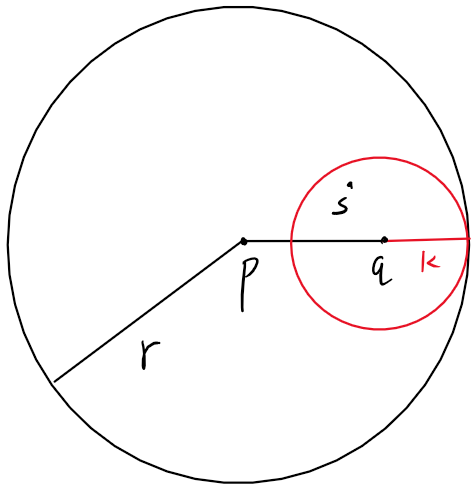
\includegraphics[scale=0.5]{linyushikaiji.png}
  \end{figure}

  \subsection{开集的补集}
  %相对开集与相对闭集
  $\forall E\subseteq X:$
  $$
  E^C\text{是闭集}\leftrightarrow E\text{是开集}
  $$
  \subsubsection{Démonstration}
  \subsubsection{Proposition}
  同理,补集是开集的集合是闭集.
  \subsection{Proposition: 开集的无限并与并集的无限交}
  $$
  \forall \alpha ,U_\alpha\text{是开集}\Rightarrow\bigcup_\alpha U_\alpha\text{是开集}
  $$
  $$
  \forall \beta ,E_\beta\text{是闭集}\Rightarrow\bigcap_\beta U_\beta\text{是闭集}
  $$
  \subsection{Proposition: 开集的有限交与并集的有限并}
  $$
  \forall \alpha ,U_\alpha\text{是开集}\Rightarrow\bigcup_\alpha U_\alpha\text{是开集}
  $$
  $$
  \forall \beta ,E_\beta\text{是闭集}\Rightarrow\bigcap_\beta U_\beta\text{是闭集}
  $$

  \subsection{闭包 L'adhérence}
  内点和极限点组成的几何叫做集合的闭包,记为$\overline{E}$即:
  $$
  \overline{E}=E\cup E'
  $$
  我们会给出一些关于闭包的简单的推论,它们都非常直观.
  \subsubsection{Exemple}
  $(114,514)$的闭包为$[114,514]$.
  \subsubsection{Remarque}
  闭包是闭集.
  \subsection{Proposition}
  与闭包相等的集合是闭集.
  $$
  E=\overline{E}\Leftrightarrow E\text{是闭集}
  $$
  \subsection{Proposition}
  集合$E$的闭包是包含它的最小闭集.
  \subsection{Proposition}
  对度量空间中的子集$E$,若:
  \begin{itemize}
    \item $E$有上界$\Rightarrow \sup E\in \overline{E}$
    \item $E$有下界$\Rightarrow \inf E\in \overline{E}$
  \end{itemize}
  \subsubsection{Démonstration}
  \noindent
  设$y=\sup E$.
  显然,若$y\in E$ 则$y\in \overline{E}$.\\
  若$y\notin E$ 则$\forall\epsilon>0\,\exists x\in E\, y-\epsilon<x<y $,也即$x\in N_\epsilon(y)\cap E$,则$y$是$E$极限点,故$y\in \overline{E}$.\
  $\inf$的证明一样.
  \subsubsection{Remarque}
  上述命题的逆命题不对.例如$[-114,0)\cup(0,514]$ 的上下界都属于该集合,但它不是闭集.
\section{相对开集/相对闭集}
  \subsubsection{Exemple}
  集合的开与闭受到其所在的度量空间的影响.设$E=(-3,3)$,则其在$\R$上是个开集,但是在$\R^2$上不是.
  这说明集合的开性质受到其所在度量空间的影响.为了消除这样的影响,我们需要讨论相对的开集和闭集.
  \subsection{相对开集}
  对度量空间$X$种的集合$E$和一点$q\in X$,若:
  $$
  \forall p\in E\,\exists r>0\,d(p,q)<r \Rightarrow q\in E
  $$
  则称$E$是$X$的相对开集.
  \subsection{Proposition}
  $Y\subseteq X\,,E\subseteq Y\,,G\in X$若$G$是开集,则:
  $$
  E=G\cap Y\Leftrightarrow E\text{是}Y\text{的相对开集}
  $$
  这个概念非常像\prettyref{myref:soustopo}提到的子空间拓扑.
  一个大空间里某个集合的性质仍属于这个集合和一个小空间交出来的集合.
  \subsection{相对闭集}
  对度量空间$X$种的集合$E$和一点$p\in X$,若:
  $$
  \forall p\in X\, \exists r>0\, N_r(p)\cap E\neq \varnothing\land N_r(p)\cap E\neq\{p\}\Rightarrow p\in E
  $$
  则称$E$是$X$的相对闭集.
  \section{紧集}%改到后面
    这部分内容放在这会显得很奇怪,因为在后面拓扑空间里我又会再讲一遍.
    但是为了Heine-Borel定理我又不得不讲清楚.
  \subsection{开覆盖}
  \subsubsection{有限子覆盖}
  \subsection{紧集}
  \subsection{相对紧致}
  \subsection{紧集的性质}
\section{Heine-Borel定理}
  \noindent
  OK,我们简单点,一上来我就把这个定理告诉你:\\
  对$E\subseteq \R^k\, k\in \mathbb{N}$,有:
  $$
  E\text{是紧集}\Leftrightarrow E\text{是闭集}\land E\text{是有界集}
  $$
  很显然,很直观,很一眼得出的结论.但是我们现在想要证明它可不简单.本节剩余的内容都是对这个重要定理的证明.
  \subsection{闭区间套性质}
  设$\R$中的一族闭区间$\{I_n \}\,, \forall n\in \mathbb{N}\,,I_n\subseteq I_{n+1}$,则有:
  $$
    \bigcap_{i=1}^\infty I_i\neq \varnothing
  $$
  闭区间套性质来源于$\R$的最小上界性.事实上这也是一种刻画实数集的方式,每个实数都是这样一族闭区间交集的极限.
  \subsubsection{Démonstration}
  证明非常简单,我已经给出了提示,就是最小上界性.设$I_i=[a_i,b_i]$,考虑闭区间下界组成的集合$E=\{a_i|i\in \mathbb{N}\}$,
  显然这个集合有上界(否则会得到$I_j=[a_j,b_j]\,b_j<a_j$),因此设最小上界$x=\sup E$.此外,$\forall i\in \mathbb{N}\,,b_i$也是$E$的上界,
  故有$x<b_i$,因此有$x\in[a_i.b_i]$.
  \subsection{$k$维格子}
  闭区间套性质不止是用于$\R$,而是可以类似地推广到$\R^k$.
  向量集
  $$\{\textbf{x}=(x_1,\dots,x_k)|x_j\in[a_j,b_j]_{j\in[\![1,k]\!]} \} $$
  称为$k$维格子.
  \subsubsection{Exemple}
  \begin{itemize}
    \item 1维格子就是上文提到的闭区间.
    \item 2维格子是一个封闭的矩形.
    \item 3维格子是一个长方体.
  \end{itemize}
  \subsection{$k$维格子的嵌套性质}
  设$\R^k$中的一族闭$k$维格子$\{I_n \}\,, \forall n\in \mathbb{N}\,,I_n\subseteq I_{n+1}$,则有:
  $$
    \bigcap_{i=1}^\infty I_i\neq \varnothing
  $$
  \subsubsection{Démonstration}
  这里的证明是闭区间套性质证明他推广,请读者自行尝试.只需要证明存在一组$x*=(x_1*,\dots,x_n*)$属于所有的$I_n$就行.

  \subsection{$k$维格子的紧致性}
  $k$维格子是紧集.
  \subsubsection{Démonstration}

  \subsection{Proposition}
  设$\R^k$中的子集$E$,则有:
  $$
  E\text{有界}\Leftrightarrow\exists I=\{\textbf{x}=(x_1,\dots,x_k)|x_j\in[a_j,b_j]_{j\in[\![1,k]\!]} \}\in \R^k\,, E\subseteq I
  $$
  \subsection{Heine-Borel定理}
  对$E\subseteq \R^k\, k\in \mathbb{N}$,有:
  $$
  E\text{是紧集}\Leftrightarrow E\text{是闭集}\land E\text{是有界集}
  $$
  \subsubsection{Démonstration}
  \noindent
  $\Rightarrow$:\\
  $\Leftarrow$:\\

  \subsection{实紧集的极限点}
  $\mathbb{R^k}$的子集$E$是紧集$\Leftrightarrow$$E$的每个无限子集在其中都有一个极限点.
  \subsubsection{Démonstration}
  \subsection{Weierstrass定理}

  \section{完备集与连通集}
  \subsection{Cantor三分集}
  \subsection{分离集}
  \section{压缩映射 Applications contractante}\label{myref:yasuoyingshe}

  

\chapter{赋范空间\\Espace Vectoriel Normé}
  这一章的核心概念是范数(模)的推广.把以前所学习的范数抽象化,然后推广应用.
\section{范数 La norme}
  范数是映射,也是泛函.对于以前学习过的模长,我们发现其具有非负性、绝对齐次性和三角不等式三个优秀的性质,于是我们将其提取出来并推广,重新定义范数.
  \subsection{Définition}
  给定映射:
  $$
  \Vert \cdot \Vert : \mathbb{E} \longrightarrow \R
  $$
  满足:\begin{itemize}
    \item 非负性:$\forall\alpha\in\mathbb{E}, \Vert \alpha \Vert\ge0$并且$\forall\alpha=0\Leftrightarrow \alpha=0_\mathbb{E}$.
    \item 绝对齐次性(homogénéité):$\forall\alpha\in\mathbb{E}, \Vert k\alpha \Vert=| k | \Vert \alpha \Vert$.这里$k$属于$\R$或者$\mathbb{C}$,具体由$\alpha$决定.
    \item 三角不等式(inégalité triangulaire):$\forall(\alpha,\beta)\in\mathbb{E}^2, \Vert \alpha+\beta \Vert\leq\Vert \alpha \Vert+\Vert \beta \Vert$.
  \end{itemize}
  即可称该映射是一个范数,并称$(\mathbb{E},N)$为一个赋范向量空间(sspace vectoriel normé)
  ,简称赋范空间,其中N为范数.
  \subsection{Remarque:线性}
  所谓齐次性,指的是$f(k\alpha)=kf(\alpha)$,绝对齐次性就是$f(k\alpha)= | k | f(\alpha)$.另外还有可加性$f(\alpha+\beta)=f(\alpha)+f(\beta)$.
  同时满足齐次性和可加性的运算称线性.为了明确乘法和加法,范数的公理化必须在线性空间内.
  \subsection{Proposition:范数诱导的度量}
  \subsection{平移不变性}


\section{$L^P$范数}\label{myref:LPnorme}
与讲义上的顺序不同,我打算直接定义$L^P$范数(又称为$P$范数)并研究它的性质,而不是通过需要的性质去定义三个范数.
  \subsection{Définition}
  对线性空间里的向量$\alpha=(a_1,a_2,\dots,a_n$),定义范数:
  $$
    \Vert \alpha\Vert_P=(\sum_{i=1}^{n}|a_i|^P)^{\frac{1}{P}},P\ge1  
  $$
  容易验证$L^P$范数的非负性和绝对齐次性,其三角不等式由Minkowski不等式得出.\\
  当$P=1$,$L^1$范数称曼哈顿(Manhattan)范数,诱导的度量称曼哈顿距离.这是因为曼哈顿的街道都建得方方正正,从街道上一点到另一点的距离基本上就是走出两条垂直的线的长度.\\
  当$P=2$,$L^2$范数称即是通常意义下的范数,诱导的也就是通常意义下的距离\\
  当$P\rightarrow \infty$,$L^\infty$范数称一致范数(或者上确界范数),诱导的度量称切比雪夫(Chebyshev)距离,又叫棋盘距离.两点之间的距离是其各个坐标数值中绝对值最大的那一个.
  显然,这是因为$\Vert \alpha\Vert_\infty=\max\{|a_i|\}$\\
  当$P<1$时,Minkowski不等式不成立,需要反号,无法定义范数,但仍然有许多有趣的性质.
  \subsection{开球 La boule ouverte}
  \subsubsection{Définition}
  赋范空间$(E,\Vert \cdot \Vert)$中,有$q\in E,r\in(0,+\infty)$,对于集合:
  $$
    B(q,r)=\{x\in E |\Vert x-q \Vert<r \}
  $$
  称$B$是以$q$为中兴半径$r$的开球.请对照\prettyref{myref:voisinage},开球与邻域的区别,其实就是度量和范数的差异.
  \subsection{单位球与等距线}
  称$B(0,1)$为赋范空间$(E,\Vert \cdot \Vert)$上的单位球(boule unité).作距离为1的各范数的等距线:
  \begin{figure}[H]%插入题目的图片
    \centering
    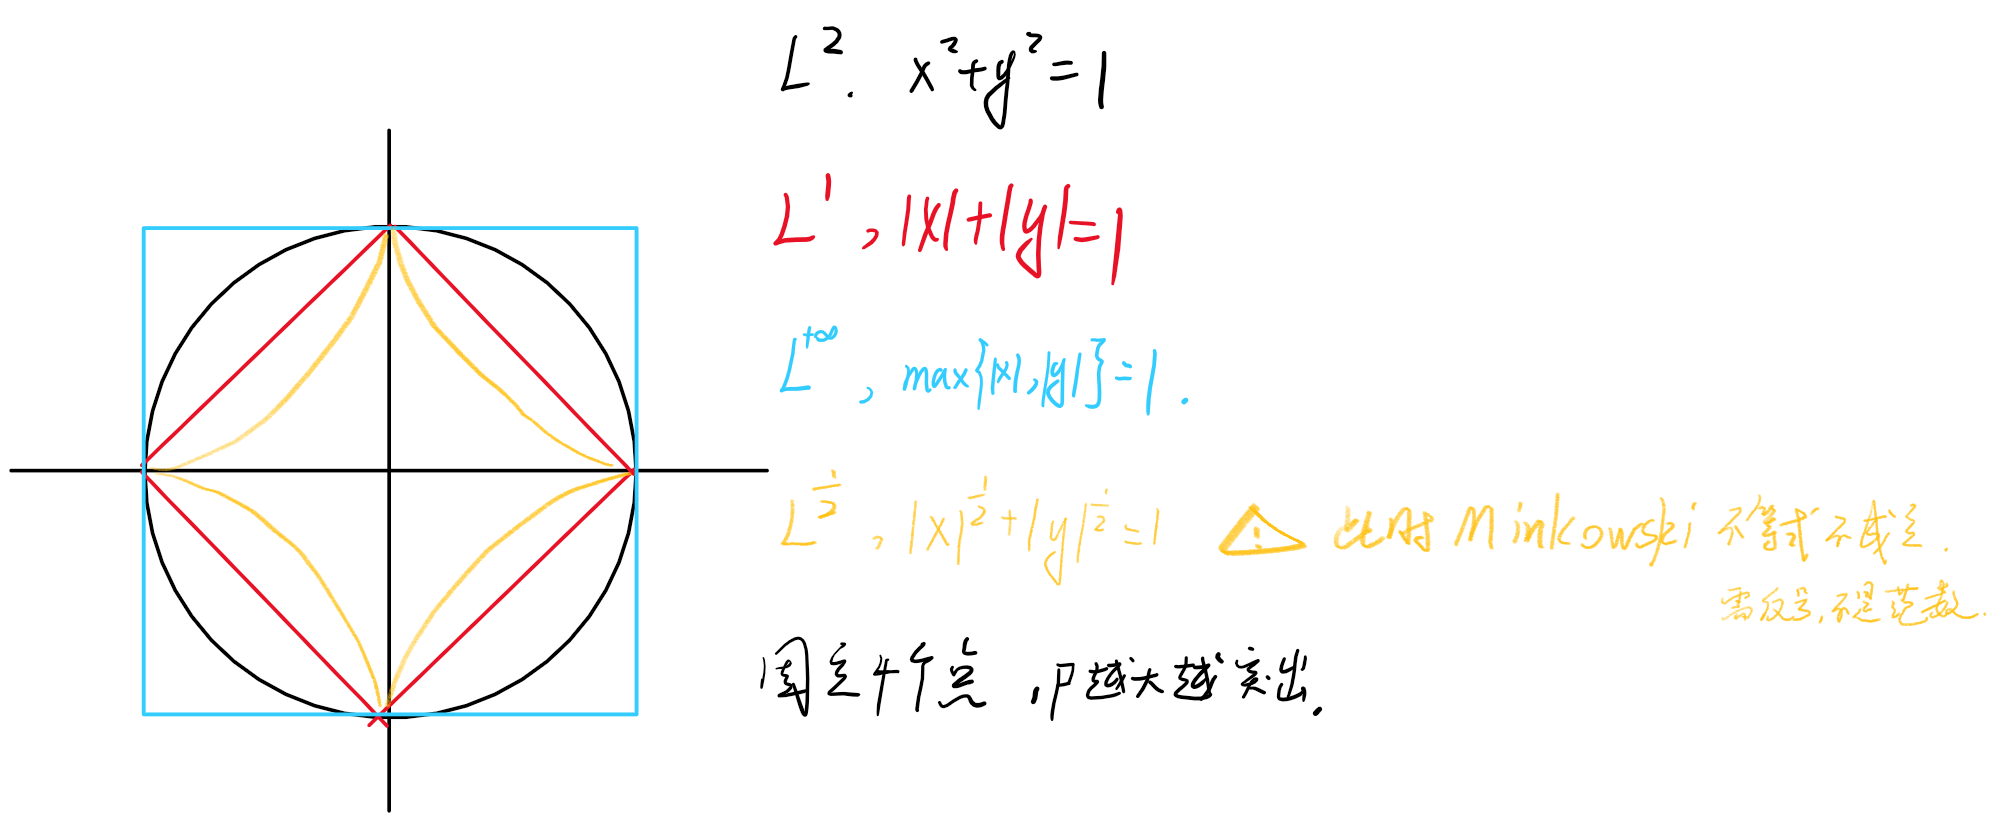
\includegraphics[scale=0.6]{danweiqiu.png}
    \label{fig:1}
  \end{figure}
  特别说明,我这里给出了$P=\frac{1}{2}$的情况,用来说明,对于单位球,其实就是固定4个点,然后P越大曲线越往外凸.
  \subsection{函数空间上的$L^P$范数}
  既然有了Euclide空间上的$L^P$范数,我们自然也会想在其他空间上玩玩这个.最熟悉的空间莫过于函数空间了!
  仿照之前的$L^P$范数,我们发现,不太好给函数又加和又开方什么的.但是所幸我们有一个替代方案,那就是同样非常熟悉的Riemann积分!
  \subsubsection{Définition}
  对$\C ^0I$上的函数$f$,定义范数:
  $$
  \Vert f \Vert_P=(\int_{I}|f(x)|^P \mathrm{d} x)^{\frac{1}{P}},P\ge1
  $$
  这样就得到了函数空间上的$L^P$范数!
  \subsubsection{Remarque}
  我们发现,当$P\rightarrow \infty$时$L^\infty$范数$\Vert f \Vert_\infty=\max|f(x)|,x\in I$,这正是函数$f$在$I$上的上确界.
  现在回顾之前我们对一致收敛的定义,那里提到的$\Vert f_n-f \Vert_\infty\rightarrow 0$就非常好理解了.
\section{空间的完备化}
  (Introduction)让我们先通过一个例子引出完备空间.
  \subsection{实数:七个等价命题}
  我们说"实数$\R$是完备的",这对应于七个等价的命题.这些命题可以相互推导:
  \begin{itemize}
    \item Dedekind分割定理
    \item 确界原理
    \item Heine-Borel定理
    \item 单调收敛定理
    \item 闭区间套定理
    \item Bolzano-Weierstrass定理
    \item Cauchy收敛原理
  \end{itemize}
  这其中,AAAAA是本讲义已经介绍过的内容,剩余的(带介绍).

  在这七个命题里,Cauchy收敛原理应为只涉及了度量,故比较容易用来达成我们的完备化步骤.我们将通过这一原理来详细阐述一个度量空间的完备化
  \subsection{收敛}
  当我们尝试把范数、度量、内积等等概念都抽象化、公理化地定义了之后,是时候重新回顾一下,一个重要概念——收敛了.
  当然,课程的内容只在赋范空间内讨论了收敛,所以我们先看赋范空间内的.
  我们会尝试用精确的$\epsilon-\delta$语言来定义它:
  \subsubsection{Définition}
  赋范空间$(E,\Vert \cdot \Vert)$中,点列$(u_n)_{n\in\mathbb{N}},l\in E$,若:
  $$
    \forall\epsilon>0, \exists p\in \mathbb{N}, n\ge p\Rightarrow \Vert u_n-l \Vert<\epsilon
  $$
  称$(u_n)_{n\in\mathbb{N}}$在$(E,\Vert \cdot \Vert)$中收敛于$l$.
  \subsection{Proposition}
  若$(u_n)_{n\in\mathbb{N}}$在$(E,\Vert \cdot \Vert)$中收敛于$l$,则$(u_n-l)_{n\in\mathbb{N}}$在$(E,\Vert \cdot \Vert)$中收敛于$0$.
  \subsection{Proposition}
  若$(u_n)_{n\in\mathbb{N}}$在$(E,\Vert \cdot \Vert)$中收敛于$l_1$和$l_2$,且二者同属于赋范空间$(E,\Vert \cdot \Vert)$,则$l_1=l_2$
  
  
  \subsection{Cauchy列与收敛}
  下面我们进入到度量空间,利用Cauchy列讨论完备.
  \subsubsection{Définition}
  度量空间$(X,d)$中,点列$(u_n)_{n\in\mathbb{N}}$,若:
  $$
    \forall\epsilon>0, \exists p\in \mathbb{N}, m>p,n>p\Rightarrow d(u_m,u_n)<\epsilon
  $$
  称点列$(u_n)_{n\in\mathbb{N}}$是一个Cauchy列.
  \subsubsection{Proposition}
  度量空间中收敛的点列一定是Cauchy列.
  \subsubsection{Proposition}
  度量空间中的Cauchy列一定有界.
  \subsubsection{Proposition}
  子列收敛的Cauchy列一定收敛.


  \subsection{再论闭包与稠密集}
  \subsubsection{闭包}
  现在我们可以尝试把集合拖到赋范空间里,尝试定义集合的闭包.
  对赋范空间$(E,\Vert \cdot \Vert)$中的集合$A$,定义其闭包为:
  $$
    \overline{A}=\{x\in E | \forall(a_n)\in A^\mathbb{N},a_n\xrightarrow[n\rightarrow+\infty]{}x\}
  $$

  \subsubsection{Proposition}
  赋范空间$(E,\Vert \cdot \Vert)$中的集合$A\in\overline{A}$.
  \subsubsection{稠密集}
  对赋范空间$(E,\Vert \cdot \Vert)$和其中的集合$A$,如果:
  $$
    \forall x\in E, \exists (a_n)\in A^\mathbb{N}, a_n\xrightarrow[n\rightarrow+\infty]{}x
  $$
  称集合$A$在$E$上是稠密的.显然,常见的如有理数集在实数集上仍然是稠密的.
  \subsubsection{Bonus}
  Pierre曾在某次作业里要求证明无理数集在$\R$上稠密.当你学了这里的定义之后应该就非常简单了.当时我是这么写的:\\

    Soit $\mathbb{I} =\R\setminus \mathbb{Q}$.
    $\forall x\in \R$:\\
    \indent
    Si $x\in \mathbb{I}$, 
    soit une suit $\left \{ \alpha_n \right \}=x \Rightarrow 
    \lim_{n \to \infty}x=x\in \mathbb{\overline{I}}$.\\
    \indent
    Si $x\in \mathbb{Q}$, 
    soit une suit $\left \{ \beta_n \right \}=x-\frac{\sqrt{2}}{n}$. 
    $\forall n\in \mathbb{N}, \beta_n=x-\frac{\sqrt{2}}{n}\in \mathbb{I}$ et 
    $\lim_{n \to \infty}\beta_n=x\in \mathbb{\overline{I}}$.\\
    \indent
    Donc $\forall x\in \R, \exists (a_n)_{n\in\mathbb{N}}\in \mathbb{I}^{\mathbb{N}}, n\xrightarrow[a_n\rightarrow\infty]{}x$. 
    Cela dit que $\mathbb{I}=\R\setminus \mathbb{Q}$ est dense dans $\R$.\\


  \subsection{完备空间与完备化 }
  \subsubsection{Définition}
  若度量空间$(X,d)$中任意一个Cauchy列都收敛,称度量空间$(X,d)$是完备的(complet)度量空间.
  称完备的赋范空间为Banach空间,完备的内积空间为Hilbert空间.想要熟悉这两个空间的具体性质就去学习泛函分析吧.\\

  把一个度量空间加上其Cauchy列的极限点组成的最小度量空间这一过程称为对度量空间的完备化.例如,有理数集的完备化就是实数集.

\section{等价度量与等价范数 }  \label{myref:normeq}
  \subsection{双Lipschitz条件 }
  给定两个度量空间$(E_1,d_1),(E_2,d_2)$,集合$U\subseteq E_1$.
  若对于函数$f:U\rightarrow E_2$存在常数$K$使得对任意集合$U$中的元素$(a,b)$有:
  $$
  d_2(f(a),f(b))\leq Kd_1(a,b)
  $$
  称该函数符合Lipschitz条件.\\
  若存在$K\ge 1$使得:
  $$
  \frac{1}{K}d_1(a,b)\leq d_2(f(a),f(b))\leq Kd_1(a,b)
  $$
  称该函数符合双Lipschitz条件.
  \subsection{等价范数 La norme équivalente}
  \subsubsection{Définition}
  设线性空间$E$上的两个范数$N_1$和$N_2$若:
  $$
    \exists(a,b)\in(0,+\infty),\forall x\in E,aN_1(x)\leq N_2(x)\leq bN_1(x)
  $$称$N_1$和$N_2$是等价(équivalente)范数.
  \subsubsection{Remarque}
  等价范数是等价关系,具有自反性、传递性和对称性.
  \subsubsection{Proposition}
  n维线性空间上的所有范数等价.

\chapter{内积 Produit Scalaire}
  这一部分是在小学期讲的.
    \subsection{Définition}
    \subsection{Cauchy-Schwatz不等式}
    \subsection{内积诱导的范数}
    \subsection{平行四边形等式}


\chapter{拓扑空间\\ Espace Topologique}
拓扑是什么?拓扑学内容有哪些?拓扑这个词或许经常听到,但是对于具体的含义和内容想必不是很了解.
事实上,从度量开始,就已经可以算是拓扑学的内容了,我们已经学习了好几章的拓扑学,只不过到了这一章才正式地把这些概念定义出来.
之前我们完成了距离的公理化、模长的公理化和内积的公理化,拓扑也是一个我们熟悉的概念公理化,那就是开集.
拓扑研究的就是开集的集族(Famille d'ensembles).
\section{拓扑空间}
  与度量空间、赋范空间和内积空间类似,拓扑也有对应的拓扑空间,定义如下:
  \subsection{Définition}
  给定集合$X$和集族$\tau $,满足:
  $$
  \begin{aligned}&
  1.\varnothing\in\tau , X\in\tau\text{,空集和全集是开集}\\&
  2.\forall\alpha\in I,U_\alpha\in\tau \Rightarrow\bigcup_{\alpha\in I}U_\alpha\in\tau \text{,开集的并集是开集.}\\&
  3.\forall n\in\mathbb{N},\bigcap_{i=1}^{n}U_i\in\tau \text{,开集的有限交是开集.}\\
    \end{aligned}
  $$
  则称$\tau $是$X$上的一个拓扑,称$(X,\tau)$是一个拓扑空间,$U$称其中的开集.
  \subsection{Remarque:其他的公理化}
  除了以上的公理化方式,还有两种常见的拓扑定义.
  \subsection{Proposition:闭集}
  由de Morgan定律得:
  $$
  \begin{aligned}&
  1.\varnothing, X{ 是闭集.}\\&
  2.\forall\alpha\in I,E_\alpha\text{是闭集} \Rightarrow\bigcap_{\alpha\in I}E_\alpha \text{是闭集.闭集的交是闭集.}\\&
  3.\forall n\in\mathbb{N},\bigcup_{i=1}^{n}E_i \text{是闭集.闭集的有限并是闭集.}\\
    \end{aligned}
  $$
  \subsection{Exemple}
  $\R$上的所有形如$[a,b)$的区间可以组成一个拓扑,其中每个$[a_i,b_i)$都是开集.

  \subsection{离散拓扑 Topologie discrète}
  离散拓扑即$\tau=\mathcal{P} (X)$,其拓扑是集合的幂集,也就是其所有子集的集族.
  离散拓扑空间里所有的单点集都既是开集又是闭集,相互之间都是"孤立的".

  \subsection{密着拓扑 Topologie grossiète}
  密着拓扑即$\tau=\{X,\varnothing \}$,又叫不可分拓扑,其空间里只有空集和整个空间是开集,所有的点都被"粘在一起",无法通过拓扑的方式区分开来.\\
  
  可以认为,离散拓扑和密着拓扑是两个"极端的"拓扑,全包和全不包.
  也正因为其极端性,它们有着一些特殊的性质,我们在后续研究.
  
  \subsection{度量诱导的拓扑}
  对$(X,\tau)$,若存在度量$d$可以定义拓扑的开集,称$(X,\tau)$是可度量的(英:metrizable).
  例如,\prettyref{myref:lisanduliang}的离散度量可以诱导离散拓扑,此时邻域$N_\frac{1}{2}=\{X\}$就是开集.
  而对于card$(X)>1$的密着拓扑就无法被度量.
  \subsection{有限补拓扑 Topologie des compléments finis}
  有限补拓扑中,补集有限的集合是开集.即$\tau=\{U|U\subseteq X,U^C\text{是有限集} \}\cup \{\varnothing\}$

  \subsection{子空间拓扑}\label{myref:soustopo}
  提前预告一下,这是个简单但是非常重要的概念,我们在后面的证明中会多次用到这个概念.\\
  对$(X,\tau)$,$Y$是$X$的子集,则存在一个拓扑$\tau_y=\{Y\cap U| U\in\tau\}$,也就是说,拓扑与子集的交集可以组成一个新的拓扑.
  \subsubsection{Démonstration}
  $$
  \begin{aligned}&
  \varnothing\cap Y=\varnothing\in\tau_y\\&
  X\cap Y=Y\in\tau_y\\&
  \bigcup_{\alpha\in I}(U_\alpha\cap Y)=(\bigcup_{\alpha\in I}U_\alpha)\cap Y\in Y\\&
  \bigcap^n_{i=1}(U_i\cap Y)=( \bigcap^n_{i=1}U_i)\cap Y\in Y
  \end{aligned}
  $$
  \subsubsection{Exemple}
  对于$\R$上的常规拓扑和子集$Y=[0,+\infty),\forall (a,b)\in\R,(a,b)\cap[0,\infty)\in\tau_y$.
\section{拓扑空间里的点集}
  现在让我们来看一看那些以前很熟悉的概念拿到拓扑空间里之后会发生什么.
  \subsection{邻域}
  对$(X,\tau)$中的一点$x$,若存在开集$U\in\tau, x\in U$,则称$U$是$x$的一个邻域,记为$U(x)$,$U/x$是$x$的去心邻域,记为$\check{U}(x) $.
  注意到,现在的邻域跟之前的在对称性上有所差异,之前我们规定一个点的邻域好像都是关于这个点"对称"的,点在邻域的正中央,现在这个点可以在邻域里的任意位置.
  我当初学到这里也觉得奇怪,但是后面一想,也没用上这个所谓的对称性啊,所以其实问题不大.
  \subsection{内点}
  $(X,\tau), E\subseteq X,x\in E,\text{若存在} U(x)\subseteq E$则称呼$x$是$E$的一个内点. $E$的所有内点组成的集合称为其内部,记为$E^O$.
  \subsection{极限点与闭包点}
  $(X,\tau), E\subseteq X,x\in E$若有$\forall\check{U}(x)\cap E\neq\varnothing$,则$x$是$E$的极限点.$E$的所有极限点组成的集合称为导集,记为$E'$.同理,
  若有$\forall U(x)\cap E\neq\varnothing$,则$x$是$E$的闭包点.$E$的所有闭包点组成的集合称为闭包,记为$\bar{E}$.
  熟悉的感觉又回来了.同样,我们可以证明$\bar{E}=E\cup E'$.
  \subsection{外点与边界点}
  与内点这个概念相对应,考虑$E$的补集$E^C$,将其内点称为$E$的外点,组成的集合称为外部,记为$E^e$.不是内点又不是外点的点称为边界点,组成的集合称为边界,记为$\partial E$.
  \subsection{熟悉的命题}
  把以前的一些命题拿过来放到拓扑空间,它们仍然成立.
  \begin{itemize}
    \item $U\text{是开集}\Leftrightarrow U=U^O$,内部等于自身的集合是开集.
    \item $U^O=(U^O)^O$,内部是开集.
    \item $U^O$是包含于$U$的最大开集.
    \item $E\text{是闭集}\Leftrightarrow E=\bar{E}$,闭包等于自身的集合是闭集.
    \item $\bar{E}=\bar{\bar{E}}$,闭包是闭集.
    \item $\bar{E}$是包含于$E$的最小闭集.
  \end{itemize}
  \subsubsection{Démonstration}
  待补充,笔记上的太乱了.




\section{拓扑空间里的收敛 }
  现在我们要在拓扑空间中再次研究这个重要的,贯穿了大量分析学内容的概念————收敛.
  \subsection{Définition}
  $(X,\tau)$中的点列$\{a_n\}$和一点$x$,若有:
  $$
  \forall U(x), \exists N\in \mathbb{N}*\text{使得}n>N\Rightarrow a_n\in U(x)
  $$
  称点列$\{a_n\}$收敛于点$x$.
  \subsubsection{Exemple}
  $X=\{a,b,c\},\tau =\{\varnothing, X, \{a,b\}, \{a,c\}, \{a\}\},a_n\equiv a$.则有$\{a_n\}$收敛于点$a$.
  \subsubsection{Remarque:收敛不唯一}
  注意到,在上述的条件里,点列的收敛是不唯一的!!!因为$\{a,b\}$也是点$a$的邻域,所以$\{a_n\}$收敛于点$b$;$\{a,c\}$也是点$a$的邻域,所以$\{a_n\}$收敛于点$c$.也就是说,$\{a_n\}$同时收敛于$a,b,c$三个不同的点!
  这多么可怕,与我们之前见过的只收敛到一个点的收敛概念完全不同.出现这一情况,是因为在之前我们学习的空间里,两个点之间存在没有交集的邻域,但是在拓扑空间里这条法则失效了,所以收敛有了这样的奇怪的性质.
  然而这不是什么好的性质,如果点列的收敛是不唯一的,那我们就无法区分收敛到的哪些点了,点集拓扑的探讨也就失去了意义.
  所以这一个收敛的定义其实不重要,因为没什么用.我们必须对它加以改进,添加更多的限制条件来确保能有效运用收敛.
  \subsection{Hausdorff条件:$T_2$公理}
  对$(X,\tau)$中任意两点$x_1,x_2$,若:
  $$
    \forall(x_1,x_2)\in X^2, x_1\neq x_2, \exists U(x_1),U(x_2)\text{使得}U(x_1)\cap U(x_2)=\varnothing
  $$
  则称$X$是一个Hausdorff空间.该条件又称为拓扑空间里的分离公理,或者$T_2$公理,它把空间里的点分离开了.
  \subsubsection{Proposition}
  一个有限集是一个Hausdorff空间,当且仅当它的$\tau$是离散拓扑.
  \subsubsection{Démonstration}
  离散拓扑的有限集显然是Hausdorff空间.我们证明另一个方向,利用反证法:
  $$
  \begin{aligned}&
    \lnot (\tau\text{是离散拓扑})\Rightarrow \exists x\in X, \{x\}\notin \tau\\&
    \text{设}x \text{的所有邻域交集为}\mathbb{U}\Rightarrow\mathbb{U}\cap x\neq\varnothing \\&
    \text{设}y\in\mathbb{U}\cap x\\&
    \Rightarrow \forall U(y)\cap\mathbb{U}\neq\varnothing\\&
    \Rightarrow \forall U(y),\forall U(x),U(y)\cap U(x)\neq\varnothing\\&
    \Rightarrow X\text{不是Hausdorff空间}
    \end{aligned}
  $$
  所以我们发现,如果研究有限集,那就绕不开离散拓扑,研究其收敛性也就没什么意义了.
  \subsubsection{Proposition}
  Hausdorff空间里点列的收敛具有唯一性,即$\{a_n\}$收敛于点$x$和$y\Rightarrow x=y$.
  \subsection{Hausdorff空间里的闭集}
  Hausdorff空间里单点集都是闭集.
  \subsubsection{Démonstration}
  对于Hausdorff空间里一点$x$,有:
  $$
  \forall y\in x^C, \exists U(y)\cap x\neq\varnothing\Rightarrow U(u)\subseteq x^C\Rightarrow y\in(x^C)^O
  $$因此$x^C$是个开集,那$x$自然就是个闭集了.
  \subsubsection{Proposition}
  Hausdorff空间里有限集都是闭集.
  \subsubsection{Proposition}
  度量空间都是Hausdorff空间.

  \subsection{Fréchet条件:$T_1$公理}
  在证明Hausdorff空间里单点集都是闭集的时候,我们用到了这样一步:
  $$
  \exists U(y)\cap x\neq\varnothing
  $$
  对比Hausdorff条件本身,我们发现这里没有用全.我们只用了点和邻域的关系而不是邻域和邻域的关系,这说明Hausdorff条件是一个很强的条件,我们可以尝试再稍微弱化一下它.
  于是就有了Fréchet条件:单点集都是闭集的拓扑空间称为Fréchet空间.





  \subsection{$T_0$公理与Kolmogorov体系}
  这里重新调整一下

  \section{拓扑公理体系 Systeme d'axiomes topologiques}
  \subsection{$T_0$ Kolmogorov 公理 Axiome de Kolmogorov}
  \subsection{$T_1$ 公理 Axiome de Fréchet}
  \subsection{$T_2$ Hausdorff 公理 Axiome de Hausdorff}
  \subsection{$T_3$ 正规公理 Axiome régulier}
  \subsection{$T_4$ 公理 Axiome complètement régulier}
  \subsection{$T_5$ 公理 Axiome complètement régulier de Hausdorff}
  \subsection{$T_6$ 公理 Axiome dénombrable}
  \subsection{$T_7$ 公理 Premier axiome dénombrable}
  \subsection{$T_8$ 公理 Deuxième axiome dénombrable}
  \subsection{$T_9$ 公理 Axiome de Lindelöf}


\section{连续性与映射}
  现在,我们继续公理化拓扑空间里映射的连续性.
  \subsection{Définition}
  考虑两个拓扑空间$(X,\tau_x)(Y,\tau_y)$上的映射$f:X\rightarrow Y$,若:
  $$
  \forall U\in\tau_y,f_{-1}(U)\in\tau_x
  $$
  则称映射$f$是连续的.
  \subsection{拓扑的选择与连续性}
  对于同一个集合,我们选择不同的拓扑,则可能导致连续性的改变.
  例如,设$\R_d$是$\R$上的离散拓扑,$\R_n$是$\R$上的通常拓扑,$f(x)=x$是恒等映射,则:
  \begin{itemize}
    \item $f:\R_n\rightarrow \R_d$不是连续映射,单点集在$\R_n$上不是开集.
    \item $f:\R_d\rightarrow \R_n$是连续映射.
  \end{itemize}
  \subsection{由公理推导而来的等价命题}
  一下命题等价,它们分别对应着不同的拓扑公理.这也说明拓扑公理是可以相互转化的.
  \begin{itemize}
    \item 1.$\forall U\in\tau_y,f_{-1}(U)\in\tau_x$.(开集公理)
    \item 2.$\forall E\subseteq X,f(\bar{E})\subseteq \bar{f(E)}$.(闭包公理)
    \item 3.$\forall E\in Y\text{是闭集},f_{-1}(E)\in X\text{是闭集}$.(闭集公理)
    \item 4.$\forall x\in X, \forall U[f(x)], \exists U(x)\text{使得}f[U(x)]\subseteq U[f(x)]$.(邻域公理)
  \end{itemize}
  \subsubsection{Démonstration}
  $1\Rightarrow 2$:
  $$
  \begin{aligned}&
    \forall x\in \bar{E},f^{-1}U[f(X)]\cap E\neq\varnothing\\&
    \Rightarrow U[f(x)]\cap f(E)\neq\varnothing\Rightarrow f(x)\in \bar{f(E)}
    \end{aligned}
  $$


  $2\Rightarrow 3$:
  $$
  \begin{aligned}&
    \forall x\in \bar{f^{-1}(E)},f(x)\in \bar{E}\\&
    \Rightarrow x\in f^{-1}(E)\Rightarrow\bar{f^{-1}(E)}\subseteq f^{-1}(E)\\&
    \Rightarrow f^{-1}(E)\text{是闭集}
    \end{aligned}
  $$


  $3\Rightarrow 1$:
  $$
  \begin{aligned}&
    U\subseteq \tau_y\Rightarrow U^C\text{是闭集}\Rightarrow f^{-1}(U^C)\text{是闭集}\\&
    \Rightarrow f^{-1}(U^C)=[f^{-1}(U)]^C\Rightarrow f^{-1}(U)\in\tau_x
    \end{aligned}
  $$


  $4\Rightarrow 1$:
  这里的证明其实就是前面证明过的东西反过来,留给读者完成.
  \subsection{Exemple}
  接下来给出几个连续映射
  \subsubsection{常值映射 }
  $$
    f:X\rightarrow  Y
  $$
  $$
    x\rightarrow C
  $$
  $\forall \text{开集}U\subseteq Y,C\in U\Rightarrow f^{-1}(U)=X \text{是开集}, 
  C\notin U\Rightarrow f^{-1}(U)=\varnothing \text{是开集}$,故常值映射是连续映射.
  \subsubsection{包含映射 }
  包含映射是$X$的子集$A$上的恒等映射
  $$
    i:A\hookrightarrow  X
  $$
  $$
    x\rightarrow x
  $$
  $\forall \text{开集}U\subseteq X,i^{-1}(U)=U\cap A \text{是开集(子空间拓扑)}$,故常值映射是连续映射.
  \subsubsection{复合映射 }
  给定连续映射$f:X\rightarrow  Y\text{    }g:Y\rightarrow  Z$,其复合映射
  $$
    \phi:X\rightarrow Z
  $$
  $$
    x\rightarrow g(f(x))
  $$
  也是连续映射.$\forall \text{开集}U\subseteq Z,g^{-1}(U)\subseteq Y 
  \text{是开集}\Rightarrow f^{-1}(g^{-1}(U))\subseteq X\text{是开集}\Rightarrow (f\circ g)^{-1}(U)\text{是开集}$,
  故连续映射的复合映射也是连续映射.
  \subsubsection{限制映射 }
  考虑连续映射$f:X\rightarrow Y$,对$A\subseteq X:$
  $$
  f|_A:A\rightarrow Y
  $$
  $$
    x\rightarrow f(x)
  $$
  为连续映射(考虑包含映射和映射$f$的复合映射即可).
  \subsubsection{陪域缩小}
  考虑连续映射$f:X\rightarrow Y$,对$Z\subseteq X:$
  $$
    f': X\rightarrow Z
  $$
  $$
    x\rightarrow f(x)
  $$
  则$f'$也是连续映射(考虑映射$f$和包含映射的逆映射的复合映射即可).
  \subsubsection{陪域扩大}
  考虑连续映射$f:X\rightarrow Y$,对$Y\subseteq Z:$
  $$
    f': X\rightarrow Z
  $$
  $$
    x\rightarrow f(x)
  $$
  则$f'$也是连续映射(考虑映射$f$和包含映射的复合映射即可).
  \subsection{局部表示与粘接原理 }
  在讨论拓扑空间上的连续函数时,我们不必要求直观地看出整个函数都是连续的,而是可以间接地"拼凑"出一个连续函数.
  若我们采用开集"拼凑",则这个过程称为连续性的局部表示;若采用闭集,则称为粘接原理.即对拓扑空间上的函数$f:X\rightarrow Y$:
  $$
    X=\bigcup_{\alpha\in I}U_\alpha ,\forall \alpha\in I, U_\aleph\text{是开集}
  $$
  $$
  \forall \alpha\in I,f|_{U_\alpha}:U_\alpha\rightarrow Y\continue\Rightarrow f:X\rightarrow Y\continue
  $$
  即为连续性的局部表示;
  $$
    X=\bigcap_{i=0}^{n}V_i ,\forall i\in[\![0,n]\!], V_i\text{是闭集}
  $$
  $$
    \forall i\in[\![0,n]\!],f|_{V_i}:V_i\rightarrow Y\continue\Rightarrow f:X\rightarrow Y\continue
  $$
  \subsubsection{Démonstration}
  \begin{figure}[H]%插入题目的图片
    \centering
    
\includegraphics[scale=0.2]{proofforreader.jpg}
  \end{figure}


\section{同胚 Homeomorphisme}\label{myref:tongpei}
  现在我们来到了拓扑里面最重要的概念——同胚.你可能听过这个著名的笑话:\\

  一个拓扑学家把咖啡倒进了甜甜圈里.有人问他为什么不把咖啡倒进咖啡杯里,拓扑学家非常惊讶:"它们有什么区别?不是同胚的吗?"
  \subsection{Définition}
  对拓扑空间上的映射$f:X\rightarrow Y$若$f$满足:
  \begin{itemize}
    \item $f$是双射
    \item $f$是连续映射
    \item $f^{-1}$是连续映射
  \end{itemize}
  则称$f$是$X$到$Y$上的一个同胚映射,此时$X$和$Y$是同胚的.显然,同胚是一个等价关系.
  \subsection{Exemple}
  \subsection{Remarque}
  请回顾我们在\prettyref{myref:Homomorphisme}和\prettyref{myref:Isomorphisme}里提到的同态和同构,它们有什么相似的地方?\\

  在拓扑空间上前两条无法推出第三条性质,我们讲马上给出一个经典的反例用来说明这一点.
  \subsection{Exemple: 反例}
  给出由半开半闭区间$[0,1)$到单位圆上的映射
  $$
  f:[0,1)\rightarrow \{(x,y)|x^2+y^2=1\}
  $$
  $$
  x\mapsto\cos(2\pi x)+\sin(2\pi x)
  $$
  $f$是连续的双射,但是$f^{-1}$在$(1,0)$处不连续.
  这是因为我们把区间的两端"粘贴"了起来,这导致了拓扑性质的改变,因此无法保持同胚.事实上,只要进行了类似"粘贴""裁剪"或者"穿孔"等等操作,原来的拓扑就变了.
  这些操作会在拓扑学里严格定义,这里不再谈论.
  \subsection{Proposition}
  对$\R$上的一元函数$f:X\rightarrow Y$,有:$X,Y$是$\R$上的两个区间(不能是子集!).若:
  \begin{itemize}
    \item $f$是双射
    \item $f$是连续映射
  \end{itemize}
  则$X,Y$同胚.
  \subsection{Exemple: 反例}
  若上述推论里将\textbf{$X,Y$是$\R$上的两个区间} 改成 \textbf{$X,Y$是$\R$上的两个子集} ,则结论不成立.
  例如映射$f:X\rightarrow Y$有 $X=[0,1]\cup(2,3],Y-[0,2]$
  $$
  x\mapsto 
  \begin{cases}
    x &x\in[0,1]\\
    x-1 &x\in (2,3]
    \end{cases}
  $$
  则$f^{-1}$不连续.
  \subsection{Proposition}
  对双射$f:X\rightarrow Y$,若:
  $$
  U\text{是$X$上的开集}\Leftrightarrow f(U)\text{是$Y$上的开集}
  $$
  则$X,Y$同胚.

  \section{紧致性与列紧性 Compacité et séquentialité}
  \subsection{拓扑不变量 Topological invariant}
  与同构类似,同胚的拓扑空间也有一些不会变化或者相等的东西.这些东西被称为拓扑性质或者拓扑不变量.
  它们在同胚映射下保持不变.由于许多概念还没有讲到,我们仅仅给出拓扑不变量的概念,以便于大家理解拓扑空间上的紧致性.
  更多的拓扑不变量将在拓扑学中研究.
  \subsection{Remarque}
  我们将以前所学过的度量空间上的开覆盖推广到拓扑空间.这并没有难度,因为拓扑空间直接就是拿开集定义的,不需要额外添加什么内容.
  对拓扑空间$X$上的开集族$\{U_\alpha|\alpha\in I \}$满足
  $$
    X\subseteq \bigcup_{\alpha\in I}U_\alpha
  $$则称$\{U_\alpha\}$是拓扑空间$X$上的一个开覆盖.\\

  同理,若能找到一组有限个开集覆盖$X$,即A和B拥有相同的基数
  $$
  X\subseteq \bigcup_{i=1}^{n}U_i
  $$则称$\{U_\alpha\}$是拓扑空间$X$上的一个有限开覆盖/有限子覆盖.
  \subsection{Définition: 紧致}
  对拓扑空间$X$上的任意一个开覆盖,若都能找到一个有限子覆盖,则称$X$是一个紧致空间,或称$X$是紧的.
  若$Y\subseteq X$也是紧的,则称$Y$是一个紧致集/紧集.
  \subsection{Définition: 序列紧致}
  对拓扑空间$X$上的任意一个序列,若都能找到一个子序列$\{ x_n\}$收敛于$x\in X$,则称$X$是一个序列紧致空间,或称$X$是列紧的.
  若$Y\subseteq X$也是列紧的,则称$Y$是一个列紧集.
  \subsection{Remarque}
  或许你还记得我们在度量空间上讨论的紧致性问题,当时我们并没有这么区分紧和列紧.
  事实上,在度量空间上,紧致性和列紧性是等价的,这两个概念都起源于Bolzano对于收敛子列的研究.
  在研究收敛性上,发展出了Bolzano-Weierstrass定理和Arzela-Ascoli定理等对于序列紧致性的结论;
  在研究连续性上,又发展出了Heine-Borel定理作为连续性的结论.
  早期的列紧性比紧致性更为直观(显然,度量下的点列收敛肯定比开集更加容易直观理解),因此Fréchet将现在的列紧性定义为紧致.
  但是后来随着拓扑空间研究的深入,人们发现两者不等价,且在拓扑空间上Heine-Borel利用开区间表示的紧致性更容易理解,更何况在一般的拓扑空间下无法讨论序列的收敛,
  因此最终由Pavel和Urysohn用Heine-Borel的方法定义紧致性,而将Bolzano-Weierstrass的方法定义为列紧性.在本章中,我们主要考虑紧致性的问题.
  \subsection{Proposition}
  $Y$是$X$上的一个紧致集等价于以下表述:
  $$
  \text{对开集族 }\{U_\alpha\}\subseteq X, \{U_\alpha\}\text{是 }Y\text{的开覆盖 }\Rightarrow
  \exists\{U_i|i\in[\![1,n]\!]\}\subseteq\{U_\alpha\}\text{是 }Y\text{的有限子覆盖 }
  $$
  这说明了一个很重要的结论:集合的紧致性与其在什么空间上无关.一个紧的$Y$放在任何$X$里都是紧的.
  \subsection{Exemple}
  \subsubsection{1.  $\R$既不紧,也不列紧}
  我们可以找到开覆盖
  $$
  C=\{(n,n+2)|n\in\mathbb{Z}\}
  $$
  从中拿去任意一个区间之后就无法覆盖$\R$了.\\
  对于$\R$趋近于正无穷的子列显然不收敛于$\R$上的某个点.
  \subsubsection{2.  $(0,1]$既不紧,也不列紧}
  \subsubsection{3.  $\{0\}\cup \{\frac{1}{n}|n\in\mathbb{N}\}$既紧,也列紧}
  \begin{figure}[H]%插入题目的图片
    \centering
    
\includegraphics[scale=0.2]{proofforreader.jpg}
  \end{figure}
  \subsection{紧集的投影}
  定义投影算子$\mathcal{P}:X^2\rightarrow X$
  $$
  (a,b)\mapsto a
  $$
  若$A^2$紧致,则$\mathcal{P}(A)$也紧致.
  \subsection{Proposition}
  两个紧集的笛卡尔积同样是紧集.
  $$
  A\times B\text{是紧集}\Leftrightarrow A\text{是紧集}\land B\text{是紧集}
  $$
  \subsection{Proposition}
  有限个紧集的笛卡尔积同样是紧集.(此时不能反推)
  $$
  A_1,\dots,A_n\text{是紧集}\Rightarrow A_1\times \dots\times A_n\text{是紧集}
  $$
  \section{闭集刻画的紧致集}
  利用闭集刻画紧致集,可以在一定程度上简化我们的计算和证明.
  \subsection{Remarque: 有限交性质}
  对集合$X$,设子集族$C=\{U_\alpha|\alpha\in I \}$,若对$C$的任一\textbf{有限}子集族$C_U=\{U_1,U_2,dots,U_n\}$,都有
  $$
  \bigcap_{i=1}^n U_i\neq \varnothing
  $$
  则称$C$具有\textbf{有限交性质}.
  \subsection{Proposition}
  \noindent
  $X$是紧集等价于以下陈述:\\
  对$X$中任意具有有限交性质的闭集族$\{V_\alpha|\alpha\in I\}$,有
  $$
    \bigcap_{\alpha\in I}V_\alpha\neq\varnothing
  $$
  \subsubsection{Démonstration}
  利用De Morgan定律和反证法.
   
  \subsection{Proposition}
  紧致空间内的任意闭子集都是紧集.
  \subsubsection{Démonstration}
  设$Y\subseteq X$,取$Y$的开覆盖$C=\{U_\alpha|\alpha\in I \}$,令$C'=C\cup Y^\complement$,
  则$C'$是$X$的一个开覆盖.若$X$是紧致的,设其有限子覆盖$D=\{U_1,U_2,dots,U_n\}\subseteq C'$.则有:
  $$
  Y^\complement\nsubseteq D\Rightarrow D\text{是}Y\text{的有限开覆盖}\Rightarrow Y\text{是紧集}
  $$
  $$
  Y^\complement\subseteq D\Rightarrow D\setminus Y^\complement \text{是}Y\text{的有限开覆盖}\Rightarrow Y\text{是紧集}
  $$
  \subsection{Proposition}
  Hausdorff空间里紧致集都是闭集
  \subsubsection{Démonstration}


  \subsubsection{Exemple: 反例}
  以上命题不可反推.例如考虑到非Hausdorff空间上$\R$的有限补拓扑,任意的闭集都是紧集,但是也是有限集.

  \section{同伦 Homotopie}
  \section{拓扑不变量 Topologie invariante}
  \section{连通集 Connexité}


\part{代数与矩阵\\ Algèbre et Matrice}
\chapter{线性空间 \\Espace Vectoriel}

\chapter{多项式理论\\ Théorie des Polynômes}
\chapter{矩阵 \\ Matrice}
\chapter{矩阵的简化\\Reduction}
\section{特征值与特征向量 Vecteurs Propres et Valeurs Propres}
  在线性空间中,有一些有趣的线性变换(线性算子)和向量.这些向量经过这些变换前后都处在同一条直线上,仅仅是改变了长度或方向.
  能使向量拥有这种特质的线性变换往往也有许多优秀的性质可以研究,也就是本章的重点.\\
  
  对于这些经过变换前后都处在同一条直线上的向量,称其为对应线性变换的特征向量(le vecteur vropre),
  变换后改变的方向与大小所对应的标量称为线性变换的特征值(la valeur propre),
  将具有相同特征值的特征向量与一个同维数的零向量组成一个集合,称为线性变换的特征空间(l'espace propre).
  \subsection{Définition}
  设$n\in\mathbb{N} , M\in \mathcal{M}_n(\mathbb{K})$.
  若存在$x\in \mathcal{M}_{n,1}(\mathbb{K})\setminus\{0\}, \lambda\in\mathbb{K}$使得:
  \begin{equation}
    \notag
    Mx=\lambda x
  \end{equation}
  则称$\lambda$为矩阵$M$的特征值,$x$为矩阵$M$的特征向量,
  $E_\lambda=\{x\in\mathcal{M}_{n,1}(\mathbb{K})\}$为矩阵$M$的特征空间,
  称特征值集$\sigma_{\mathbb{K}}(M)$为矩阵$M$的谱(le spectre).\\

  若$E$是域$\mathbb{K}$上的线性空间,自同态$u\in \mathcal{L} (E)$,同理
  若存在$x\in E\setminus\{0\}, \lambda\in\mathbb{K}$使得:
  \begin{equation}
    \notag
    u(x)=\lambda x
  \end{equation}
  则称$\lambda$为矩阵$M$的特征值,$x$为矩阵$M$的特征向量,
  $E_\lambda=\{x\in E\}$为矩阵$M$的特征空间,
  称特征值集$\sigma_{\mathbb{K}}(M)$为矩阵$M$的谱.事实上,如果$E$是有限维空间,两种定义是等价的.
  \subsubsection{Remarque}
  还记得\prettyref{myref:tezheng}介绍的“特征”的概念吗?想一下我们为什么要管这里的$\lambda$叫“特征”值.
  \subsection{Proposition:特征空间的性质}
  \subsubsection{线性子空间}
  $E_\lambda$是一个线性子空间(sous-espace vectoriel),满足:
  \begin{equation}
    \notag
    E_\lambda:
    \begin{cases}
    \lambda_i+\lambda_j\in E_\lambda \\
    m\lambda_i\in E_\lambda \\
    E_\lambda\neq \varnothing 
    \end{cases}
  \end{equation}
  \subsubsection{核空间}
  $E_\lambda$是$M-\lambda I_n$的核空间,即:
  \begin{equation}
    \notag
    E_\lambda=\ker(M-\lambda I_n)=\{x|(M-\lambda I_n)x=0_n\}
  \end{equation}
  \subsubsection{非零维度}
  根据特征空间的定义,其至少包含一个非0向量,故$\dim E_\lambda \ge 1$.


\section{特征多项式 Polynôme caractéristique}
  当我们知道了特征值和特征向量,自然就会想问:如何找到矩阵的特征值和特征向量呢?
  随机抽向量和数一个一个计算显然不可能.为了更加便捷,我们需要通过特征多项式来寻找特征值和特征向量.
  \subsection{Définition}
  设$n\in\mathbb{N} , M\in \mathcal{M}_n(\mathbb{K})$,有:
  \begin{equation}
    \notag
    \chi _M(X)=\det(XI_n-M)\footnote{
      需说明的是,许多教材里把特征多项式定义成$\det(M-XI_n)$,计算时需注意反号.两种形式并不影响各种结论.
    }
  \end{equation}
  称$\chi _M(X)$为矩阵$M$的特征多项式.
  显然,我们可以找到$\exists(a_0,...,a_{n-1})\in\mathbb{K}^n$使得:
  \begin{equation}
    \notag
    \chi _M(X)=X^n+\sum_{k=0}^{n-1}a_kX^k
  \end{equation}
  这就是一般的特征多项式的形式.并且,特征多项式的解即为矩阵的特征值.
  一般而言,对布于任何交换环上的方阵都能定义特征多项式.
  \subsubsection{Démonstration}
  \begin{equation}
    \notag
    \begin{aligned}
    & \chi _M(\lambda)=\det(\lambda I_n-M)=0\\
    & \Rightarrow \ker(M-\lambda I_n)\neq\{0\}\\
    & \Rightarrow (M-\lambda I_n)x=\{0\}\\
    & \Rightarrow \lambda\in\sigma_{\mathbb{K}}(M)\\
    \end{aligned}
  \end{equation}
  \subsection{Remarque:域上的特征值}
  在计算矩阵特征值时必须考虑域$\mathbb{K}$的限制.同一个矩阵在不同的域上可能有不同的谱.例如:
  $$
  \begin{aligned}
    R=\begin{pmatrix} 0 & -1 \\ 1 & 0 \end{pmatrix}\\
  \end{aligned}
  $$
  有特征多项式$\chi _R(X)=X^2-1$:\\
  若在实数域上$R\in \mathcal{M}_2(\R)$则$\sigma_{\R}(R)=\varnothing$,\\
  若在实数域上$R\in \mathcal{M}_2(\mathbb{C})$则$\sigma_{\mathbb{C}}(R)=\{i,-i\}$.
  \subsection{二阶特征多项式}
  对二阶矩阵$\mathcal{M}_2(\mathbb{K})$,特征多项式可以简化为:
  $$
  \chi _R(X)=X^2-\mbox{tr}(M)X+\det(M)
  $$
  \subsection{秩为1的自同态}
  对自同态$u\in\mathcal{L} (\R^n)$,若$u$的秩为1,则特征多项式可以简化为:
  $$
  \chi _u(X)=X^{n-1}(X-\mbox{tr}(u))
  $$
  \subsection{多项式的分裂域}
  本节只对分裂域(根域)作简单介绍,详细内容过于复杂,不在本课程讨论范围内.
  在抽象代数中,一个系数域为$\mathbb {K}$ 的多项式${P(x)}$的分裂域(根域)是
  $\mathbb {K} $的“最小”的一个扩域$\mathbb{L}$,
  使得在其中$P(x)$可以被分解为一次因式$x-r_{i}$的乘积,
  其中的$r_{i}$是$\mathbb{L}$中元素.
  一个$\mathbb {K} $上的多项式并不一定只有一个分裂域,
  但它所有的分裂域都是同构的,也就是在同构意义上,$\mathbb {K} $上的多项式的分裂域是唯一的.
  \subsubsection{Définition}
  若存在$(c,\alpha_1,\dots,\alpha_n)\in\mathbb{K}^{n+1}$使得:
  $$
    P(X)=c\prod_{i=1}^{n} (X-\alpha_i)
  $$
  称$P$在$\mathbb {K} $上是分裂的(scindé).这意味着$P$所有的根都在$\mathbb {K} $上.为了更好地理解分裂域,我们举几个例子:
  \subsubsection{Exemple 1}
  $$
    P(X)=(X^2-2)
  $$
  $P$在$\mathbb {R} $和$\mathbb {C} $上都可分裂成$P(X)=(X+\sqrt{2})(X-\sqrt{2})$.
  \subsubsection{Exemple 2}
  $$
    Q(X)=(X^2+4)
  $$
  $Q$在$\mathbb {C} $上可分裂成$Q(X)=(X+2i)(X-2i)$,但是在R上不可分裂.
  \subsection{代数重数La multiplicité}
  在一些地方可能会遇到如下的表示方法:"一个矩阵A的特征值为4,4,3,3,3,2,2,1."
  事实上,我们可以直接得出A的特征值是\{4,3,2,1\},那为什么要对数字进行重复呢?
  根据特征多项式的解法,很容易猜测,重复的次数就是特征值作为根出现的次数,也即代数重数.
  \subsubsection{Définition}
  设多项式$P\in\mathbb {K} [X], \alpha\in\mathbb {K}$,若存在$Q\in\mathbb {K} [X]$使得
  $$
    P(X)=(X-\alpha)^mQ(X)\mbox{且}Q(\alpha)=\neq 0
  $$
  称$m$为根$\alpha$的代数重数.在特征多项式中,记特征值$\lambda$的代数重数为$\mu(\lambda)$.
  \subsubsection{Exemple 1}
  $$
  P(X)=(X-1)^{14}-(X-51)^4
  $$
  其中根1的代数重数为14,根51的代数重数为4.
\section{相似矩阵 Matrice semblable}
  \subsection{Définition}
  设$A$和$B$都属于域$\mathbb {K}$ 上的\n 阶方阵,即$\mathcal{M}_n(\mathbb{K})$.
  若存在$P\in\mathcal{G} \mathcal{L} _n\mathbb{K}$使得:
  $$
    A=PBP^{-1}
  $$
  称$A$和$B$是相似的(semblable).易知相似是一种等价关系.
  \subsubsection{Remarque}
  嘿!还记得\prettyref{myref:conjugaison}提到的共轭关系吗?这就是共轭关系在矩阵里的应用!
  \subsection{Proposition:相似矩阵的特征多项式相等}
  设$A$和$B$是相似矩阵,$\chi_A(X)$和$\chi_B(X)$分别是他们的特征多项式,则有:
  $$
  \chi_A(X)=\chi_B(X)
  $$
  \subsubsection{Démonstration}
  $$
  \begin{aligned}
  &  \chi _A(X)=\det(XI_n-A)=\det(XI_n-PBP^{-1})=\det(XPI_nP^{-1}-PBP^{-1})\\
  &  =\det(P(XI_nP^{-1}-BP^{-1}))=\det(P(XI_n-B)P^{-1})\\
  &  =\det(P)\det(XI_n-B)\det(P^{-1})\\
  &  =\det(XI_n-B)=\chi _B(X)
    \end{aligned}
  $$
  \subsubsection{Proposition}
  若$A$和$B$是相似矩阵,则同理有$\sigma_{\mathbb{K}}(A)=\sigma_{\mathbb{K}}(B)$
  \subsection{Remarque:特征多项式相等不一定相似}
  
  \begin{equation}
    \notag
    A=\begin{pmatrix} 1 & 1 \\ 0 & 1 \end{pmatrix}
    B=\begin{pmatrix} 1 & 0 \\ 0 & 1 \end{pmatrix}
  \end{equation}
  两者的特征多项式都是$(X-1)^2$但明显二者无法相似转化.
  \subsection{Proposition}
  几何重数小于等于代数重数.
  称特征值$\lambda$对应特征空间$E_\lambda$的维数$\dim E_\lambda$为该特征值的几何重数,则有:
  $$
    \forall\lambda\in\sigma_{\mathbb{K}}(M), \dim E_\lambda\leq\mu\lambda
  $$


  如果将代数重数视为一种维数,即它是相应广义特征空间的维数,也就是当自然数k足够大的时候矩阵$(\lambda I_n-A)^k$的核空间.
  也就是说,它是所有“广义特征向量”组成的空间,其中一个广义特征向量满足如果$(\lambda I_n-A)$作用连续作用足够多次就“最终”会成为零向量.
  任何特征向量都是一个广义特征向量,因此任一个特征空间都被包含于相应的广义特征空间.
  这给了一个几何重数总是小于或等于代数重数的简单证明.
  \subsubsection{Démonstration}
  暂略,写不动了,休息一会.
\section{对角化 Diagonalisation}
  \subsection{对角矩阵 Matrice diagonale}
  \subsubsection{Définition}
  设矩阵$A=(a_{i,j})_{(i,j)\in[\![1,n]\!]}\in\mathcal{M}_n(\mathbb{K})$,若:
  $$
    \forall(i,j)\in[\![1,n]\!], i\neq j\Rightarrow a_{i,j}=0
  $$
  称矩阵$A$是对角矩阵.
  记$\mbox{Diag}_n(\mathbb{K})$为$\mathcal{M}_n(\mathbb{K})$上的对角矩阵组成的集合.
  \subsubsection{Exemple}
  $$
  A=\begin{pmatrix} 114 & 0 & 0 \\ 0 & 514 & 0 \\ 0 & 0 & 0 \end{pmatrix}
  $$
  $A$是$\mathcal{M}_3(\R)$上的对角矩阵.
  \subsection{可对角化的 Diagonalisable}
  \subsubsection{Définition}
  对于$\mathcal{M}_n(\mathbb{K})$上的矩阵$M$,
  若存在$(D,P)\in\mbox{Diag}_n(\mathbb{K})\times\mathcal{G} \mathcal{L} _n(\mathbb{K})$使得
  $$
  M=DPD^{-1}
  $$
  则称矩阵$M$是可对角化的.
  \subsubsection{对角化 diagonaliser}
  对一个矩阵$A$,对角化意味着给出一组$(D,P)\in\mbox{Diag}_n(\mathbb{K})\times\mathcal{G} \mathcal{L} _n(\mathbb{K})$.\\

  对一个自同态$u$,对角化意味着给出$E$中的一组基$\mathcal{B}$,使得在这组基下自同态对应的矩阵是对角矩阵.
  \subsection{直和 La somme directe}
  \subsubsection{子空间的和}
  设$F_1,\dots,F_p$是域$\mathbb{K}$上线性空间$E$的一组子空间.其和:
  $$
  F_1+\dots+F_p
  $$
  表示所有$x$组成的集合,其中:
  $$
  \exists(x_1,\dots,x_p)\in F_1\times\dots\times F_p, x=\sum_{i=1}^{p}x_i
  $$
  \subsubsection{Définition}
  设$F_1,\dots,F_p$是域$\mathbb{K}$上线性空间$E$的一组子空间.对任意$x\in(F_1+\dots+F_p)$,若:
  $$
    \exists!(x_1,\dots,x_p)\in F_1\times\dots\times F_p,  
    x=\sum_{i=1}^{p}x_1
  $$
  称这组子空间直和,记为:
  $$
    \bigoplus _{i=1}^pF_i=F_1\oplus\dots\oplus F_p
  $$
  \subsubsection{Exemple}
  \begin{equation}
    \notag
    e_1=\begin{pmatrix} 1 \\ 0 \\ 0 \end{pmatrix}
    e_2=\begin{pmatrix} 0 \\ 1 \\ 0 \end{pmatrix}
    e_3=\begin{pmatrix} 0 \\ 0 \\ 1 \end{pmatrix}
  \end{equation}
  这三个向量张成的空间是直和的,且为$\R^3$.记为:
  $$
  \R^3=\mbox{vect}(e_1)\oplus\mbox{vect}(e_2)\oplus\mbox{vect}(e_3)
  $$
  \subsubsection{Proposition:两个子空间的直和}
  $$
  F_1\oplus F_2 \Leftrightarrow F_1\cap F_2=\{0_E\}
  $$
  \subsubsection{Proposition:直和的维度}
  若$\bigoplus _{i=1}^pF_i=F_1\oplus\dots\oplus F_p$,则有:
  $$
  \sum_{i=1}^{n}\dim(F_i)=\dim(F_1+\dots+F_p)
  $$
  \section{判断可对角化Critères de diagonalisabilité}
  \subsection{特征空间直和}
  设$\mathcal{M}_n(\mathbb{K})$上的矩阵$M$有特征值$\lambda_1,\dots,\lambda_p$,则特征空间直和.即有:
  $$
  \bigoplus _{i=1}^pF_i=E_{\lambda_1}\oplus\dots\oplus E_{\lambda_p}
  $$
  \subsection{自同态的可对角化与直和}
  设$E$是域$\mathbb{K}$上的\n 维线性空间,$u\in\mathcal{L} (E)$,则以下命题等价:
  \begin{flalign*}
    \begin{aligned}
      & \mbox{1.{ }}u\mbox{在域$\mathbb{K}$上可对角化}\\
      & \mbox{2.{ }}E=\bigoplus_{\lambda\in\sigma_{\mathbb{K}}(u)}E_\lambda\\
      & \mbox{3.{ }}n=\sum_{\lambda\in\sigma_{\mathbb{K}}(u)}\dim(E_\lambda)\\
      \end{aligned}
  \end{flalign*}
  \subsection{矩阵的可对角化与直和}
  设$M$是$\mathcal{M}_n(\mathbb{K})$上的矩阵,则以下命题等价:
  \begin{flalign*}
    \begin{aligned}
      & \mbox{1.{ }}M\mbox{在域$\mathbb{K}$上可对角化}\\
      & \mbox{2.{ }}\mathcal{M}_{n,1}(\mathbb{K})=\bigoplus_{\lambda\in\sigma_{\mathbb{K}}(M)}E_\lambda\\
      & \mbox{3.{ }}n=\sum_{\lambda\in\sigma_{\mathbb{K}}(M)}\dim(E_\lambda)\\
      \end{aligned}
  \end{flalign*}
  \subsection{Proposition:势与可对角化}
  设$M$是$\mathcal{M}_n(\mathbb{K})$上的矩阵,
  若$n=\text{card}(\sigma_{\mathbb{K}}(M))$,则$M$可对角化.反之不一定.
  \subsection{对角化过程}
  本节略,主要是一些小技巧.记得先算$\sigma_{\mathbb{K}}(M)$,特征值顺着$D$的对角线往下填.
  再求$E_\lambda$,按特征值的填写顺序排列出$P$,最后求$P^{-1}$即可.在这个过程中,可以从另一个角度理解为什么几何重数小于等于代数重数.、
  如果几何重数大了,$P$就无法按对应的特征值写成一个方阵.



\section{实对称矩阵 Matrice symétrique réelle}
  \subsection{Définition}
  实对称矩阵很好理解,就是矩阵的各个元素都是实数,并且沿着主对角线两端对称.具体定义如下:\\
  对$M\in\mathcal{M}_n(\R)$,若满足:
  $$
  \forall(i,j)\in[\![1,n]\!]^2,\text{{ }}m_{i,j}=m_{j,i}
  $$
  则称$M$为实对称矩阵.显然对于实对称矩阵$M=^\top M$.\n 阶实对称矩阵组成的集合记为$S_n(\R)$.
  \subsection{实特征值}
  实对称矩阵的所有特征值都是实数.
  \subsubsection{Démonstration}
  \begin{flalign*}
    \begin{aligned}
      & Ax=\lambda x\\
      & \Rightarrow ^\top \bar{x} Ax=^\top \bar{x}\lambda x=\lambda^\top \bar{x}x\\
      & \Rightarrow \lambda^\top \bar{x}x=A^\top \bar{x}x=\overline{A^\top \bar{x}x} =A^\top x\bar{x}=\bar{\lambda}^\top x\bar{x}\\
      & \Rightarrow \lambda^\top \bar{x}x=\bar{\lambda}^\top x\bar{x}\\
      & \Rightarrow \lambda=\bar{\lambda}\in\R
      \end{aligned}
  \end{flalign*}
  \subsection{特征向量的正交}
  实对称矩阵不同特征值对应的特征向量相互正交.
  \subsubsection{Démonstration}
  \begin{flalign*}
    \begin{aligned}%怎么输入左上角标?这样打起来很不好看啊
      & ^\top aMb=^{t}(^\top aMb)=^\top b^\top Ma=^\top bMa \Rightarrow ^\top a\lambda_bb=^\top b\lambda_aa\\
      & \Rightarrow \lambda_b\cdot^\top ab=\lambda_a\cdot^\top ba\\
      & \neg(^\top ab=0)\\
      & \Rightarrow \frac{\lambda_b}{\lambda_a}=\frac{^\top ba}{^\top ab}=\frac{^\top (^\top ba)}{^\top ab}=1\\
      & \Rightarrow \lambda_b=\lambda_a\Rightarrow \perp \\
      & \Rightarrow ^\top ab=0
      \end{aligned}
  \end{flalign*}
  

\section{零化多项式 Polynôme annulateur}
  理论上,学习零化多项式之前需要学习矩阵多项式(polynôme de matrice),但是课程中直接将其提了一嘴就省略了.
  实际上这部分内容再本章的应用中也不是特别重要.所以以后有空我再补充相关内容.
  \subsection{Définition}
  设$M\in\mathcal{M}_n(\mathbb{K})$且$P\in\mathbb{K}[X]$,若有:
  $$
  P(M)=0
  $$
  则称多项式$P$是矩阵$M$的零化多项式.
  \subsection{Cayley-Hamilton定理}
  \n 阶方阵$M$的特征多项式就是它的一个零化多项式.即$\chi _M(M)=0$.或写作:
  $$
  \forall\lambda\in\sigma_{\mathbb{K}}(M), P(\lambda)=0
  $$
  记零化多项式的根组成的集合为$\mathcal{Z} (P)$则
  显然有$\sigma_{\mathbb{K}}(M)\subseteq\mathcal{Z} (P)$.
  \subsubsection{Démonstration}
  \begin{flalign*}
    \begin{aligned}
      & Ma=\lambda a,a\neq 0\\
      & P(M)=\sum_{k=0}^{a}a_kM^k=0_n\\
      & \Rightarrow \sum_{k=0}^{a}a_kM^ka=0_{n,1}\\
      & \text{其中,} M^ka=M^{k-1}Ma=\lambda M^{k-1}a=\dots=\lambda^ka\\
      & \Rightarrow \sum_{k=0}^{a}a_k\lambda^ka=0_{n,1}\\
      & \Rightarrow \sum_{k=0}^{a}a_k\lambda^k=0_n\\
      & \Rightarrow  P(\lambda)=0 \\
      \end{aligned}
  \end{flalign*}
  \subsection{相似矩阵的零化多项式}
  \n 阶方阵$A$的特征多项式就是它的一个零化多项式,同理,
  \n 阶方阵$B$的特征多项式也是它的一个零化多项式.
  若$A$与$B$相似,我们知道相似矩阵的特征多项式相等,特征多项式又都是该矩阵的零化多项式,
  自然可以知道,相似矩阵的零化多项式相同.\footnote{
    更多角度和结论可以参考:
    \href{https://zhuanlan.zhihu.com/p/379739220}{https://zhuanlan.zhihu.com/p/379739220}
    }
  \subsection{零化多项式的简单根}
  矩阵$M\in\mathcal{M}_n(\mathbb{K})$可对角化,当且仅当存在一个A的零化多项式可以被分裂得到简单根(racine simple).
  此时零化多项式可以写成:
  \begin{flalign*}
    \begin{aligned}
      & P=\mathbb{K}[X]=\prod_{i=1}^{n}(x-a_i)\\
      & \text{满足:}\\
      & 1.\text{{ }} \forall P(x)=0, x\in\mathbb{K}\\
      & 2.\text{{ }} \forall(a_i,a_j)_{(i,j)\in[\![1,n]\!]^2},a_i\neq a_j
      \end{aligned}
  \end{flalign*}
\chapter{二次曲面 Surface du second degré}
  这里的内容要放到别的地方去,记得修改
  \subsection{Définition}
  从代数的理论中,我们可以证明二次曲面一共具有以下17种.将其分为三大类:
  \subsection{三元二次曲面}
    \subsubsection{椭球面类}
    $$
    \text{椭球面: }\frac{x^2}{a^2}+\frac{y^2}{b^2}+\frac{z^2}{c^2}=1
    $$
    $$
    \text{虚椭球面: }\frac{x^2}{a^2}+\frac{y^2}{b^2}+\frac{z^2}{c^2}=-1
    $$
    $$
    \text{点: }\frac{x^2}{a^2}+\frac{y^2}{b^2}+\frac{z^2}{c^2}=0
    $$
    \subsubsection{双曲面/锥面类}
    $$
    \text{单叶双曲面: }\frac{x^2}{a^2}+\frac{y^2}{b^2}-\frac{z^2}{c^2}=1
    $$
    $$
    \text{双叶双曲面: }\frac{x^2}{a^2}+\frac{y^2}{b^2}-\frac{z^2}{c^2}=-1
    $$
    $$
    \text{二次锥面: }\frac{x^2}{a^2}+\frac{y^2}{b^2}-\frac{z^2}{c^2}=0
    $$
    \subsubsection{抛物面类}
    $$
    \text{椭圆抛物面: }\frac{x^2}{p}+\frac{y^2}{q}=2z
    $$
    $$
    \text{双曲抛物面: }\frac{x^2}{p}-\frac{y^2}{q}=2z
    $$
  \subsection{二元二次曲面}
    $$
    \text{椭圆柱: }\frac{x^2}{a^2}+\frac{y^2}{b^2}=1
    $$
    $$
    \text{虚椭圆柱: }\frac{x^2}{a^2}+\frac{y^2}{b^2}=-1
    $$
    $$
    \text{直线: }\frac{x^2}{a^2}+\frac{y^2}{b^2}=0
    $$
    $$
    \text{双曲柱面: }\frac{x^2}{a^2}-\frac{y^2}{b^2}=1
    $$
    $$
    \text{相交平面: }\frac{x^2}{a^2}-\frac{y^2}{b^2}=0
    $$
    $$
    \text{抛物柱面: }x^2=2py
    $$
  \subsection{一元二次曲面}
    $$
    \text{平行平面: }x^2=a^2
    $$
    $$
    \text{虚平行平面: }x^2=-a^2
    $$
    $$
    \text{重合平面: }x^2=0
    $$
  \chapter{张量 Tensor}


\part{微积分理论\\ Calcul Differentiel et Calcul Intégral}
\chapter{多元函数微分学\\ Différenciation Multifonctionnelle}
  首先我需要声明一下,可能不同于其他书籍资料都是在确定的$\R^n$上讨论多元函数的微分问题,
  本章大部分内容将会略微抽象到赋范空间或者Banach空间上讨论,但其实没有有什么区别,仅仅是换了一种更“高观点”的表达方式.
  采用这种方式是因为我们已经介绍了赋范空间,把多元函数这里的内容放在了相对后面的位置.所以请不要跳过前面的内容直接学这里.
  如果看不懂赋范空间也没关系,只需要把本章所有的$\left\lVert \cdot \right\rVert _E$或者$\left\lVert \cdot \right\rVert _F$之类的都简单地理解成向量的模长也可以.
\section{可微函数 Fonction Différentiable}
  \subsection{Définition}
    设赋范空间$E$,$F$上的映射
    $$
    f:U\subset E\rightarrow F
    $$
    考虑$E$到$F$上的连续线性映射空间$\mathcal{L}(E;F)$,
    若对$x\in U$,存在$\ell\in \mathcal{L}(E;F)$,使得
    $$
      \lim_{h \to 0_E}\frac{\left\lVert f(x+h)-f(x)-\ell(h)\right\rVert _F }{\left\lVert h\right\rVert _E}  =0
    $$
    则称$f$在$x$点处是可微的(différentiable).若对于任意$x\in U$,$f$在$x$点处都是可微的,则称其为$U$上的可微函数.
    此外,记$\ell h=\di f(x)\cdot h$,称$\di f(x)$为$f$在$x$处的微分(différentielle).\\
    \indent
    La fonction $f$ est différentiable en un point $x\in U$ s'il existe $\ell\in \mathcal{L}(E; F) $ tel que 
    $\lim_{h \to 0_E}\frac{\left\lVert f(x+h)-f(x)-\ell(h)\right\rVert _F }{\left\lVert h\right\rVert _E}  =0$.


    该定义的另一种等价表述为:
    $$
    \left\lVert f(x+h)-f(x)-\ell(h)\right\rVert _F =\varepsilon(h)\left\lVert h \right\rVert _E,\,\varepsilon (h)\xrightarrow[h\rightarrow 0_E]{}0
    $$
    或者亦可以将$\varepsilon(h)\left\lVert h \right\rVert _E$写作$o \left\lVert r(h) \right\rVert _E$.
    此时$r(h)$称余项,$\ell$称线性主部(有时也记作$A$).
    \subsubsection{可微一定连续}
    $f$在$x$点处可微则$f$在$x$点处连续.由以下三角不等式即可证明.
    $$
    \left\lVert f(x+h)-f(x)\right\rVert _F\leq \varepsilon(h)\left\lVert h \right\rVert _E+\left\lVert \ell(h) \right\rVert _F
    $$
\subsection{微分 Différentielle}
    严谨地定义微分,其表示一个线性映射:
    $$
      \di f:U\rightarrow \mathcal{L}(E;F)
    $$
    $$
      x\mapsto \di f(x)
    $$
    换句话说,$\di f$和$\di f(x)$是两码事,一个是函数,一个是值.两者的连续性没有任何关系.
    \subsubsection{Proposition}
    设$f:U\subset E\rightarrow F$在$x\in U$处可微,$g:V\subset F\rightarrow G$在$f(x)\in V$处可微,则有
    $g\circ f$在$x\in U$处可微且
    $$
    \di (g\circ f)(x)=\di g(f(x))\circ \di f(x)
    $$
\subsection{连续可微 Continûment Différentiable}
    考虑函数$f:U\subseteq E\rightarrow F$在任意$x\in U$上都是可微的.对其微分:
    $$
      \di f:U\subseteq E\rightarrow \mathcal{L} (E:F)
    $$
    $$
      x\mapsto \di f(x)
    $$
    若$\di f$是连续函数,则称$f$是连续可微的(Continûment Différentiable),记为$f\in\C^1$.



\section{$\R^n$上的微分 Différentielle sur $\R^n$}
\subsection{$\R^n$上的可微函数 }
    如果赋范空间是$\R^n$,也就是大多数书上的那样,有:
    $$
      f:\R^n\rightarrow \R^m
    $$
    $$
    (x_1,x_2,\dots,x_n)\mapsto 
    \begin{pmatrix}
      f_1(x_1,x_2,\dots,x_n)\\
      f_2(x_1,x_2,\dots,x_n)\\
      \vdots\\
     f_m(x_1,x_2,\dots,x_n)
     \end{pmatrix}
    $$
    对点$x=(x_1,x_2,\dots,x_n)$,若有
    $$
    f(x+h)-f(x)=Ah+r(h),\left\lVert r(h) \right\rVert =o\left\lVert r(h) \right\rVert 
    $$
    则称$f$在点$x$处可微.$Ah$称其微分,记为$\di f$.此时又称$A$为线性主部,$r(h)$为余项.
\subsection{偏导数 Dérivées partielles}
    考虑可微函数$f:U\subset \R^n \rightarrow F$对$x=(x_1,x_2,\dots,x_n)\in U$中的任意$i\in [\![1,n]\!]$,可以构造一个$x_i$的邻域:
    $$
      V_i(x)=\{t\in\R\,|\,(x_1,\dots,x_{i-1},t,x_{i+1},\dots,x_n)\in U \}
    $$
    则定义映射application partielle
    $$
      g_i:V_i(x)\rightarrow F
    $$
    $$
      t\mapsto f(x_1,\dots,x_{i-1},t,x_{i+1},\dots,x_n)=f(x+(t-x_i)e_i)
    $$
    称映射$g_i(t)$关于$t$的导数为$f(x_1,\dots,x_i,\dots,x_n)$关于$x_i$的偏导数.
    一般采用的偏导数符号有三种:\label{myref:lagrangenote}
  \begin{align*}
    & \frac{\partial f}{\partial x_i}(x_0)\text{ 称为Leibniz符号}\\
    & f'_{x_i}(x_0)\text{ 或 }f_{x_i}(x_0) \text{ 称为Lagrange符号}\\
    & \partial_{x_i}f(x_0) \text{ 称为Euler符号}
  \end{align*}
\subsection{偏导与微分}
  $$
    \di f(x)\cdot h=\di f(x)\cdot(\sum_{i=1}^{n}h_ie_i)=\sum_{i=1}^{n}h_i\di f(x)\cdot e_i=\sum_{i=1}^{n} h_i\frac{\pian f}{\pian x_i}(x)
  $$
  设映射:
  $$
    \di x_i:\R^n\rightarrow \R
  $$
  $$
    h\mapsto h_i
  $$
  则有:
  $$
    \di f(x)=\sum_{i=1}^{n}\frac{\pian f}{\pian x_i}(x)\di x_i
  $$
  \subsubsection{Proposition}
  向量值函数$f:U\subseteq \R^d\rightarrow F\subseteq \R^p$是连续可微的,
  当且仅当其所有$p$个偏导数都存在且在$U$上是连续的.
\subsection{线性主部}
    显然对于$\forall (m,n)\in\R^2$, $A$是一个$m\times n$矩阵,其中每一项都是某个方向函数对于某个方向的向量的偏导,即:
    $$
     A=\begin{pmatrix}
      \frac{\partial f_1}{\partial x_1}&\frac{\partial f_1}{\partial x_2}  &\cdots  &\frac{\partial f_1}{\partial x_n} \\
      \frac{\partial f_2}{\partial x_1}&\frac{\partial f_2}{\partial x_2}  & \cdots & \frac{\partial f_2}{\partial x_n}\\ 
      \vdots& \vdots & \ddots  & \vdots\\
      \frac{\partial f_m}{\partial x_1}&\frac{\partial f_m}{\partial x_2} &\cdots & \frac{\partial f_m}{\partial x_n} 
    \end{pmatrix}
    $$
    为了严谨,我们应当证明这里的线性主部是唯一的.我们假设该函数有两个线性主部$A_1$和$A_2$,并设它们的差$B=A_1-A_2$.
    则有:
    $$
      \left\lVert Bh\right\rVert \leq\left\lVert f(x+h)-f(x)-A_1h\right\rVert +\left\lVert f(x+h)-f(x)-A_2h\right\rVert
    $$
    易知对于任意非0的$h$,有$\frac{\left\lVert B(th)\right\rVert}{\left\lvert th\right\rvert}\xrightarrow[t\rightarrow 0]{}0$,且由于$B$是线性的,与$t$无关,
    故$Bh=0\Rightarrow B=0\Rightarrow A_1=A_2$,线性主部是唯一的.
\subsection{Remarque: 偏导数不可看作两项相除}
    与一元函数的导数$\frac{d f}{d x}$可以看作两个微分项相除不同,多元函数的偏导不可看做除法.这是因为$\partial f$无法对于$\partial x$精确定义.
    下面举出一个例子:
    \subsubsection{Exemple}
    理想气体的状态方程又叫Clapeyron方程,表述为:
    $$
    pV=nRT
    $$
    对于固定的$1mol$气体,有
    $$
    \frac{\partial p}{\partial V}\cdot\frac{\partial V}{\partial T}\cdot\frac{\partial T}{\partial p}=-\frac{RT}{V^2}\cdot\frac{R}{p}\cdot\frac{V}{R}=-\frac{RT}{pV}=-1
    $$
\subsection{Exemple: Vandermonde 行列式}
    定义n阶 Vandermonde 行列式为:
    $$
    u=\begin{vmatrix}
      1 &1   &\cdots & 1 \\
      x_1 &x_2 & \cdots & x_n  \\
      x_1^2 &x_2^2 & \cdots & x_n^2  \\
      \vdots &\vdots & \vdots & \vdots   \\
      x_1^{n-1} & x_1^{n-1} &\cdots &x_n^{n-1} \\
      \end{vmatrix}
      =\prod _{1\leq i\leq j\leq n}(x_i-x_j)
    $$
    求证:\\
    \begin{align*}
      & \sum_{i = 1}^{n}  \frac{\partial u}{\partial x_i}=0\\
      & \sum_{i = 1}^{n}  x_i \frac{\partial u}{\partial x_i}=\frac{n(n-1)}{2}u
    \end{align*}
    \subsubsection{Démonstration.1}
    $$
    u(x_0+h)-u(x_0)=(\frac{\partial u}{\partial x_1},\cdots,\frac{\partial u}{\partial x_n})
    \begin{pmatrix}
      h_1\\
      \vdots\\
      h_n
     \end{pmatrix}+o(\left\lVert h\right\rVert )
    $$
    设 $ h=^\top(h,\cdots,h)$,则有:
    $$
    u(x)=\prod _{1\leq i\leq j\leq n}(x_i-x_j)=\prod _{1\leq i\leq j\leq n}(x_i+h-x_j-h)=u(x+h)
    $$
    即
    $$
    0=(\frac{\partial u}{\partial x_1},\cdots,\frac{\partial u}{\partial x_n})h+o(\left\lVert h\right\rVert )=\sum_{i = 1}^{n}  \frac{\partial u}{\partial x_i}+o(1)
    $$
    \subsubsection{Démonstration.2}
    设$h=^\top(x_1h,x_2h,\cdots,x_nh)$,则
    $$
    u(x+h)=\prod _{1\leq i\leq j\leq n}[(x_i+x_ih)-(x_j+x_jh)]=\prod _{1\leq i\leq j\leq n}(h+1)(x_i-x_j)
    $$
    $$
    =(h+1)^{\binom{n}{2} }\prod _{1\leq i\leq j\leq n}(x_i-x_j)=(h+1)^{\binom{n}{2} }u
    $$
    即
    $$
    [(h+1)^{\binom{n}{2} }-1]u=h\sum_{i = 1}^{n}  x_i \frac{\partial u}{\partial x_i}+0(\left\lVert h\right\rVert )\xrightarrow[h\rightarrow 0]{}{\binom{n}{2} }u
    $$
\subsection{分量函数的可微性}
    设$D\subseteq \R^n$,对向量值函数$f:D\rightarrow \R^m$,若$f$在$x$处可微,则其每个分量函数$f_1,\cdots,f_m$在$x$处同样可微.
    \subsubsection{Démonstration}
    首先我们需要回顾\prettyref{myref:normeq}中等价范数的概念,$\R^n$空间中所有范数等价的推论,以及\prettyref{myref:LPnorme}里提到的$L^P$范数的概念.我们会利用$L^\infty$范数.
    基于此,结合范数的定义,可以得到
    $$
    \max v_{i,i\in[\![1,n]\!] }\leq \left\lVert v\right\rVert 
    $$
    现在,考虑微分的定义,有
    $$
    \left\lVert f(x+h)-f(x)-Ah\right\rVert =o\left\lVert r(h) \right\rVert 
    $$
    则可推出
    $$
    \forall i \in [\![1,m]\!],\,\left\lvert f_i(x+h)-f_i(x)-A_ih \right\rvert =o\left\lVert r(h) \right\rVert
    $$
    故$f_1,\cdots,f_m$在$x$处可微.
\subsection{方向导数 Dérivée Directionnelle}
    %方向导数与连续/可导的关系,这里还有几个结论没有给.记得补充.
    对开集$D\subseteq \mathbb{R}^n$上一点$x_0$,方向向量$\textbf{u}$,有$f:D\rightarrow \R$
    若存在$l\in\R$使得:
    $$
    \lim_{t \to 0} \frac{f(x_0+t\textbf{u})-f(x_0)}{t} =l
    $$
    则称$l$为函数$f$在$x_0$处沿$\textbf{u}$的方向导数.记为$\frac{\partial f}{\partial \textbf{u}}(x_0)$.
    有些书籍中会较为严格地定义方向导数为函数在某一点沿单位长度向量的方向导数,在这样的上下文中,
    "函数在某点沿向量$\mathbf{a}$ 方向上的导数"指的是函数在这一点沿着$\mathbf{a}$对应的单位向量$\hat{\mathbf{a}}=\frac{\mathbf{a}}{\left\lVert \mathbf{a}\right\rVert }$的方向导数.
    本节中只对方向导数做基础介绍,不进行深入讨论.
    \subsubsection{Remarque}
    要求$D$是开集,这是为了让每个点都有一个包含在定义域内的领域,使得$x_0+t\textbf{u}$仍然有定义.
    \subsubsection{方向导数的化简}
    设$l$为函数$f$在$x_0$处沿$\textbf{u}$的方向导数,显然有$f$在$x_0$处沿$\textbf{-u}$的方向导数为$-l$.
    回想一下在道路连通里运用的方法,我们只需给出一个区间映射到一条道路,使得区间的两端映射到道路的两端,并证明该映射是连续映射即可.
    这里我们采用类似的形式,设$\phi(t)=f(x_0+t\textbf{u})$在$t$充分小时有定义,且
    $$
      \phi'(0)=\lim_{t \to 0} \frac{\phi(t)-\phi(0)}{t} =\lim_{t \to 0}\frac{f(x_0+t\textbf{u})-f(x_0)}{t}=\frac{\partial f}{\partial \textbf{u}}(x_0)
    $$
    于是成功将$\frac{\partial f}{\partial \textbf{u}}(x_0)$转化为$\phi'(0)$的一元函数求导问题. 
\subsection{一阶微分形式不变性}
    一阶微分形式不变性其实就是可以把某个自变量看作另一个变量的函数,非常直观.但是从重要性来说,这又是非常严谨而不可或缺的一环.
    因此我们还需证明这个trival的结论.
    $$
    u=f(x_1,x_2,\cdots,x_n) \text{ 且 }\forall x_{i,i\in [\![1,n]\!]}, x_i=(t_1,t_2,\cdots,t_m)
    $$
    若以$x$为自变量,则有:
    $$
      du=\sum_{i=1}^{n}\frac{\partial f}{\partial x_i}dx_i
    $$
    若以$t$为自变量,则有:
    $$
      du=\sum_{j=1}^{m}(\sum_{i=1}^{n}\frac{\partial f}{\partial x_i}\frac{\partial x_i}{\partial t_j})dt_j
    $$
    $$
      =\sum_{i=1}^{n}\frac{\partial f}{\partial x_i}\sum_{j=1}^{m}\frac{\partial x_i}{\partial t_j}dt_j
    $$
    考虑后面的求和部分,有:
    $$
    \sum_{j=1}^{m}\frac{\partial x_i}{\partial t_j}dt_j=dx_i
    $$
    即该式等于
    $$
    \sum_{i=1}^{n}\frac{\partial f}{\partial x_i}\sum_{j=1}^{m}\frac{\partial x_i}{\partial t_j}dt_j = \sum_{i=1}^{n}\frac{\partial f}{\partial x_i}dx_i
    $$
    该式成为多元函数的一阶微分形式不变性.至此,我们对于多元函数的求导才有了严谨性.
    \subsubsection{Exemple}
    设$f(x,y)=\arctan(\frac{x}{y})$,求$\frac{\partial f}{\partial x}$和$\frac{\partial f}{\partial x}$.\\


    $$df=d \arctan(\frac{x}{y})=\frac{1}{1+(\frac{x}{y})^2}d(\frac{x}{y})=\frac{ydx-xdy}{x^2+y^2}=\frac{y}{x^2+y^2}dx+\frac{x}{x^2+y^2}dy$$
    又
    $$df=\frac{\partial f}{\partial x}dx+ \frac{\partial f}{\partial y}dy$$
    则可求出偏导.
\section{关于连续性的讨论 Discussion sur la continuité}

在本节里,我们会专门讨论一阶连续性的问题(主要是一阶连续).
多元函数的连续性与之前学过的一元函数的连续性不同,很多时候并不那么直观,而是需要一定的数学理解能力辅助判断.

\subsection{Remarque}
  作为总结,我们可以给出这样的示意图:
  $$
  \text{偏导数连续}\Rightarrow\text{函数可微}\Rightarrow
  \begin{cases}
    \text{函数连续} & \\
    \text{偏导存在} & \\
    \text{方向导数存在}
    \end{cases}
  $$

\section{Jacobi矩阵 Matrice Jacobienne}
    \subsection{Définition}
    考虑到前文提到的线性主部
    $$
     A=\begin{pmatrix}
      \frac{\partial f_1}{\partial x_1}&\frac{\partial f_1}{\partial x_2}  &\cdots  &\frac{\partial f_1}{\partial x_n} \\
      \frac{\partial f_2}{\partial x_1}&\frac{\partial f_2}{\partial x_2}  & \cdots & \frac{\partial f_2}{\partial x_n}\\ 
      \vdots& \vdots & \ddots  & \vdots\\
      \frac{\partial f_m}{\partial x_1}&\frac{\partial f_m}{\partial x_2} &\cdots & \frac{\partial f_m}{\partial x_n} 
     \end{pmatrix}
    $$
    称其为Jacobi矩阵,或Jacobi算子,记作$J$.
    若$J\in\mathcal{M}_n(\R) $,则称$\det(J)$为Jacobi行列式,记作$\det(J)=\frac{\partial(f_1,f_2,\cdots,f_n)}{\partial(x_1,x_2,\cdots,x_n)}$
    \subsubsection{Remarque}
    另有一些教材将Matrice Jacobienne记为$D$(特别是在与物理相关的内容中!):
    $$
     (Df(x))_{i,j}=\frac{\partial f_i(x)}{\partial x_j}
    $$
    \subsection{线性映射的微分}
    $f:\R^n\rightarrow \R^m$,若有$f(x)=Ax$,则$A=J_f$.
    \subsubsection{Démonstration}
    设单位向量$h$
    $$
      \lim_{t \to 0}\frac{\left\lVert f(x+th)-f(x)-A(th) \right\rVert }{t}  =\lim_{t \to 0}\frac{\left\lVert A(x+th)-A(x)-A(th) \right\rVert }{t} =0 
    $$
    \subsection{Jacobi算子的运算法则}
    Jacobi算子满足以下运算法则:
    对$f,g:D\rightarrow \R^m, D\subseteq\R^n,A\in\mathcal{M}_{p\times m}(\R)$,有:
    \begin{itemize}
      \item $J(Af)=AJf$
      \item $J(f+g)=Jf+Jg$
      \item $J(^\top f\cdot g)=^\top g\cdot Jf+^\top f\cdot Jg$
    \end{itemize}
\section{$\nabla$ 算子 Opérateur $\ll$ nabla $\gg$ }%符号输入问题$\nabla$ 算子 Opérateur $\ll$ nabla $\gg$ 无法识别,怎么回事
    %大家好啊,我是说$\nearrow $的$\nearrow $物$\searrow $理$\rightsquigarrow $,今天给大家来点想看的东西.
    将Jacobi算子转置,我们就得到了另一个算子$\nabla$(nabla).这个算子经常出现在各种与物理有关的地方.

  \subsection{梯度 Gradient}
    设标量值函数(标量场)$\varphi:U\subseteq \R^p \rightarrow \R$,
    其梯度是一个$p$维矢量函数(矢量场),记为$\nabla \varphi$或者$\overrightarrow{grad} (\varphi)$, $\text{grad } \varphi$:
    $$
    \nabla \varphi=
    \begin{pmatrix}
      \frac{\partial \varphi(x)}{\partial x_1}\\
      \frac{\partial \varphi(x)}{\partial x_2}\\
      \vdots \\
      \frac{\partial \varphi(x)}{\partial x_p}
    \end{pmatrix}
    $$

    物理意义上,标量场中某一点的梯度指向这一点上标量场增长最快的方向.
    \subsubsection{Exemple}
    考虑一阶连续的标量场:\\


    三维直角坐标系中$\phi(x,y,z)$的梯度为:
    $$
    \overrightarrow{grad} (\phi)=\nabla \phi=\frac{\partial \phi}{\partial x}\overrightarrow{e_x}+\frac{\partial \phi}{\partial y}\overrightarrow{e_y}+\frac{\partial \phi}{\partial z}\overrightarrow{e_z}
    $$

    柱坐标系中$\phi(r,\varphi ,z)$的梯度为:
    $$
    \overrightarrow{grad} (\phi)=\nabla \phi=\frac{\partial \phi}{\partial r}\overrightarrow{e_r}+\frac{1}{r}\frac{\partial \phi}{\partial \varphi}\overrightarrow{e_\varphi}+\frac{\partial \phi}{\partial z}\overrightarrow{e_z}
    $$

    球坐标系中$\phi(r,\theta,\varphi)$的梯度为:
    $$
      \overrightarrow{grad} (\phi)=\nabla \phi=\frac{\partial \phi}{\partial r}\overrightarrow{e_r}+\frac{1}{r}\frac{\partial \phi}{\partial \theta}\overrightarrow{e_\theta}+\frac{1}{r\sin\theta}\frac{\partial \phi}{\partial \varphi}\overrightarrow{e_\varphi}
    $$
    \subsubsection{Remarque}
    给定一个标量场$\varphi$,其在空间内一点的梯度只取决于该点的位置,而不取决于空间的基.
  \subsection{散度 Divergence}
    设向量值函数(矢量场)$f:U\subseteq \R^p \rightarrow \R^p$,
    其散度是一个$\R$上的标量,记为$\nabla \cdot f$或$\text{div }f$:
    $$
      \nabla \cdot f=\text{tr}(Df(x))=\sum_{i=1}^{p}\frac{\partial f_i(x)}{\partial x_i}
    $$

    物理意义上,散度用于描述场中一点的有源性,散度大于0说明该点有新的通量产生,小于0说明有通量汇聚湮灭,等于零说明无源.
    例如不可压缩流体散度为0,说明流体内的粒子不会凭空产生或消失.
    \subsubsection{Exemple}
    考虑一阶连续的矢量场:\\


    三维直角坐标系中$\textbf{A}(x,y,z)=P(x,y,z)\vec{e}_x+Q(x,y,z)\vec{e}_y+R(x,y,z)\vec{e}_z$的散度为:
    $$
      \text{div } \textbf{A}=\nabla \cdot \textbf{A}=\frac{\partial P}{\partial x}+\frac{\partial Q}{\partial y}+\frac{\partial R}{\partial z}
    $$

    柱坐标系中$\textbf{A}(r,\varphi ,z)=A_r(r,\varphi ,z)\vec{e}_r+A_\varphi(r,\varphi ,z)\vec{e}_\varphi+A_z(r,\varphi ,z)\vec{e}_z$的散度为:
    $$
      \text{div } \textbf{A}=\nabla \cdot \textbf{A}=\frac{1}{r}\frac{\partial rA_r}{\partial r}+\frac{1}{r}\frac{\partial A_\varphi}{\partial \varphi}+\frac{\partial A_z}{\partial z}
    $$

    球坐标系中$\textbf{A}(r,\theta ,\varphi)=A_r(r,\theta ,\varphi)\vec{e}_r+A_\theta(r,\theta ,\varphi)\vec{e}_\theta+A_\varphi(r,\theta ,\varphi)\vec{e}_\varphi$的散度为:
    $$
      \text{div } \textbf{A}=\nabla \cdot \textbf{A}=\frac{1}{r^2}\frac{\partial r^2A_r}{\partial r}+\frac{1}{r\sin \theta}\frac{\partial\sin\theta A_\theta}{\partial \theta}+\frac{1}{r\sin\theta}\frac{\partial A_\varphi}{\partial\varphi}
    $$
  \subsection{旋度 Rotationnel}
    设三维向量值函数(矢量场)$f:U\subseteq \R^3 \rightarrow \R^3$,
    其旋度是一个3维矢量函数(矢量场),记为$\nabla\times f$或者$\overrightarrow{rot}f$, $\text{rot} f$:
    $$
    \overrightarrow{rot} (f)=\nabla\times f
    $$

    物理意义上,旋度表示在三维欧几里德空间中的向量场的无穷小量旋转.在向量场每个点上,点的旋度表示为一个向量,称为旋度向量.这个向量的特性(长度和方向)刻画了在这个点上的旋转.
    不同于梯度和散度,旋度不能简单的推广到其他维度.某些推广是可能的,但是只有在三维中,在几何上定义的向量场旋度还是向量场.
    这个现象类似于三维叉积,这个联系反应在旋度的符号上.\\

    旋度的方向是旋转的轴,它由右手定则来确定,而旋度的大小是旋转的量.
    如果向量场表示一个移动的流形的流速,则旋度是这个流形的环量面密度.
    \subsubsection{Exemple}
    考虑一阶连续的三维矢量场:\\

    直角坐标系中$\textbf{A}(x,y,z)=A_x(x,y,z)\vec{e}_x+A_y(x,y,z)\vec{e}_y+A_z(x,y,z)\vec{e}_z$的旋度为:
    $$
    \overrightarrow{rot} (f)=\nabla\times f=(\frac{\partial A_z}{\partial y}-\frac{\partial A_y}{\partial z})\vec{e}_x+
    (\frac{\partial A_x}{\partial z}-\frac{\partial A_z}{\partial x})\vec{e}_y+(\frac{\partial A_y}{\partial x}-\frac{\partial A_x}{\partial y})\vec{e}_z
    $$
    或表示为:
    $$
    \overrightarrow{rot} (\textbf{A})=\nabla\times \textbf{A}=
    \begin{vmatrix}
      \vec{e}_x&\vec{e}_y  &\vec{e}_z \\
      \frac{\partial }{\partial x}& \frac{\partial }{\partial y} &\frac{\partial }{\partial z} \\
      A_x& A_y &A_z
    \end{vmatrix}
    $$

    这里的行列式记号只有形式上的意义,因为真正的行列式中的系数应该是数值而不是向量.这种表示方法只是便于记忆旋度在直角坐标系中的表达式.
    法语内容中不常见这种行列式的形式(因为这并不严谨,行列式不能算出个向量来),但许多中文资料却以此作为帮助记忆的方式.这确实比上面的长式子更方便,因此我推荐使用这种记忆方法.\\


    柱坐标系中$\textbf{A}(r,\varphi ,z)=A_r(r,\varphi ,z)\vec{e}_r+A_\varphi(r,\varphi ,z)\vec{e}_\varphi+A_z(r,\varphi ,z)\vec{e}_z$的散度为:
    $$
    \overrightarrow{rot} (\textbf{A})=\nabla\times \textbf{A}=(\frac{1}{r}\frac{\partial A_z}{\partial \varphi}-\frac{\partial A_\varphi}{\partial z})\vec{e}_r+
    (\frac{\partial A_r}{\partial z}-\frac{\partial A_z}{\partial r})\vec{e}_\varphi+\frac{1}{r}(\frac{\partial rA_\varphi}{\partial r}-\frac{\partial A_r}{\partial \varphi})\vec{e}_z
    $$
    或表示为:
    $$
    \overrightarrow{rot} (\textbf{A})=\nabla\times \textbf{A}=
    \begin{vmatrix}
      \frac{1}{r} \vec{e}_r&\vec{e}_\varphi  &\frac{1}{r}\vec{e}_z \\
      \frac{\partial }{\partial r}& \frac{\partial }{\partial \varphi} &\frac{\partial }{\partial z} \\
      A_r& rA_\varphi &A_z
    \end{vmatrix}
    $$
    要注意的是,以上的行列式中元素并不是可交换的.实际计算时,展开式其中的每一项应该是第一行的元素乘以第二行的元素再作用于第三行的元素.\\


    球坐标系中$\textbf{A}(r,\theta ,\varphi)=A_r(r,\theta ,\varphi)\vec{e}_r+A_\theta(r,\theta ,\varphi)\vec{e}_\theta+A_\varphi(r,\theta ,\varphi)\vec{e}_\varphi$的旋度为:
    $$
    \overrightarrow{rot} (\textbf{A})=
      \frac{1}{r\sin\theta}(\frac{\partial A_\varphi \sin\theta}{\partial \theta}-\frac{\partial A_\theta}{\partial \varphi})\vec{e}_r+
      \frac{1}{r}(\frac{1}{\sin\theta}\frac{\partial A_r}{\partial \varphi}-\frac{\partial A_\varphi}{\partial r})\vec{e}_\theta+\frac{1}{r}(\frac{\partial rA_\theta}{\partial r}-\frac{\partial A_r}{\partial \theta})\vec{e}_\varphi 
    $$
    或表示为:
    $$
    \overrightarrow{rot} (\textbf{A})=\nabla\times \textbf{A}=
    \frac{1}{r^2\sin\theta} 
    \begin{vmatrix}
      \vec{e}_r&r\vec{e}_\theta  &r\sin\theta\vec{e}_\varphi \\
      \frac{\partial }{\partial r}& \frac{\partial }{ \partial \theta} &\frac{\partial }{\partial \varphi} \\
      A_r& rA_\theta &r\sin\theta A_\varphi
    \end{vmatrix}
    $$
    同样行列式不可交换元素.
    \subsection{Laplace算子 Opérateur Laplacien}
    Laplace算子是梯度和散度的复合算子,定义为$\Delta f=\nabla^2 f=\nabla\cdot(\nabla f)=\text{div }(\overrightarrow{grad} (\varphi))$.
    其物理意义在于刻画了空间的"均匀度".
    鉴于我们还没有学习高阶偏导数,这里并不打算详细将清楚Laplace算子.我们后续会补充说明它的.\\

    对三维直角坐标系中的标量值函数$f(x,y,z)$:
    $$
    \Delta f=\nabla^{2}f=\frac{\partial^{2}f}{\partial x^{2}}+\frac{\partial^{2}f}{\partial y^{2}}+\frac{\partial^{2}f}{\partial z^{2}}
    $$\\

    柱坐标系$f(r,\varphi,z)$:
    $$
    \Delta f=\frac{1}{r} \frac{\partial}{\partial r}\left(r \frac{\partial f}{\partial r}\right)+\frac{1}{r^{2}} \frac{\partial^{2} f}{\partial \theta^{2}}+\frac{\partial^{2} f}{\partial z^{2}}
    $$\\

    球坐标系$f(r,\theta,\varphi)$:
    $$
      \Delta f=\frac{1}{r^2} \frac{\partial}{\partial r}\left(r^2 \frac{\partial f}{\partial r}\right)
      +\frac{1}{r^2\sin\theta}\frac{\partial}{\partial\theta}(\sin\theta\frac{\partial f}{\partial\theta})
      +\frac{1}{r^2\sin^2\theta}\frac{\partial^2f}{\partial\varphi^2}
    $$\\

    对向量值函数,其Laplace算子为每个分量的Laplace算子组成的向量,即:
    $$
    \Delta \textbf{A}=
    \begin{pmatrix}
      \Delta A_{x_1}\\
      \Delta A_{x_2}\\
      \vdots \\
      \Delta A_{x_p}
    \end{pmatrix}
    $$\\

    或
    $$
    \Delta \textbf{A}=\nabla(\nabla\cdot\textbf{A})-\nabla\times(\nabla\times\textbf{A})
    $$

    现在我们总结一下$\nabla$算子的各种表达如下:
    \begin{figure}[!h]
      \centering
      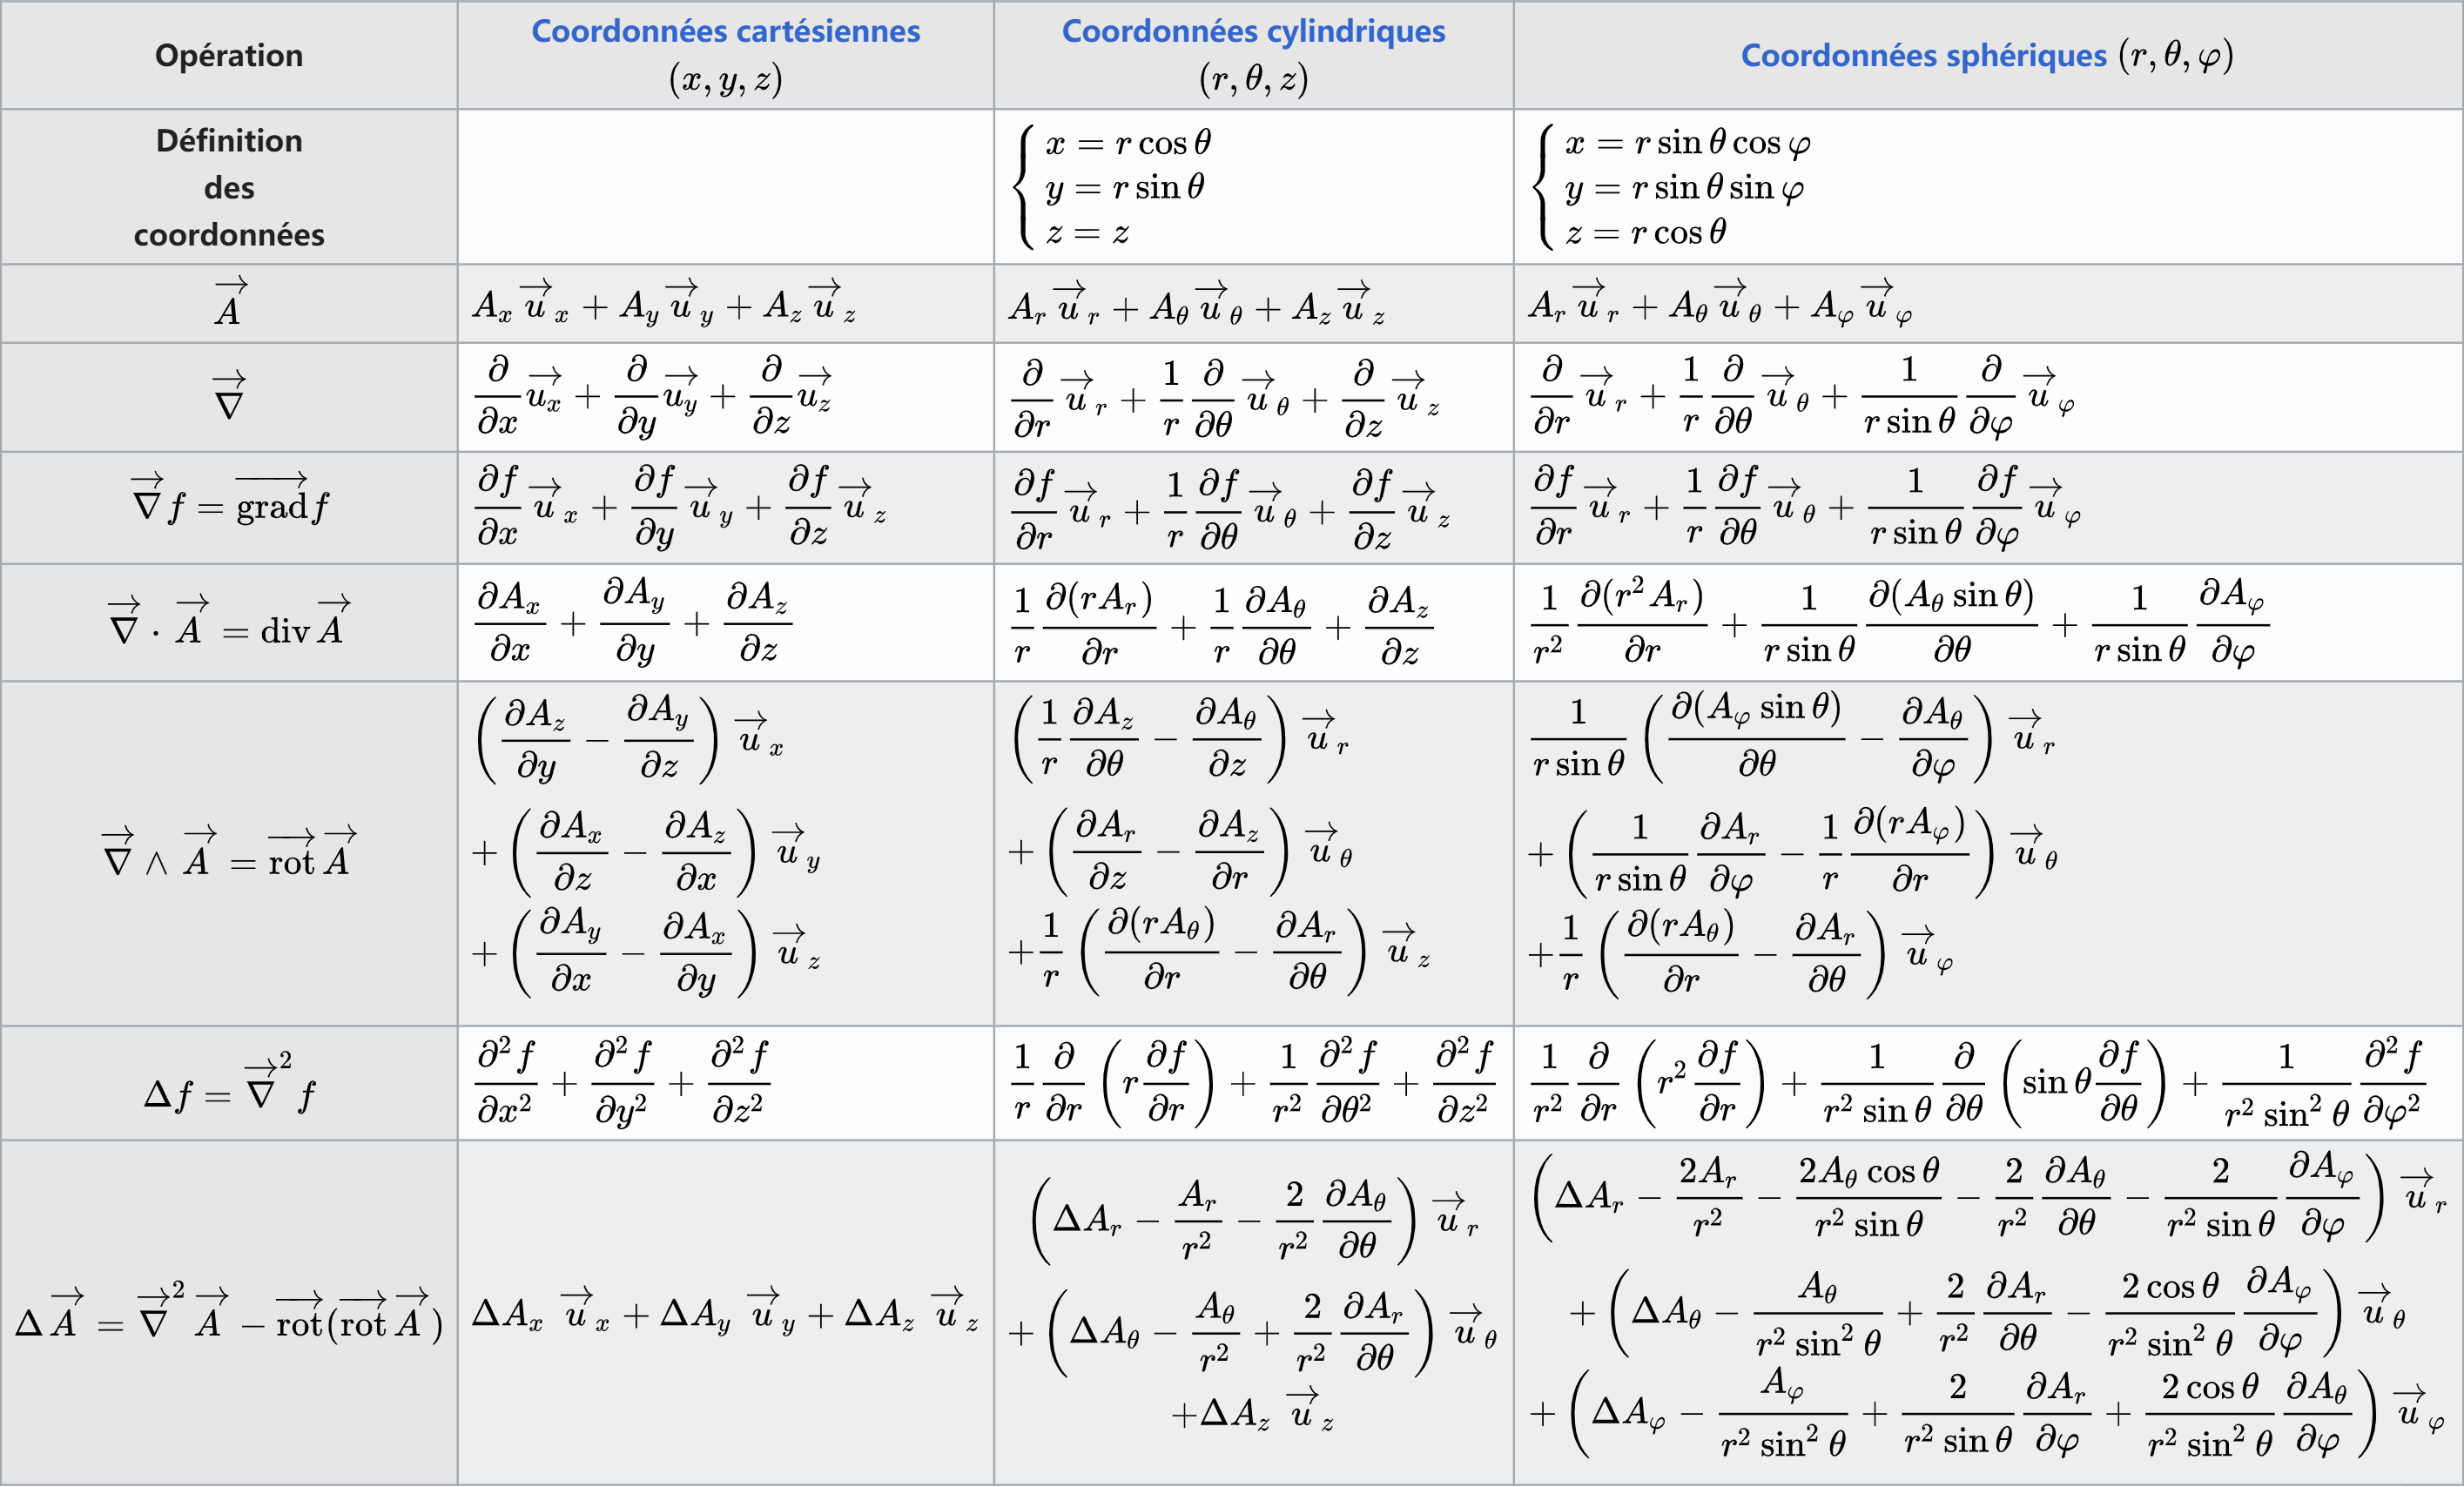
\includegraphics[scale=0.4]{nabla.png}
      \caption{$\nabla$算子(图源自法语wiki)}
      \label{fig:nabla}
    \end{figure}
  \subsection{Gauss散度定理 Théorème de flux-divergence}
    Gauss 散度定理,法语称 Théorème de flux-divergence 或者 Théorème de Green-Ostrogradski\footnote{在物理中偶尔会称Théorème de Gauss}.其说明矢量场穿过曲面的通量等于散度在曲面围起来的体积上的积分,即净流出量等于所有源点的和减去所有汇点的和.
    其在一维情况下等价于微积分基本定理,二维情况下等价于Green公式.
    $$
      \iiint \limits_{V} \text{div } \vec{F}\,dV=\oiint\limits_{\partial V}\vec{F} d\vec{S}  
    $$

\section{有限增长定理 Théorème des Accroissements Finis}
\subsection{Remarque: Rolle定理}
  设$\fai: I\subset \R\rightarrow \R$
  现在,我们将把Rolle定理推广.
\subsection{单实变函数的推广 Cas d'une variable réelle}
  设可微函数$f:I\subseteq \R\Rightarrow F$,其中$I$是开区间,$F$是实赋范向量空间.
  若有:
  $$
  \forall t\in I,\,\exists k>0,\, \left\lVert f'(t)\right\rVert _F\leq k 
  $$
  则有:
  $$
  \forall(x,y)\in I\times I,\,\left\lVert f(x)-f(y)\right\rVert _F\leq k\left\lvert x-y\right\rvert 
  $$
  \subsubsection{Démonstration}
  设$x<y$.考虑一个中间值$t\in[x,y]$.
  $$
  \forall \epsilon>0,\,\left\lVert f(x)-f(y)\right\rVert _F\leq (k+\epsilon)(t-x)+\epsilon
  $$
  通过证明以上的中间结论,加以$t$趋近于$y$即可证明推广公式.
  下面我们尝试证明这个中间结论.考虑集合:
  $$
  \mathcal{O}=\{t\in[x,y]\,|\,\left\lVert f(x)-f(y)\right\rVert _F> (k+\epsilon)(t-x)+\epsilon \}
  $$
  则$\mathcal{O}$是一个开集.下面要证明它是空集.
  利用反证法设其非空,则有下界$\underline{o}$.
  此下界$\underline{o}>x$且$\underline{o}\notin\mathcal{O}$,故有:
  $$
  \left\lVert f(\underline{o})-f(x)\right\rVert _F\leq (k+\epsilon)(\underline{o}-x)+\epsilon
  $$
  在$\underline{o}$附近,$  \exists \eta >0 ,\,\forall t\in(\underline{o},\underline{o}+\eta]$,有
  $$
    k\ge \left\lVert f'(\underline{o})\right\rVert _F\ge\frac{\left\lVert f(t)-f(\underline{o})\right\rVert _F}{\left\lvert t-\underline{o} \right\rvert} -\epsilon
  $$
  故有:
  $$
    \left\lVert f(t)-f(\underline{o})\right\rVert _F\leq (k+\epsilon)(t-\underline{o})
  $$
  可由三角不等式推出
  $$
    \left\lVert f(t)-f(\underline{o})\right\rVert _F\leq (k+\epsilon)(t-x)+\epsilon
  $$
  这说明$[\underline{o},\underline{o}+\eta]\cap\mathcal{O}=\varnothing$.
  又因为$t<y$,故对于一个足够小的$\eta$,仍有$\underline{o}+\eta<y $,
  即说明在$\underline{o} $与$\sup \mathcal{O}$中间存在至少一个$\underline{o}+\eta$,也即$\underline{o}\neq \sup \mathcal{O}$,与原假设矛盾.

\subsubsection{Proposition}
  设可微函数$f:I\subseteq \R\rightarrow F$,其中$I$是开区间,$F$是实Banach空间.
  若存在可导函数$\fai: I\rightarrow \R$使得:
  $$
  \forall t\in I,\,\exists k>0,\, \left\lVert f'(t)\right\rVert _F\leq \fai'(t)
  $$
  则有
  $$
  \forall(x,y)\in I\times I,\,\left\lVert f(x)-f(y)\right\rVert _F\leq \left\lvert \fai(x)-\fai(y)\right\rvert 
  $$
  \subsection{更一般的推广 Cas général}
  如上文所述,给出一般的赋范空间$E,F$上的可微函数函数$f:U\subseteq E\rightarrow F$.
  若有:
  $$
  \forall u\in U,\,\exists k>0,\,\normmm{\di f(u)}\leq k 
  $$
  则有:
  $$
  \forall(x,y)\in U\times U,\,\left\lVert f(x)-f(y)\right\rVert _F\leq k\left\lVert x-y\right\rVert _E
  $$
  \subsubsection{Démonstration}\noindent
  借助一个可导的辅助函数:
  $$
    g:[0,1]\rightarrow F
  $$
  $$
    t\mapsto f(x+t(y-x))
  $$
  其导数$g'(t)=\di f(x+t(y-x))(y-x)$满足:
  $$
  \forall t\in[0,1],\,\left\lVert g'(t)\right\rVert _F\leq k\left\lVert y-x\right\rVert _E
  $$
  根据单实变函数的结论,有:
  $$
  \left\lVert f(y)-f(x)\right\rVert _F=\left\lVert g(1)-g(0)\right\rVert _F\leq k\left\lVert x-y\right\rVert _E
  $$
  \subsubsection{Proposition}
  该不等式的另一种表述形式为:
  $$
  \left\lVert f(y)-f(x)\right\rVert _F\leq \sup_{t\in[0,1]}\normmm{\di f(x+t(y-x))}\left\lVert x-y\right\rVert _E
  $$
  \subsection{Proposition: sur les ouverts connexes}
    \subsubsection{Remarque: 连通子集 sous-ensemble connexe}
    考虑一个Banach空间的子空间拓扑,若除了空集和它本身之外没有既开又闭的子集,那么它就是连通的.\\
    \indent
    Un sous-ensemble d'un espace de Banach est connexe s'il n'admet pas de sous-ensemble à la fois ouvert et fermé autre que l'ensemble vide et lui-même.
    \subsubsection{Théorème}
    设连通集$U\subseteq E\rightarrow F$上的可微函数$f$,若有:
    $$
      \forall x\in U,\,\di f(x)\equiv 0
    $$
    则$f$是一个常值映射.
    \subsubsection{Démonstration}
    $\forall x\in U,\,\exists \text{ 开球}B(x,r)\subset U$.
    由有限增量定理知,$\di f=0$意味着$\forall y\in B(x,r),\,f(x)=f(y)$,故$f$在$x$附近是常值映射.
    接下来考虑逆映射$f\fuyi$.显然有$f\fuyi(\{f(x)\})\subset U\neq\varnothing$.
    又因为$\{f(x)\}$作为单点集是闭集,故$f\fuyi(\{f(x)\})$也是闭集.
    而我们前面任选的开球都是开集,因此$f\fuyi(\{f(x)\})$是$U$上非空的既开又闭的集合,只能是$U$本身.

 \subsection{Proposition: sur $\C^1$ }
  设一族有限个赋范空间$E_1,\dots,E_n$, $E=E_1\times \cdots \times E_n$
  上的可微函数:
  $$
    f:U\subseteq E \rightarrow
  $$
  $$
    x=(x_1,\dots,x_n)\mapsto f(x)
  $$
  $f$是连续可微函数当且仅当
  $$
  \forall i\in[\![1,n]\!],\,y_i\mapsto (x_1,\dots,x_{i-1},y_i,x_{i+1},\dots,x_n)
  $$
  在$y_i=x_i$处可微,且其微分对应了$U$上的一个$\mathcal{L}(E:F)$的函数.
\section{局部反演定理/反函数定理 Théorème d'Inversion Locale}
\subsection{微分同胚 Difféomorphisme}
  设$U$和$V$分别是实Banach空间$E$和$F$上的两个开集,若其上的函数$f:U\rightarrow V$满足:
  \begin{itemize}
    \item $f$是一个双射
    \item $f\in\mathcal{C}^1(U)$,即$f$是$U$上的一阶连续可微函数
    \item $f^{-1}\in\C^1(V)$,即$f$是$V$上的一阶连续可微函数
  \end{itemize}
  则称$f$是一个从$U$到$V$的微分同胚映射,简称微分同胚(Difféomorphisme).
  \subsubsection{Remarque}
  回顾\prettyref{myref:tongpei}同胚的概念.
  \subsubsection{Exemple}
  $(-\frac{\pi}{2},\frac{\pi}{2})$上的 $\sin,\,\cos$ 函数是微分同胚.
  \subsubsection{Exemple}
  $x\mapsto x^3$不是微分同胚.
  \subsubsection{Proposition}
  若$f:U\rightarrow V$是微分同胚,则$\forall x\in U,\,\di f(x)$是$E$到$F$上的同构.且有:
  $$
    \forall y\in V,\,\di f^{-1}(y)=(\di f(f^{-1}(y)))^{-1}
  $$
  \subsubsection{Démonstration}
  设$y=f(x),\,g=f^{-1}$,则有:
  $$
    g\circ f=\Id_U \text{            且             }f\circ g=\Id_V
  $$
  由复合函数的求导法则知:
  $$
  \forall x\in U,\,\di g(y)\circ \di f(x)=\Id_E\text{            且             }\di f(x)\circ \di g(y)=\Id_F
  $$
  \subsubsection{Proposition}
  若存在$E$到$F$的微分同胚,则两个空间是同构的.若其中一个是有限维的,则另一个空间也具有相同的维度.
  \subsubsection{Proposition}
  设$f:U\rightarrow V$,且$f\in\C^1$.对$a\in U$

  \subsection{Banach不动点定理 Théorème de Banach-Picard}
    设$C$是Banach空间$E$上的闭非空闭集,存在压缩映射 $h:C\rightarrow C$,即:
    $$
      \exists k\in(0,1),\,\forall (x_1,x_2)\in C^2,\,\left\lVert h(x_1)-h(x_2)\right\rVert _E\leq k\left\lVert x_1-x_2\right\rVert _E
    $$
    则$C$中有且仅有一个映射到自身的点,即:
    $$
      \exists! \,x\in C,\,h(x)=x
    $$
    \indent
    Si $C$ est un fermé non vide d'un espace de Banach $E$ et si $h:C\rightarrow C$ est contractante, 
    il existe un unique $x\in C$ tel que $h(x) = x$.
    \subsubsection{Démonstration}
    补全\prettyref{myref:yasuoyingshe} 的压缩映射再说


  \subsection{反函数定理 Théorème d'inversion globale}
  设$E$上非空开集$U$上的连续可微映射$f:U\subset E\rightarrow F,\,f\in \C^1$,
  则\f 是一个$U$到$f(U)$上的微分同胚当且仅当\f 是一个单射且其任意一点$U$上的微分都是从$E$到$F$的同构.\\
  \indent
  Soit $f : U \rightarrow F$ une application de classe $\C^1 $ avec $U$ un ouvert non vide. 
  C'est un difféomorphisme de $U$ sur $f (U)$ si et seulement si elle est injective et sa différentielle est en tout point de $U$ un isomorphisme de $E$ sur $F$.
  \subsubsection{Démonstration}

  \subsection{$\R^n$上的反函数 Cas de $\R^n$}
  设单射$f:U\subset \R^n\rightarrow \R^n,\,f\in\C^1$,\f 是一个微分同胚当且仅当其Jacobi矩阵在$U$上不为0(可逆).\\
  \indent
  Soit $U$ un ouvert de $\R^n$ et $f : U \rightarrow \R^n$ injective et de classe $\C^1 $.
  Alors\f est un difféomorphisme si et seulement si le déterminant de sa matrice jacobienne ne s'annule pas sur $U$.

\section{隐函数定理 Théorème des Fonctions Implicites}
\subsection{隐函数 Fonction implicite}
    对非线性方程$f(x,y)=0$,若可以将$y$表示为$x$的函数,即$y=\fai(x)$,则称方程隐含(implicitement)地定义了$y$,或称$y$是$x$的隐函数.
    \subsubsection{Exemple}
\subsection{隐函数定理}
  Banach空间上的隐函数定理是反函数定理的另一种表达方式,或者说二者是等价的.
  该定理的表示为:\\

  \indent
  设Banach空间$E,\,F,\,G$ 上的函数$f:U\subset E\times F\rightarrow G,\,f\in\C^1$.
  设存在$(a,b)\in U$ 使得$f(a,b)=0_G$,且关于$y$的偏微分$\di_2f(a,b)$是$F$到$G$上的同构,
  则存在$U$中关于$(a,b)$的邻域$U_{(a,b)}$和$E$中关于$a$的邻域$W_a$,以及函数
  $\fai:W_a\rightarrow F,\,\fai\in \C^1$使得:
  $$
    ((x,y)\in U_{(a,b)}\land f(x,y)=0_G)\Leftrightarrow y=\fai(x)
  $$
  \indent
  Soit $U$ un ouvert de $E\times F$ et $f:U\rightarrow G$ une fonction de classe $\C^1$.
  On suppose qu'il existe $(a, b) \in U$ tel que $f(a,b)=0_G$ et la différentielle partielle de $f$ par rapport à $y$, 
  $\di_2 f$ est telle que $\di_2 f (a, b)$ soit un isomorphisme de $F$ sur $G$.
  Alors il existe un voisinage ouvert $U(a,b)$ de $(a, b)$ dans $U$, 
  un voisinage ouvert $W_a$ de a dans $E$ et une fonction $\fai \in \C^1(W_a; F)$ telle que$((x,y)\in U_{(a,b)}\text{ et } f(x,y)=0_G)\Leftrightarrow y=\fai(x)$.
  \subsubsection{Démonstration}
  根据前面的局部反演定理,设函数:
  $$
    g:U\rightarrow E\times G
  $$
  $$
    (x,y)\mapsto (x,f(x,y))
  $$
  显然有$g\in\C^1 $且:
  $$
    \forall (x,y)\in U,\,\forall(h.k)\in E\times F,\,\di g(x,y)(h,k)=(h,\di_1f(x,y)\cdot h+\di_2f(x,y)\cdot k)
  $$
  其中$\di_1f$是$f$关于$x$的偏微分.
  接下来证明$\di g(a,b)$是$E\times F$到$E\times G$上的同构:
  \begin{align*}
    & \forall(h',k')\in E\times G:\,\\
    & (h,k)\in E\times F\land \di g(a,b)\cdot(h,k)=(h',k')\\
    & \Leftrightarrow h=h'\land k=(\di_2f(a,b))\fuyi(k'-\di_1f(a,b)\cdot h)
  \end{align*}
  因此$\di g(a,b)$是$E\times F$到$E\times G$上的同构.考虑其逆映射$(\di g(a,b))\fuyi$:
  $$
  (\di g(a,b))\fuyi:E\times G\rightarrow E\times F
  $$
  $$
    (h',k')\mapsto (h',(\di_2f(a,b))\fuyi(k'-\di_1f(a,b)\cdot h'))
  $$
  因此,$g$是$(a,b)$附近邻域$U_{(a,b)}$到$(a,0)$附近邻域上的一个微分同胚.
  设这个邻域是$W_a\times Z_0$,其中$W_a$是$a$的邻域,$Z_0$是$0_G$的邻域.
  则$g$的逆映射有以下形式:
  $$
    g\fuyi(x,z)=(x,\phi(x,z))
  $$
  其中$\phi$是$W_a\times Z_0$上的连续可微函数,也即:
  \begin{align*}
     ((x,y)\in U_{(a,b)}\land f(x,y)=z)
     \Leftrightarrow ((x,z)\in W_a\times Z_0\land y=\phi(x,z))
  \end{align*}
  特别地,有:
  $$
  ((x,y)\in U_{(a,b)}\land f(x,y)=0)\Leftrightarrow(x\in W_a\land y=\fai(x))
  $$
  \subsection{Proposition}
  尝试缩小$W_a$的范围,则有:
  $$
  \forall (x,h)\in W_a\times E,\,\di \fai(x)\cdot h=-(\di_2f(x,\fai(x)))\fuyi\di_1f(x,\fai(x))\cdot h
  $$
  \subsubsection{Démonstration}
  通过连续映射$\di_2f$将开集 $\text{Isom}(F:G)$的逆像包含在其中,且其包含了点$(a,b)$.
  设$\forall x\in W_a,\,\di_2f(x,\fai(x))\in\text{Isom}(F:G)$,映射$x\mapsto f(x,\fai(x))$的微分指出了其在$W_a$上的值都是0.










\section{二阶微分 Différentielle seconde}
\subsection{二次可微函数}
  考虑一个实Banach空间上的映射$f:U\subset E\rightarrow F$,若对于任意的$x\in U$,$f$在$x$处都是可微的,
  且其关于$x$邻域$U_x$上的微分$\di f:U_x\rightarrow \mathcal{L}(E;F)$在$x$处也是可微的,则称$f$在$U$上是二次可微的.\\
  \indent
  Une fontion f définie sur un ouvert non vide $U$ d'un \RR-espace de Banach $E$ et à valeurs dans un \RR-espace de Banach $F$ est dite 
  deux fois différentiable en $x \in U$ si elle est différentiable dans un voisinage ouvert $U_x$ de $x$ et si sa différentielle 
  $\di f:U_x\rightarrow \mathcal{L}(E;F)$ est différentiable en $x$.
  \subsubsection{Proposition}
  一些关于等距同构的内容,暂时略掉,没学明白.
\subsection{二阶微分}
  定义二阶微分(映射)为:
  $$
    \di^2f:U\rightarrow\mathcal{L}(E,E;F)
  $$
  $$
    x\mapsto \di^2f(x)
  $$
  $$
  \forall(h,k)\in E\times E,\,\di^2f(x)\cdot(h,k)=\di(\di f)(x)\cdot h\cdot k
  $$
  \subsubsection{Remarque}
  \subsubsection{Exemple}
  \begin{itemize}
    \item 仿射变换$f:x\mapsto \ell(x)+b$是二阶可微的,且$\di^2f(x)=0$
    \item 二次映射$f:x\mapsto \phi(x,x),\,\phi\in\mathcal{L}(E;F)$是二阶可微的,其二次微分是常数.
  \end{itemize}

\subsection{Schwarz微分定理 Théorème de Schwarz}
  若$f:U\subset E\rightarrow F$在$x\in U$处二次可微,则$\di^2f(x)$是一个对称双线性映射.\\
  \indent
  Si $f:U\subset E\rightarrow F$ deux fois différentiable en $x\in U$ alors $\di^2f(x)$ est une application bilinéaire symétrique.
  \subsubsection{Démonstration}
  该定理的证明需要一个引理:


  对函数$f:U\subset E\rightarrow F$和一点$x\in U$,考虑$(0,0)$周围的邻域上的函数
  $$
    A:(h,k)\mapsto f(x+h+k)-f(x+h)-f(x+k)+f(x)
  $$
  若\f 在$x$处二次可微,则有:
  $$
    \lim_{(h,k)\rightarrow(0,0)}\frac{A(h,k)-\di^2f(x)\cdot(h,k)}{\left\lVert h\right\rVert^2+\left\lVert k\right\rVert^2}=0
  $$
\subsection{在有限维空间上 En dimension finie}
  设有限维空间$E=\R^p$上的一组典范基$\mathcal{B}=(e_1,\cdots,e_p)$,若\f 是$U\subset \R^p$上的二次可微函数,有:
  $$
    \forall x\in U,\,\forall(i,j)\in[\![1,p]\!]^2,\, \di^2f(x)\cdot(e_i,e_j)=\frac{\pian}{\pian x_i}\frac{\pian f}{\pian x_j}(x)
  $$
  并且Schwarz定理表明$\di^2f(x)$是一个对称双线性映射,即:
  $$
    \frac{\pian}{\pian x_i}\frac{\pian f}{\pian x_j}(x)=\frac{\pian}{\pian x_j}\frac{\pian f}{\pian x_i}(x)=\frac{\pian^2f}{\pian x_i\pian x_j}(x)
  $$
  且对于$\R^p$中的向量$h$和$k$,有:
  $$
    \di^2f(x)\cdot(h,k)=\sum_{i=1}^p\sum_{j=1}^ph_ik_j\frac{\pian^2f}{\pian x_i\pian x_j}(x)
  $$
\subsection{Hess矩阵 Matrice Hessienne}
  在有限维空间上,二次微分可以用一个矩阵来表示,这个矩阵就是Hess矩阵.\\
  \indent
  设$E=\R^p$,则$f:U\subset \R^p\rightarrow \R$在$x\in U$处二次可微,则其Hess矩阵为:
  $$
    \Hess f(x)=\left(\frac{\pian^2f}{\pian x_i\pian x_j}(x)\right)_{(i,j)\in[\![1,p]\!]^2}
  $$
\subsection{Schwarz定理有限维推广}
  设$f:U\subset \R^p\rightarrow \R$在$x\in U$处二次可微,则其Hess矩阵是对称的.
  且对于$\R^p$中的向量$h$和$k$,有:
  $$
    \di^2f(x)\cdot(h,k)=\langle h,\text{Hess }f(x)k\rangle 
  $$
  其中$\langle \cdot,\cdot\rangle$是$\R^p$空间上的典范内积.
  \subsubsection{Remarque}
  \begin{itemize}
    \item 若$f:U\subset \R^3\rightarrow \R^3$在$x\in U$处二次可微,则$\text{div }\overrightarrow{\text{rot }} f=\nabla\cdot(\nabla\times f)=0$.
    \item 若$\fai:U\subset \R^3\rightarrow \R^3$在$x\in U$处二次可微,则$\overrightarrow{\text{rot }} \overrightarrow{\text{grad }} \fai=\nabla\cdot(\nabla f)=0$.
  \end{itemize}
\section{高阶微分 Différentielles d'Ordre Supérieur}
  \subsection{Définition}
  设实Banach空间上的映射$f:U\subset E\rightarrow F$,\n 是大于2的整数.
  若有\f 在$x\in U$的邻域$U_x$上可微,且其微分$\di f:U_x\rightarrow\mathcal{L}(E;F)$是$(n-1)$阶可微的,
  则称\f 在$x$处$n$阶可微.


  \indent
  Soit une fontion \f définie sur un ouvert (non vide) $U$ d'un \RR-espace de Banach $E$ et à valeurs dans un \RR-espace de Banach $F$, 
  et \n un entier au moins égal à 2. 
  On dit qu'elle est \n fois différentiable en $x \in U$ si elle est différentiable dans un voisinage ouvert $U_x$ de \x et
   si sa différentielle $\di f:U_x\rightarrow\mathcal{L}(E;F)$ est $(n-1)$ fois différentiable en \x.
  \subsubsection{Remarque}
  同理,若$\forall x\in U$, \f 在\x 处都是$n$阶可微的,则称\f 在$U$上是$n$阶可微的
  \subsubsection{Proposition}
  \begin{itemize}
    \item   $\di f\in\C^{n-1}$则有$ f\in\C^n$
    \item   $\forall n\ge 1,\,\di f\in\C^{n}$则有$f\in\C^\infty$
  \end{itemize}
  \subsection{\n 阶可微的传递性}
  设$f:U\subset E\rightarrow F$在$x\in U$上\n 阶可微,
  $g:V\subset F\rightarrow G$在$y=f(x)\in V$上\n 阶可微,
  则$g\circ f$在$x$上\n 阶可微,且有:
  $$
    \di^n(g\circ f)(x)=\di^n g(f(x))\circ\di^n f(x)
  $$
  若有$f\in\C^n,\,g\in\C^n$,则有$g\circ f\in\C^n$.
  \subsubsection{Démonstration}
  $n=1$易证可得,后用数学归纳法.
  \subsubsection{Proposition}
  若\f 是$U$到$V$上的微分同胚且$f\in\C^n$,则$f\fuyi\in\C^n$.
  \subsection{对称映射 Application Symétrique}
  设$E$和$F$是实Banach空间,$\mathcal{L}_n(E; F)$表示从$E^n$到$F$的连续$n$-线性映射的集合.
  对于任意的排列$\sigma$($\sigma$是集合$\{1,\dots, n\}$上的一个置换)以及任意的$n$元组$(x_1,\dots, x_n) \in E^n$,若有:
  $$
    \phi(x_{\sigma(1)},\dots, x_{\sigma(n)})=\phi(x_1,\dots, x_n)
  $$
  那么称映射$\phi \in \mathcal{L}_n(E; F)$为对称映射.其集合记为$\mathcal{L}_p^s(E; F) $


  \indent
  Soient $E$ et $F$ des \RR-espaces de Banach, et $\mathcal{L}_n(E; F)$ l'espace des applications \n-linéaires continues sur $E^n$. 
  Une application $\phi \in \mathcal{L}_n(E; F)$ est dite symétrique si pour toute permutation $\sigma$ de l'ensemble $\{1,\dots, n\}$ et pour tout \n-uplet $(x_1,\dots, x_n) \in E^n$:
  $$
    \phi(x_{\sigma(1)},\dots, x_{\sigma(n)})=\phi(x_1,\dots, x_n)
  $$
  Comme signalé en préambule, on notera $\mathcal{L}_p^s(E; F) $ l'espace des applications \n-linéaires continues et symétriques sur $E^n$.
  \subsubsection{Proposition}
  (待修改) 函数$f:U\subset E\rightarrow F$在$x\in U$上\n 阶可微,当且仅当:
  \begin{enumerate}
    \item 存在$U_x$使得函数
  $$
    \di^p f:U_x\rightarrow\mathcal{L}_p^s(E; F),\,p\leq n-1,\,\di^nf(x)\in\mathcal{L}_n^s(E; F)
  $$
    \item $\di^1f=\di f$
    \item $\forall p\leq n-2,\,\di^p f$在$U_x$上可微
    \item $\forall y\in U_x,\,\forall(h_1,\dots,h_{p+1})\in E^{p+1}$,有:
  $$
    \di^{p+1}f(y)(h_1,\dots,h_{p+1})=\di_{p+1}g^{[p]}(h_1,\dots,h_p,y)\cdot h_{p+1}
  $$
  其中:
  $$
    g^{[p]}(h_1,\dots,h_p,y)=\di^pf(y)(h_1,\dots,h_p)
  $$
\end{enumerate}
\section{高阶偏导数 Dérivées Partielles d'Ordre Supérieur}
  (需要修改)\\
    高阶偏导数本身没有什么理解上的困难.与之前一元函数的高阶导数内涵是一样的.
    但是在求解上,多了一个换序的问题,这也是本节主要研究的难点.
    首先请回顾\prettyref{myref:lagrangenote}里提到的偏导的表示方法.
    为了能更清晰地阐释内容,我们可能会混用这些符号,请时刻留意.\\

    考虑一个函数$f(x,y)$,其关于$x$的偏导$\frac{\partial f}{\partial x}=f_x(x,y)$,
    关于$y$的偏导$\frac{\partial f}{\partial x}=f_y(x,y)$.记:
    $$
    \frac{\partial f_x(x,y)}{\partial x}=\frac{\partial ^2f}{\partial x^2}=f_{xx}
    $$
    $$
    \frac{\partial f_y(x,y)}{\partial y}=\frac{\partial ^2f}{\partial y^2}=f_{yy}
    $$
    $$
    \frac{\partial f_x(x,y)}{\partial y}=\frac{\partial ^2f}{\partial y\partial x}=f_{xy}
    $$
    $$
    \frac{\partial f_y(x,y)}{\partial x}=\frac{\partial ^2f}{\partial x\partial y}=f_{yx}
    $$
    这里需要注意,当我们采用Leibniz符号时,分数线下面的求导次序是从右往左,与复合函数的映射顺序一致.
    $\frac{\partial ^2f}{\partial y\partial x} $是函数$f$先对$x$求偏导后的导函数再对$y$求.
    而Lagrange符号的顺序刚好相反,从左往右求偏导,表示为$f_{xy}$.即:
    $$
      \frac{\partial ^nf}{\partial x_n\cdots \partial x_1} = f_{x_1\cdots x_n}
    $$
  \subsection{偏导算子极限的换序}
  正如我们在函数列与函数项级数中广泛讨论的极限换序问题一样,
  当高阶偏导数涉及到多个自变量的极限时,我们自然而然就会提出是否可以对极限进行换序的问题,也即,什么样的函数满足:
  $$
    \frac{\partial ^2f}{\partial y\partial x} =\frac{\partial ^2f}{\partial x\partial y} 
  $$
  
  首先肯定不是所有二阶可微的函数都满足这个条件.我们可以举出反例:
  \subsubsection{Exemple}
  考虑$\R^2$上的标量值函数
  $$
    f(x,y)=
    \begin{cases}
      \frac{xy(x^2-y^2)}{x^2+y^2} &x^2+y^2\neq 0\\
      0 &x^2+y^2= 0
      \end{cases}
  $$
  则有$f_{xy}=\frac{\partial ^2f}{\partial y\partial x}=-1$,$f_{yx}=\frac{\partial ^2f}{\partial x\partial y}=1$ ,偏导算子不可交换.\\
  \subsubsection{偏导算子的极限}
  接下来让我们从定义出发研究一下这两个二阶偏导算子:
  $$
  \frac{\partial ^2}{\partial x\partial y}f=\frac{\partial }{\partial x}f_y=\lim_{h\rightarrow 0}\frac{f_y(x+h,y)-f_y(x,y)}{h}
  $$
  且对函数$f_y(x+h,y)$,有:
  $$
    f_y(x+h,y)=\lim_{k\rightarrow 0}\frac{f(x+h,y+k)-f(x+h,y)}{k}
  $$
  设函数
  $$
  \Phi(h,k)=\frac{f(x+h,y+k)-f(x+h,y)}{hk}-\frac{f(x,y+k)-f(x,y)}{hk}
  $$
  则二阶导可以转换成$h,k$的极限问题:
  $$
   \frac{\partial ^2}{\partial x\partial y}f=\lim_{h\rightarrow 0}\lim_{k\rightarrow 0}\Phi(h,k)
  $$
  $$
   \frac{\partial ^2}{\partial y\partial x}f=\lim_{k\rightarrow 0}\lim_{h\rightarrow 0}\Phi(h,k)
  $$
  \subsection{二元函数偏导换序}
  设函数$f:D\subseteq \R^2\rightarrow \R$,点$(x_0,y_0)$的某个邻域内若有
  \begin{itemize}
    \item $f_{xy}$存在且有极限
    \item $f_{yx}$存在且有极限
    \item $f(x,y)$二重极限存在
  \end{itemize}
  则有:
  $$
  \frac{\partial ^2}{\partial x\partial y}f(x_0,y_0)=\frac{\partial ^2}{\partial y\partial x}f(x_0,y_0)
  $$
  \subsubsection{Démonstration}
  我们已经把二元换序问题变成了极限交换问题.此时可用极限交换定理,也即两个累次极限都存在,重极限存在,则三个极限相等且可交换累次极限.
  \subsubsection{Remarque}
  需要说明,并不是所有累次极限存在的函数重极限就存在.例如:
  $$
  f(x,y)=
    \begin{cases}
      \frac{xy}{x^2+y^2} &x^2+y^2\neq 0\\
      0 &x^2+y^2= 0
      \end{cases}
  $$
  有
  $$
    \lim_{y\rightarrow 0}\lim_{x\rightarrow 0}f(x,y)=\lim_{x\rightarrow 0}\lim_{y\rightarrow 0}f(x,y)=0
  $$
  然而考虑沿直线$y=mx$方向趋近时,重极限
  $$
      \lim_{(x,y)\rightarrow(0,0)}f(x,y)=\lim_{x\rightarrow 0}\frac{mx^2}{x^2+m^2x^2}=\frac{m}{1+m^2}\neq 0
  $$
  \subsubsection{Remarque}
  同理,重极限和一个累次极限都存在,也不代表另一个累次极限就存在.例如:
  $$
  f(x,y)=
    \begin{cases}
      x+y\sin(\frac{1}{x}) &x\neq 0\\
      0 &x= 0
      \end{cases}
  $$
  有
  $$
  \lim_{x\rightarrow 0}\lim_{y\rightarrow 0}f(x,y)=\lim_{(x,y)\rightarrow(0,0)}f(x,y)=0\, (\text{利用}\left\lvert f(x,y)\right\rvert \leq\left\lvert x\right\rvert+\left\lvert y\right\rvert)
  $$
  \subsection{Proposition: 多元函数偏导换序}
  对多元函数的偏导,只需要将二元函数进行简单的推广即可.事实上,考虑高阶导数:
  $$
  \frac{\partial^kf}{\partial x_1,\cdots,\partial x_i,\cdots,\partial x_j,\cdots,\partial x_k}
  $$
  只需证明对于任意$x_i$和$x_j$的偏导是可换序的,则整体都是可换序的.不同的换序可以通过多个两两换序得到(这里不加以证明).
  

  
\section{高阶Taylor展开  Formules de Taylor}
\subsection{积分余项展开 Formule de Taylor avec reste intégral}
  \subsubsection{Remarque}
  设\RR 上的区间$I$和Banach空间$F$,函数:
  $$
    g:I\rightarrow F
  $$
  是$(n+1)$阶可导,记其$p$阶导数为$g^{(p)}$.则有:
  $$
    \forall t\in I,\,\frac{\di}{\di t}(g(t)+\sum_{p=1}^{man}\frac{(1-t)^p}{p!}g^{(p)}(t))=\frac{(1-t)^n}{n!}g^{(n+1)}(t)
  $$
  \subsubsection{Remarque}
  设$(a,b)\in\R^2,\,a\leq b$.Banach空间$F$.
  Riemann积分在区间$[a,b]$上定义了一个连续线性映射,作用于$\C([a,b];F)$.
  对任意的$g\in \C([a,b];F)$,其在$[a,b]$上的Riemann积分满足:
  $$
  \left\lVert \int_{a}^{b} g(t) \,\di t \right\rVert \leq \int_{a}^{b} \left\lVert g(t)\right\rVert  \,\di t\leq (b-a)\max_{t\in[a,b]}\left\lVert g(t)\right\rVert
  $$
  若$F$是有限维的,也即$\R^p$,则$\int_{a}^{b} g(t) \,\di t$是一个向量,其分量为$\int_{a}^{b} g_i(t) \,\di t$,其中$i$是典范基的分量.
  \subsubsection{Proposition}
  若\RR 上的开区间$I$包含$[0,1]$,$g:I\rightarrow F\in\C^{n+1}$,则有:
  $$
  g(1)-g(0)-\sum_{p=1}^{n}\frac{1}{p!}g^{(p)}(0)=
  \int_{0}^{1}\frac{(1-t)^n}{n!}g^{(n+1)}(t) \,\di t
  $$
  \subsubsection{Définition}
  对于任意的$h\in E$和$n \in\N^*$(自然数的非零元),我们用$h^{[n]}$表示由\n 个向量组成的元组,所有的向量都等于$h$.\\
  \indent
  Pour tout $h\in E$ et $n \in\N^*$, on désigne par $h^{[n]}$ le $n$-uplet vecteurs tous égaux à $h$.
  \subsubsection{Formule}
  设$E$,$F$是Banach空间,$U$是$E$的开集,$f:U\rightarrow F\in\C^{n+1}$,则对于任意的$x\in U$和$h\in E$使得$[x,x+h]\subseteq U$,有:
  $$
  f(x+h)-f(x)=\sum_{p=1}^{n}\frac{1}{p!}f^{(p)}(x)h^{[p]}+\int_{0}^{1}\frac{(1-t)^n}{n!}f^{(n+1)}(x+th)h^{[n+1]} \,\di t
  $$
  右边亦可写成;
  $$
  \sum_{p=1}^{n}\frac{1}{p!}\di^pf(x)\cdot h^{[p]}+\int_{0}^{1}\frac{(1-t)^n}{n!}\di^{n+1}f(x+th)\cdot h^{[n+1]} \,\di t
  $$
  \subsubsection{Exemple}
  \subsection{Lagrange余项展开 Formule de Taylor-Lagrange}
  \subsubsection{Proposition}
  若\RR 上的开区间$I$包含$[0,1]$,$g:I\rightarrow F$是${n+1}$阶可微函数,有:
  $$
  \forall t\in[0,1],\,\left\lVert g^{(n+1)}(t)\right\rVert \leq M
  $$
  则有:
  $$
  \left\lVert g(1)-g(0)-\sum_{p=1}^{n}\frac{1}{p!}g^{(p)}(0)\right\rVert \leq \frac{M}{(n+1)!}
  $$
  \subsubsection{Démonstration}
  设:
  $$
  f(t)=g(t)+\sum_{p=1}^{n}\frac{(1-t)^p}{p!}g^{(p)}(t)
  $$
  $$
  \fai(t)=-M\frac{(1-t)^{n+1}}{(n+1)!}
  $$
  则有
  $$
  \forall t\in[0,1],\,\left\lVert f'(t)\right\rVert \leq \fai'(t)
  $$
  \subsubsection{Formule}
  设$E$,$F$是Banach空间,$U$是$E$的开集,$f:U\rightarrow F$是${n+1}$阶可微函数,
  则对于任意的$x\in U$和$h\in E$使得$[x,x+h]\subseteq U$,若有:
  $$
  \max_{y\in[x,x+h]} \left\lVert \di^{n+1}f(y)\right\rVert _{\mathcal{L}_{n+1}(E;F)}\leq M
  $$
  则有:
  $$
  \left\lVert f(x+h)-f(x)-\sum_{p=1}^{n}\frac{1}{p!}\di^pf(x)\cdot h^{[p]}\right\rVert \leq \frac{M}{(n+1)!}\left\lVert h\right\rVert ^{n+1}
  $$
  \subsubsection{Démonstration}
  利用函数
  $$
  g(t)=f(x+th)
  $$
  \subsection{Formule de Taylor-Young}
  设$E$,$F$是Banach空间,$U$是$E$的开集,$f:U\rightarrow F$是$n$阶可微函数,
  则对于任意的$x\in U$和$h\in E$使得$[x,x+h]\subseteq U$,有:
  $$
  \left\lVert f(x+h)-f(x)-\sum_{p=1}^{n}\frac{1}{p!}\di^pf(x)\cdot h^{[p]}\right\rVert \leq 
  \mathcal{o}(\left\lVert h\right\rVert ^n)
  $$
  \subsubsection{Démonstration}

\section{极值 Extrema}
  \subsection{自由极值 Extrema Libres}
  设实Banach空间$E$,$U$是$E$的开集,$f$是定义在$U$上的实值函数.对一点$a\in U$:
  \subsubsection{极大值 minimum local}
  若存在a的邻域$V_a$使得$\forall x\in V_a,\,f(x)\leq a$,
  则称$a$是$f$的极大值点.
  \subsubsection{最大值 maximum globale}
  若$\forall x\in U,\,f(x)\leq a$,
  则称$a$是$f$在$U$的最大值点.
  若不等式严格成立,即$\forall x\in U,\,f(x)< a$,则称$a$是$f$在$U$的严格最大值点.
  \subsubsection{极小值 maximum local}
  若存在a的邻域$V_a$使得$\forall x\in V_a,\,f(x)\geq a$,
  则称$a$是$f$的极小值点.
  \subsubsection{最小值 minimum globale}
  若$\forall x\in U,\,f(x)\geq a$,
  则称$a$是$f$在$U$的最小值点.
  同理有严格最小值.
  \subsubsection{Remarque}
  回顾以下一元函数的极值情况:
  (略)
  \subsubsection{Proposition}
  设\f 是定义在实Banach空间$E$的开集$U$上的实值函数,且在$a\in U$处可微,则有:
  $$
  a\text{是}f\text{的极小值}\Rightarrow \di f(a)=0
  $$
  若\f 2阶可微,则有:
  $$
  \forall h\in E,\,\di^2f(a)\cdot h^{[2]}\geq 0
  $$
  反之,若对于$b\in U$,有 $\di f(b)=0$ 且 
  $\exists c>0,\,\forall h\in E,\,\di^2f(b)\cdot h^{[2]}\ge c\left\lVert h\right\rVert^2$,则$b$是\f 的极小值.
  \subsection{Lagrange乘数 Multiplicateurs de Lagrange}
  \subsubsection{相关极值 Extrema Liés}
  设\f 和 $g_1,\dots,g_p$ 是实Banach空间$E$上的开集$U$上的实值函数,
  对一点$a\in U$满足 $g_1(a)=\dots=g_p(a)=0$ ,若存在a的邻域$V_a$使得:
  $$
  \forall x\in V_a,\,g_1(x)=\dots=g_p(x)=0\Rightarrow f(x)\geq f(a)
  $$
  则称$a$是\f 在$U$上在约束$g_1=\dots=g_p=0$下的极大值点.\\
  \indent
  Si \f et $g_1,\dots,g_p$ sont des fonctions définies sur un ouvert $U$ d'un espace de Banach $E$ et à valeurs réelles, 
  un point $a\in U$ tel que $g_1(a)=\dots=g_p(a)=0$ est un minimum local de \f sous les contraintes $g_1=\dots=g_p=0$,
  s'il existe un voisinage $V_a$ de $a$ dans $U$ tel que:
  $$
  \forall x\in V_a,\,g_1(x)=\dots=g_p(x)=0\Rightarrow f(x)\geq f(a)
  $$
  \subsubsection{Proposition: Lagrange乘数}
  设\f 和 $g_1,\dots,g_p$ 是实Banach空间$E$上的开集$U$上的一阶连续可微实值函数($\C^1$),
  对一点$a\in U$满足 $g_1(a)=\dots=g_p(a)=0$,且其约束条件$g_1,\dots,g_p$是相互独立的.
  若$a$是约束条件$g_1,\dots,g_p$下的极小值,则有:
  $$
  \exists (\lambda_1,\dots,\lambda_p)\in\R^p,\,\di f(a)=\sum_{i=1}^{p}\lambda_i\di g_i(a)
  $$
  此时这组数$(\lambda_1,\dots,\lambda_p)$称为Lagrange乘数.
  \subsection{凸函数 Fonctions Convexes}
  \subsubsection{Définition}
  对实向量空间$E$上的子集$C$,若:
  $$
  \forall x,y\in C,\,\forall t\in[0,1],\,tx+(1-t)y\in C
  $$
  则称$C$是凸的(convexe).对凸集$C$上的实值函数$f$,若:
  $$
  \forall x,y\in C,\,\forall t\in[0,1],\,f(tx+(1-t)y)\leq tf(x)+(1-t)f(y)
  $$
  则称$f$是$C$上的凸函数(fonction convexe).
  若不等式严格成立,则称$f$是$C$上的严格凸函数.
  \subsubsection{Proposition}
  设$C$是实Banach空间上子集$U$的凸子集,$f:U\subset E\rightarrow \R$可微.
  则当且仅当:
  $$
    \forall(x,y)\in C^2,\,f(y)\geq f(x)+\di f(x)\cdot (y-x)
  $$
  \f 是$C$上的凸函数.
  \subsubsection{Proposition}
  设实Banach空间上的映射$f:U\rightarrow \R$,$C$是$U$的凸子集,有以下结论:
  \begin{enumerate}
    \item 若\f 是$C$上的凸函数,且有一个极小值,则该极小值也是$C$上的最小值.
    \item 若\f 是$C$上的严格凸函数,则其最多只有一个最小值,其也是严格最小值.
    \item 若\f 可微,则一点$a\in C$是最小值的必要条件是:$\forall y\in C,\,\di f(a)\cdot(y-a)\geq 0$
    \item 若\f 是$C$上的凸函数,则上一个结论的条件同时也是充分的.
  \end{enumerate}

  \subsubsection{凸函数的共轭函数 Fonction convexe conjugée}
  (需要多点内容)


  设\f 是$E$的子集$U$上的严格凸函数,$E^*$是$E$的对偶空间,其共轭函数$f^*$定义为:
  $$
      f^*:E^*\rightarrow (-\infty,+\infty]
  $$
  $$
      y\mapsto \sup_{x\in U}\left\{\di f(x)\cdot y-f(x)\right\}
  $$
  这种对函数进行的共轭变换亦被称为Fenchel-Moreau变换.
  共轭函数在优化方面有重要应用,在许多应用方法中,要求其取值是有界的,即$f^*:E^*\rightarrow \R$.

  \subsection{变分法简介 Introduction au calcul des variations}
  好难好难好难好难好难\\
  考虑函数空间$E=\C^1([0,1];\R)$上的范数:
  $$
  \left\lVert u\right\rVert _\infty=\max_{t\in[0,1]}\left\lvert u(t)\right\rvert _{\R^n}
  $$
  $$
    \left\lVert u\right\rVert =\max{\left\lVert u\right\rVert _\infty,\left\lVert u'\right\rVert _\infty}
  $$
  其中$u'$是$u$的导数.


  设$\R^n$上的两个点$a,b$,考虑凸集合$C=\{u(0)=a,u(1)=b\,|\,u\in E\}$和映射:
  $$
  \mathcal{A}:u\mapsto \int_0^1 L(u(t),u'(t)) \di t
  $$
  其中$L\in\C^2(\R^n\times \R^n;\R)$被称为Lagrange量(Lagrangien),$\mathcal{A}$是其相关的作用泛函(fonctionnelle d'action).
  显然$\mathcal{A}$在$E$上可微,故在$C$上有最小值$u$.
  则有$\forall h\in C-u,\, \di \mathcal{A}(u)\cdot h\geq 0$,也即$\forall h\in E,\,h(0)=h(1)=0$.
  这就将不等式变成了等式,即$u$是$\mathcal{A}$在$C$上的最小值的必要条件是,$\forall h\in E$使得$h(0)=h(1)=0$,有:
  $$
  \int_0^1 \sum_{i=1}^{n} \frac{\pian L}{\pian q_i}(u(t),u'(t)h_i(t))\di t+
  \int_0^1 \sum_{i=1}^{n} \frac{\pian L}{\pian q_i'}(u(t),u'(t)h_i'(t))\di t=0
  $$
  其中$q_i,q_i'$都是$L$的参数分量(les composantes des arguments de $L$).
  在变分法和拉格朗日力学中,$q_i,q_i'$.
  在物理应用中,我们考虑描述系统运动的函数,通常称为Lagrangian函数或Lagrangian密度($L$),
  这个函数取决于一组自变量,这些自变量通常表示系统的广义坐标和广义速度.
  

  如果$u\in\C^2$,我们可以简化为:
  $$
    \int_0^1 \sum_{i=1}^{n} (\frac{\pian L}{\pian q_i}(u(t),u'(t))-\frac{\di }{\di t}
    (\frac{\pian L}{\pian q_i'}(u(t),u'(t))))h_i(t)\di t=0
  $$
  若要使其对于任意的函数$h$都成立,则有以下充要条件:
  $$
    \forall t\in[0,1],\,\frac{\pian L}{\pian q_i}(u(t),u'(t))-\frac{\di }{\di t}
    (\frac{\pian L}{\pian q_i'}(u(t),u'(t)))=0
  $$
  也即$u$是以下微分方程的解:
  $$
  \forall t\in[0,1],\,\frac{\di}{\di t}( \frac{\pian L}{\pian q_i'}(u(t),u'(t)))=\frac{\pian L}{\pian q_i}(u(t),u'(t))
  $$
  该方程称为与函数$L$相关的Euler-Lagrange方程.可以简写为:
  $$
    \delta \mathcal{A}(u)=0
  $$
  其中$\delta \mathcal{A} $被称为$\mathcal{A}$的变分梯度(gradient variationnel),其定义为:
  $$
    \delta \mathcal{A}: \C^2([0,1];\R^n)\rightarrow \C^0([0,1];\R^n)
  $$
  $$
    u\mapsto \delta \mathcal{A}(u)
  $$
  $$
    \delta \mathcal{A}(u)_i(t)=\frac{\pian L}{\pian q_i}(u(t),u'(t))-\frac{\di }{\di t}
    (\frac{\pian L}{\pian q_i'}(u(t),u'(t)))
  $$
  若$L$是凸函数,则$\mathcal{A}$也是凸的,故其解$u$是最小值.
  若$L$不是凸函数,则其Euler-Lagrange方程不足以最小化$\mathcal{A}$.
  通过研究$\mathcal{A}$的Hessian矩阵,我们可以得到更多的信息.
  \subsubsection{Proposition}
  对泛函:
  $$
  \mathcal{A}:u\in\C^2([0,1];\R^n)\mapsto \int_0^1 L(u(t),u'(t)) \di t
  $$
  其中$L\in \C^2(\R^n\times\R^n;\R)$.
  有$\forall u\in\C^2([0,1];\R^n),\,\forall h\in  \C^2([0,1];\R^n)$使得
  $h(1)=h(0)=0\land h'(1)=h'(0)=0$,有:
  $$
  \frac{\di}{\di\theta}\mathcal{A}(u+\theta h)|_{\theta=0}=\langle \delta\mathcal{A}(u),h \rangle 
  $$
  $$
  \frac{\di^2}{\di\theta^2}\mathcal{A}(u+\theta h)|_{\theta=0}=\langle h,\Hess\mathcal{A}(u)h \rangle 
  $$
  其中:
  $$
  \langle u,v \rangle =\int_0^1 \sum_{i=1}^{n}u_i(t)v_i(t) \di t
  $$
  对于算子$\Hess\mathcal{A}(u)$,其定义为:
  $$
  \Hess\mathcal{A}(u)=-\frac{\di}{\di t}A(u)\frac{\di}{\di t}+B(u)\frac{\di}{\di t}+C(u)
  $$
  其中:
  $$
  A(u)_{i,j}= \frac{\pian^2 L}{\pian q_i'\pian q_j'}(u(t),u'(t))
  $$
  $$
  B(u)_{i,j}=2\frac{\pian^2 L}{\pian q_i\pian q_j'}(u(t),u'(t))
  %有问题,为什么不是\pian q_i\pian q_j'+\pian q_i'\pian q_j?
  $$
  $$
  C(u)_{i,j}=\frac{\pian^2 L}{\pian q_i\pian q_j}(u(t),u'(t))
  $$
  在集合$C=\{u(0)=a,u(1)=b,u'(0)=0,u'(1)=1\}$中,$u$是$\mathcal{A}$极小值的必要条件为:
  $$
  \delta\mathcal{A}(u)=0\land \forall h\in C,\,\langle h,\Hess\mathcal{A}(u)h \rangle \geq 0
  $$

  \section{微分形式 Formes différentielles}
  本开始的内容都很难,我大概率会在再学一遍之后重写.
  因此这几节都会相对简单.
  \subsection{矢量场和1-形式微分 Champs de vecteurs et 1-formes différentielles}
  \subsubsection{Définition}
  在$\R^n$中开集上的矢量场是一个从$\R^n$到$\R^n$的$\C^k$的函数,
  1-形式为分是从$\R^n$到线性空间$\mathcal{L}(\R^n;\R)$(又称为Pfaff形式).\\
  \indent
  Un champ de vecteurs (de classe $\C^k$ ) sur un ouvert de $\R^n$ est une application (de classe $\C^k$ ) à valeurs dans l'espace vectoriel $\R^n$. 
  Une 1-forme différentielle (de classe $\C^k$ ) sur un ouvert de $\R^n$ est une application (de classe $\C^k$ ) à valeurs dans l'espace vectoriel $L(\R^n; \R)$ des formes linéaires sur $\R^n$. 
  Les 1-formes différentielles sont aussi appelées formes de Pfaff.
  \subsubsection{Exemple}
  $V(x,y)=(\alpha x,\beta y)$是一个矢量场,$\theta(x,y)=alpha x+\beta y$是一个微分形式.
  \subsubsection{Remarque}
  \subsubsection{恰当的1-形式}
  对1-形式微分$\omega$,若存在可微函数\f 使得其全微分$\di f=\omega$,则称该1-形式微分是恰当的(exact).
  
  \subsection{高阶微分形式 Formes différentielles d'ordre supérieur}
  \subsubsection{Définition}
  作为对1-形式的扩展,我们可以定义$q$-形式,其中$q\in\N$.
  记 $\mathcal{A}_q(\R^n)$ 为 $\mathcal{L}_q (\R^n)$ 中的$q$-线性交替形式的向量子空间,即 $\phi \in\mathcal{L}_q (\R^n)$ 满足:
  $$
  \forall (u_1,\dots,u_q)\in\R^n,\text{其中有两个以上的向量相等}\,\phi(u_1,\dots,u_q)=0
  $$
  该过程体现的是$\phi$的反对称性,即有:
  $$
  \phi(u_1,\dots,u_j,\dots,u_i,\dots,u_q)=-\phi(u_1,\dots,u_i,\dots,u_j,\dots,u_q)
  $$
  \subsubsection{Proposition}
  设整数$q\geq 2$,对空间$\mathcal{A}_q(\R6^n)$,若$q>n$,则$\mathcal{A}_q(\R^n)=\{0\}$.
  反之,若$q\leq n$,则$\mathcal{A}_q(\R^n)$的维数为:
  $$
  \dim\mathcal{A}_q(\R^n)=\binom{n}{q}=\frac{n!}{q!(n-q)!}
  $$
  其由以下类型的线性$q$-形式产生:
  $$
  \di x_{i_1}\wedge\dots\wedge\di x_{i_q},\,1\leq i_1<\dots<i_q\leq n
  $$
  其中外积$\wedge$表示交替线性$q$-形式(q-forme linéaire alternée),定义为:
  $$
  (\di x_{i_1}\wedge\dots\wedge\di x_{i_q})(\frac{\pian }{\pian x_{j_1}},\dots,\frac{\pian }{\pian x_{j_q}})=
  \begin{cases}
    1&\forall k\in[\![1,q]\!],\,i_k=j_k,\\
    0&\{i_1,\dots,i_q\}\neq\{j_1,\dots,j_q\}.
  \end{cases}
  $$
  \subsubsection{Définition}
  对于给定的整数$q \geq 2$, $q$阶微分形式是一个定义在$\mathbb{R}^n$的开集上,取值于$q$阶线性交替形式空间$\mathcal{A}_q(\mathbb{R}^n)$的$\mathcal{C}^k$类映射.\\
  \indent
  Soit $q$ un entier supérieur ou égal à 2. 
  Une $q$-forme différentielle de classe $\C^k$ sur un ouvert de $\R^n$ est une application de classe $\C^k$ à valeurs dans l'espace vectoriel $\mathcal{A}_q(\R^n)$ des $q$-formes linéaires alternées sur $\R^n$. 
  (Les $q$-formes différentielles sont également appelées formes différentielles de degré $q$.)
  \subsubsection{Remarque}
  已知任意一个$q$阶微分形式$a$可以分解为:
  $$a = \sum\limits_{1\leq i_1<\ldots<i_q\leq n} a_{i_1,\ldots,i_q} dx_{i_1} \wedge \ldots \wedge dx_{i_q}$$
  其中$a_{i_1,\ldots,i_q}$是实值函数.
  反过来,如果对于$1 \leq i_1 < \ldots < i_q \leq n$,有$ai_1,\ldots,i_q \in \mathcal{C}^k(U; \mathbb{R})$,
  那么映射$x \mapsto \sum\limits_{1\leq i_1<\ldots<i_q\leq n} a_{i_1,\ldots,i_q}(x) dx_{i_1} \wedge \ldots \wedge dx_{i_q}$定义了一个$q$阶微分形式.


  为了与1-形式的定义保持一致,我们将$\mathcal{A}_1(\mathbb{R}^n)$也表示为线性形式空间$L(\mathbb{R}^n; \mathbb{R})$,并且按照约定,$\mathcal{A}_0(\mathbb{R}^n)$表示常函数空间.
  因此关于$q$阶微分形式的定义实际上适用于任意自然数$q$.0阶微分形式实际上就是一个实值函数.
  \subsection{外积 Produit extérieur}
  \subsubsection{Définition}
  首先考虑$\di x_1\wedge\dots\wedge\di x_q $的定义,其映射:
  $$
  \mathcal{L}(\R^n;\R)^q\to \mathcal{A}_1(\R^n)
  $$
  $$
  (\ell_1,\dots,\ell_q)\mapsto\ell_1\wedge\dots\wedge\ell_q
  $$
  本身就是一个$q-$线性交替形式,因此,
  对于任意给定的整数q和r,我们可以定义外积操作$\wedge$,将两个$q$-形式和$r$-形式的函数映射到一个($q+r$)-形式的函数空间中,即:
  $$
  \wedge:\mathcal{A}_q(\R^n)\times\mathcal{A}_r(\R^n)\to\mathcal{A}_{q+r}(\R^n)
  $$
  $$
  (\alpha,\beta)\mapsto\alpha\wedge\beta
  $$
  其中,对于:
  $$
  \alpha=\sum\limits_{1\leq i_1<\ldots<i_q\leq n}a_{i_1,\ldots,i_q}\di x_{i_1}\wedge\ldots\wedge\di x_{i_q}
  $$
  $$
  \beta=\sum\limits_{1\leq j_1<\ldots<j_r\leq n}b_{j_1,\ldots,j_r}\di x_{j_1}\wedge\ldots\wedge\di x_{j_r}
  $$
  其外积为:
  $$
  \alpha\wedge\beta=\sum\limits_{\substack{1\leq i_1<\ldots<i_q\leq n\\1\leq j_1<\ldots<j_r\leq n}}a_{i_1,\ldots,i_q}b_{j_1,\ldots,j_r}\di x_{i_1}\wedge\ldots\wedge\di x_{i_q}\wedge\di x_{j_1}\wedge\ldots\wedge\di x_{j_r}
  $$
  \subsubsection{Remarque}
  \begin{itemize}
    \item 外积是双线性的:对于任意的常数$k_1$和$k_2$,以及$a_1, a_2 \in \mathcal{A}_q(R^n)$和$b_1, b_2 \in \mathcal{A}_r(R^n)$,有
  \begin{align*}
  (k_1a_1 + k_2a_2) \wedge (k_1b_1 + k_2b_2) &= k_1k_1(a_1 \wedge b_1) + k_1k_2(a_1 \wedge b_2) \\
  &\quad+ k_2k_1(a_2 \wedge b_1) + k_2k_2(a_2 \wedge b_2)
  \end{align*}

  \item 外积满足结合律:对于任意的$a \in \mathcal{A}_q(R^n)$,$b \in \mathcal{A}_r(R^n)$和$c \in \mathcal{A}_s(R^n)$,有
  \[(a \wedge b) \wedge c = a \wedge (b \wedge c)\]

  \item 外积满足分配律:对于任意的$a_1, a_2 \in A^q(R^n)$和$b \in A^r(R^n)$,以及$c_1, c_2 \in A^q(R^n)$和$d \in A^r(R^n)$,有
  \[(a_1 + a_2) \wedge b = (a_1 \wedge b) + (a_2 \wedge b),\]
  \[a \wedge (b + c) = (a \wedge b) + (a \wedge c)\]

  \item 外积满足反交换律:对于任意的$a \in A^q(R^n)$和$b \in A^r(R^n)$,有
  \[a \wedge b = (-1)^{qr} b \wedge a,\]
  其中$(-1)^{qr}$表示$(-1)$的幂次方,$qr$为整数$q$和$r$的乘积的奇偶性.
  \end{itemize}
  \subsection{拉回 Tiré en arrière / Pullback}
  注意,拉回的法语名称是 tiré en arrière ,简称为 tirette ,但是在大量参考文献里,法国人都在用英语 pullback 表示拉回,称之为"le pullback".
  这似乎是因为在数学领域里面,"pullback"一词被广泛使用,并在国际数学界具有较高的认可度.
  因此,为了与国际数学习惯保持一致,法国人倾向于使用"le pullback"这个术语.
  但在阅读法语资料的时候,tiré en arrière, tirette 和 pullback都被用于表示拉回.
  另外值得一提的是,尽管完全看不出是个名词, tiré en arrière 是阳性名词,
  但其理论上对应的表示拉的名词 tire 是阴性名词,而 tirette 也是阴性名词.当然,pullback 又是阳性名词.
  \subsubsection{Définition}
  对一个0-形式微分,其可以通过变量的转换进行传递,即设$\R^n$上两个开集间的$\C^k$映射$\fai:V\to U$,对任意$\C^k$的0-形式微分$f:U\to\R$,
  其复合$f\circ \fai:V\to\R \in\C^k$.为了表示这种复合映射,定义$\fai^*f$:
  $$
  \fai^*f=f\circ\fai:V\to\R
  $$
  $$
  y\mapsto (\fai^*f)(y)=f(\fai(y))
  $$
  这里的$\fai^*:f\mapsto \fai^*f$变换就是0-形式微分的拉回.推广至任意阶的微分形式,有如下定义:
  \subsubsection{Définition}
  对于非零自然数q,设$\R^n$上两个开集间的$\C^{k+1}$映射$\fai:V\to U$,对于$U$上的q-形式微分$\alpha\in\C^k$,
  其通过$\fai$的拉回是$V$上的q-形式微分$\beta=\fai^*\alpha$:
  $$
  \beta(y)\cdot(v_1,\cdots,v_q)=\alpha(x)\cdot(u_1,\cdots,u_q)
  $$
  其中$x=\fai(y)$,且$u_k=\di \fai(y)\cdot v_k,\,k\in[\![1,q]\!]$.\\
  \indent
  Soit $q$ un entier naturel non nul. Soit $\fai:V\to U$ une fonction de classe $\C^{k+1}$ d'un ouvert $V$ de $\R^n$ sur un ouvert $U$.
  Le pullback par $\fai$ d'une q-forme différentielle $\alpha$ de classe $\C^k$ sur $U$ est $\beta=\fai^*\alpha$ la q-forme différentielle de classe $\C^k$ sur $V$ définie par 
  $\beta(y)(v_1,\cdots,v_q)=\alpha(x)\cdot(u_1,\cdots,u_q)$, où $x=\fai(y)$ et $u_k=\di \fai(y)\cdot v_k,\,k\in[\![1,q]\!]$.
  \subsubsection{Exemple}
  \begin{itemize}
    \item 对1-形式微分 $\alpha=\sum_{n}^{j=1}\alpha_j\di x_j$,其拉回为:
          $$
          \fai^*\alpha=\sum_{j=1}^{n}\sum_{i=1}^{n}(\alpha_i\circ \fai)\frac{\pian \fai_i}{\pian y_j}\di y_j=\sum_{i=1}^{n}(\alpha_i\circ \fai)\di\fai_i
          $$
    \item 对$n$-体积形式(forme volume)$\alpha=f\di x_1\wedge\cdot\wedge\di x_n$,其拉回为:
          $$
          \fai^*\alpha=(f\circ\fai)(\det\di\fai)\di y_1\wedge\cdot\wedge\di y_n
          $$
          其中$\det\di\fai$为$\fai$的Jacobi行列式.
    \item 对$n-1$-曲面形式(forme surfacique):
          $$
          \alpha=\sum_{i=1}^{n}f_idi x_1\wedge\cdot\wedge\di x_{i-1}\wedge\di x_{i+1}\wedge\cdot\wedge\di x_n
          $$
          其拉回为:
          $$
          \fai^*\alpha=\sum_{i=1}^{n}(f_i\circ\fai)(\text{cofact }\di\fai)_{i,j}\di y_1\wedge\cdot\wedge\di y_{i-1}\wedge\di y_{i+1}\wedge\cdot\wedge\di y_n
          $$
          其中$(\text{cofact }\di\fai)_{i,j}$为Jacobi矩阵在$(i,j)$处的余子式.
  \end{itemize}
  \subsubsection{纯形式 Forme pure}
  一个"纯(pure)"的形式指的是只包含单一次数的微分形式.
  例如,一个纯1-形式只包含一个单独的微分项,如$f \di x$,而不包含 $\di x \wedge \di y$ 或其他多项式.
  类似地,一个纯$q$-形式是一个$q$阶的微分形式,其中每个微分项都包含相同数量的微分项 $\di x_i$,并且没有包含 $\di x_i \wedge \di x_j$ 或其他更高阶的项.
  \subsubsection{Proposition}
  对一个纯的$q$-形式$\alpha=f\di x_{i_1}\wedge\cdot\wedge\di x_{i_q}$,有:
  $$
  \fai^*\alpha=(f\circ\fai)\di\fai_{i_1}\wedge\cdot\wedge\di\fai_{i_q}
  $$
  对任意纯的$q$-形式$\alpha$和$r$-形式$\beta$,有:
  $$
  \fai^*(\alpha\wedge\beta)=\fai^*\alpha\wedge\fai^*\beta
  $$
  \subsubsection{Démonstration}
  略.
  \subsection{外微分 Différentielle extérieure}
  \subsubsection{Définition}
  对一个$\C^k$类的$q$-形式
  $$
  \alpha=\sum_{1\leq i_1<\cdots<i_q\leq n}\alpha_{i_1,\cdots,i_q}\di x_{i_1}\wedge\cdots\wedge\di x_{i_q}
  $$
  其外微分为一个$\C^{k-1}$类的$q+1$-形式:
  $$
  \die \alpha=\sum_{i=1}^{n}\sum_{1\leq i_1<\cdots<i_q\leq n}\frac{\pian \alpha_{i_1,\dots,i_q}}{\pian x_i}\di x_i
  $$
  且认为对于0-形式的外微分与其在函数意义下的微分相等:
  $$
  \die f=\di f=\sum_{i=1}^{n}\frac{\pian f}{\pian x_i}\di x_i
  $$
  \subsubsection{Proposition}\label{myref:exact_est_ferme}
  对任意$k\geq 2$,$\C^k$类的微分形式$\alpha$都有:
  $$
  \die(\die\alpha)=0
  $$
  \subsubsection{Démonstration}
  对$ \alpha=\sum_{1\leq i_1<\cdots<i_q\leq n}\alpha_{i_1,\cdots,i_q}\di x_{i_1}\wedge\cdots\wedge\di x_{i_q}$,有:
  $$
    \die(\die\alpha)=\sum_{1\leq i_1<\cdots<i_q\leq n}( \sum_{j=1}^{n}\sum_{i=1}^{n}\frac{\pian^2\alpha_{i_1,\cdots,i_q}}{\pian x_j\pian x_i}\di x_j\wedge\di x_i )\wedge\di x_{i_1}\wedge\cdots\wedge\di x_{i_q}
  $$
  由外积的反对称性$\di x_j\wedge\di x_i=-\di x_j\wedge\di x_j$和Schwarz定理,对二阶可微\f,有:
  $$
  \sum_{j=1}^{n}\sum_{i=1}^{n}\frac{\pian^2f}{\pian x_j\pian x_i}=0
  $$
  \subsubsection{Définition}
  对微分形式$\alpha$,若存在微分形式$\beta$使得$\die\beta=\alpha$,则称$\alpha$是恰当形式.
  若$\die \alpha=0$,则称$\alpha$是闭形式(forme fermée).\\
  \indent
  Une forme différentielle $\alpha$ est dite exacte s'il existe une forme différentielle $\beta$ telle que $\die \beta=\alpha$.
  Une forme différentielle $\alpha$ est dite fermée si $\die \alpha=0$.
  \subsubsection{Remarque}
  对$q\geq 1$,不要混淆其外微分和$U$到$\mathcal{A}_q(\R^n)$上映射的微分混淆.
  例如$q=1$时,对$\alpha=\sum_{j=1}^{n}\alpha_j\di x_j$,有:
  $$
  \die \alpha=\sum_{1\leq i< j\leq n}(\frac{\pian \alpha_j}{\pian x_i}-\frac{\pian\alpha_j}{\pian x_i})\di x_i\wedge\di x_j
  $$
  也即$\forall h\in\R^n,k\in\R^n$,有:
  $$
  \die \alpha(h,k)=\sum_{1\leq i< j\leq n}(\frac{\pian \alpha_j}{\pian x_i}-\frac{\pian\alpha_j}{\pian x_i})(h_ik_j-h_jk_i)
  $$
  而对于$U$到$\mathcal{A}_1(\R^n)$上的映射$\alpha$,有:
  $$
  \di\alpha(x)\cdots h=\sum_{i,j=1}^{n}\frac{\pian\alpha_j}{\pian x_i}h_i\di x_j
  $$
  则有仅当映射$(h,k)\mapsto(\di\alpha(x)\cdots h)\cdots k$是对称的时,$\die \alpha=0$.
  \section{Poincaré定理 Théorème de Poincaré}
  \prettyref{myref:exact_est_ferme}告诉我们,每个恰当微分形式都是闭的,但其逆命题并不一定成立.
  这取决于开集$U$的拓扑性质.本节我们简单介绍Poincaré定理.

  \subsection{单连通 Simplement connexe}
  \subsubsection{Définition}
  称$\mathbb{R}^n$ 中的开集 $U$ 是单连通的,或者是1-连通的,如果对于任意的简单闭曲线(或回路),即没有重复点的曲线,满足:
  $$
  \{\theta(t)\,|\,t\in[0,1] \}
  $$
  其中 $\theta:[0,1]\to U$ 是连续的、在 $(0,1)$ 上是单射且满足 $\theta(0)=\theta(1)$,那么存在一个点 $x_0\in U$ 和一个连续的同伦映射 $\Theta :[0,1]\times[0,1]\to U$,满足:
  $$
  \Theta (\cdot,0)\equiv x_0\, \land\, \Theta (\cdot,1)\equiv \theta
  $$
  \indent
  Un ouvert $U$ de $\R^n$ est dit simplement connexe, ou encore 1-connexe si, 
  pour tout courbe fermée (ou lacet) simple, c'est-à-dire sans point double, on a:
  $$
  \{\theta(t)\,|\,t\in[0,1] \}
  $$
  avec $\theta:[0,1]\to U$ continue, injective sur $(0,1)$ et telle $\theta(0)=\theta(1)$, il existe un point $x_0\in U$ 
  et une application homotopie $\Theta :[0,1]\times[0,1]\to U$ continue telle que:
  $$
  \Theta (\cdot,0)\equiv x_0\, \land\, \Theta (\cdot,1)\equiv \theta
  $$
  \subsubsection{Proposition}%星形集,凸集等等
  星形开集(ouvert étoilé)是单连通的.当然,凸集也是单连通的.

  \subsection{Proposition}
  对$\R^n$中的开集$U$和$V$上的$\C^k$($k\geq 1$)$函数\fai:V\to U$.
  若$\alpha,\ \beta$是$U$上的两个$\C^k$微分形式,则有:
  $$
  \fai^*(\die \alpha)=\die(\fai^*\alpha)
  $$
  $$
  \die(\alpha\wedge\beta)=\die \alpha\wedge\beta+(-1)^p \alpha\wedge\die\beta
  $$
  其中$p$是$\alpha$的.\\
  \indent
  Soit $\fai:V\to U$ une fonction de classe $\C^k,\,k\geq 1$ d'un ouvert $V$ de \Rn sur un ouvert $U$.
  Soient $\alpha,\ \beta$ des formes différentielles de classe $\C^k$ sur $U$.
  Alors:
  $$
  \fai^*(\die \alpha)=\die(\fai^*\alpha)
  $$
  $$
  \die(\alpha\wedge\beta)=\die \alpha\wedge\beta+(-1)^p \alpha\wedge\die\beta
  $$
  où $p$ est le degré de $\alpha$.

  \subsection{Proposition: Poincaré定理的一种变体}
  对$\R^n$中的开集$U$和$V$上的$\C^\infty$函数$\fai:V\times [0,1]\to U$.
  对$t\in[0,1]$,记$\fai_t$表示映射$\fai(\cdot,t):V\to U$.
  若$\alpha$是$U$上的闭微分形式,则$\fai^*_1\alpha-\fai^*_0\alpha$是恰当微分形式.\\
  \indent
  Soient $V$ et $U$ des ouverts de $\R^n$, et $\fai:V\times [0,1]\to U$ de classe $\C^\infty$. 
  On note pour tout $t\in[0,1]$, $\fai_t$ l'application $\fai(\cdot,t):V\to U$. 
  Si $\alpha$ est une uniforme différentielle fermée sur $U$, alors  $\fai^*_1\alpha-\fai^*_0\alpha$ est une forme différentielle exacte.

  \subsection{Poincaré定理}
  设$U$是单连通开集,则所有$U$上的闭形式都是恰当形式.\\
  \indent
  Soit $U$ un ouvert simplement connexe. Toute forme différentielle fermée sur $U$ est exacte.
  \subsubsection{Remarque:经典微分算子}
  对所有$f\in\C^1(U;\R),\,U\subset\R^n$, $\nabla f$在基$(\frac{\pian}{\pian x_1},\cdots,\frac{\pian}{\pian x_n})$下的分量(composant)即是
  其微分$\di f$在基$(\di x_1,\dots,\di x_n)$下的分量.
  故对$(\frac{\pian}{\pian x_1},\cdots,\frac{\pian}{\pian x_n})$下的分量$a_j$,其微分形式
  $$
  \alpha=\sum_{j=1}^{n}a_j\di x_j
  $$
  有外微分
  $$
  \die \alpha=\sum_{1\leq i\leq j\leq n}(\frac{\pian a_j}{\pian x_i}-\frac{\pian a_i}{\pian x_j})\,\di x_i\wedge\di x_j
  $$
  当$n=2$时,有:
  $$
  \die \alpha=(\frac{\pian a_2}{\pian x_1}-\frac{\pian a_1}{\pian x_2} )\di x_1\wedge\di x_2
  $$
  当$n=3$时,有:
  $$
  \die \alpha=(\overrightarrow{rot}\ a_1 )\di x_2\wedge\di x_3+(\overrightarrow{rot}\ a_2 )\di x_3\wedge\di x_1+(\overrightarrow{rot}\ a_3 )\di x_1\wedge\di x_2
  $$
  特别地,Poincaré定理指出,对单连通开集$U$上的函数$f\in\C^1(U;\R)$,当且仅当其旋度恒等于0时,函数$a\in\C^1(U;\R^n)$可以被写成\f 的梯度.
  此外,同样可以用Poincaré定理描述可被写为旋度的函数.对所有的$b\in\C^1(U;\R^3)$,其分量$b_j$的微分形式:
  $$
  \beta =b_1\di x_2\wedge\di x_3  +  b_2\di x_3\wedge\di x_1+  b_3\di x_1\wedge\di x_2
  $$
  有外微分
  $$
  \die \beta=(\text{div}\ b)\di x_1\wedge\di x_2\wedge\di x_3
  $$

  \section{Frobenius定理 Théorème de Frobenius}
  证明Frobenius定理需要借助前面4.11提到的Poincaré定理.
  \subsection{Frobenius定理}
  设$\omega$是一个$\R^n$上开集$U$的$\C^1$1-微分形式,若存在函数$\theta\in\C^1(U;\R)$和函数$\fai\in\C^2(U;\R)$
  使得$\omega=\theta \di \fai$,则有$\omega\wedge\die \omega=0$.
  此外,若$\omega$是$\C^2$1-微分形式,且有$\omega\wedge\die\omega\equiv 0$,则
  $\forall x_0\in U$使得$\omega(x_0)\neq 0,\,\exists V_0\subset U$是$x_0$的邻域且$\theta \in\C^1(V_0;\R),\,\fai\in\C^2(V_0'\R)$使得$\omega=\theta \di \fai$.
  \subsubsection{Démonstration}

  \subsubsection{Remarque}

  \chapter{重积分\\ Intégrale multiple}

  \chapter{微分方程入门\\ Introduction: Équations Différentielles}
  
  \section{课程内容复习}
  \subsection{Théorème 1. 微分方程的解}
  设\RR 上的区间$I,\,(a,b)\in\C^0(I,\R),\,y$是$I$上的可导函数,考虑一阶线性微分方程:
  $$
  \forall t\in I,\,y'(t)+a(t)y(t)=b(t)
  $$
  有一个解$y_p$
  且该微分方程有齐次形式:
  $$
  \forall t\in I,\,y'(t)+a(t)y(t)=0
  $$
  $y$是原微分方程的解当且仅当存在$y_h$是齐次形式方程的解使得
  $$
  \forall t\in I,\,y(t)=y_h(t)+y_p(t)
  $$
  也就是微分方程的解是通解加上特解.
  \subsection{Proposition 1. 一阶线性微分方程的解}
  设\RR 上的区间$I,\,a\in\C^0(I,\R)$,$y$是$I$上的可导函数.则$y$是微分方程
  $$
  \forall t\in I,\,y'(t)+a(t)y(t)=0
  $$
  的解当且仅当
  $$
  \exists k\in\R,\,\forall t\in I,\,y(t)=ke^{-U(t)}
  $$
  其中$U$是函数$t\mapsto a(t)$在$I$上的原函数,即
  $$
    \forall t\in I,\,U'(t)=a(t)
  $$
  \subsection{Proposition 2. 方程的线性解空间}
  设\RR 上的区间$I,\,a\in\C^0(I,\R)$,
  $\mathcal{S}_h$是微分方程$\forall t\in I,\,y'(t)+a(t)y(t)=0$的解集,
  则$\mathcal{S}_h$是$\C^0(I,\R)$上的一维线性子空间.也即:
  $$
  \forall(y_1,y_2)\in \mathcal{S}_h,\forall(\lambda_1,\lambda_2)\in\R^2,\,\lambda_1y_1+\lambda_2y_2\in\mathcal{S}_h
  $$
  \subsection{Proposition 3. 方程的特解:常数变易法}
  设\RR 上的区间$I,\,(a,b)\in\C^0(I,\R)$,考虑一阶线性微分方程:
  $$
  \forall t\in I,\,y'(t)+a(t)y(t)=b(t)
  $$
  有特解$y_p$:
  $$
  \forall t_0\in I,\,t\mapsto e^{-U(t)}\int_{t_0}^te^{U(s)}b(s)\di s
  $$
  其中$U$是函数$t\mapsto a(t)$在$I$上的原函数.
  \subsection{Théorème 2. 一维Cauchy-Lipschitz定理}
  设\RR 上的区间$I,\,(a,b)\in\C^0(I,\R)$,有:
  $$
  \forall(t_0,p)\in(I,\R),\,\exists!y:I\rightarrow\R
  $$
  满足:
  $$
  \forall t\in I,\,y'(t)+a(t)y(t)=b(t)\text{且} (y(t_0)=p)
  $$
  该定理又称为Picard-Lindelöf定理,保证了解的唯一性.
  \subsection{Définition 2. \n 阶微分方程}
  设$n\in\N$, \RR 上的区间$I,\,(a_i)_{i\in[\![1,n]\!]},b\in\C^0(I,\R)$,$y$是$I$上的\n 次可导函数,则称微分方程
  $$
  \forall t\in I,\,y^{(n)}(t)+a_1(t)y^{(n-1)}(t)+\dots+a_n(t)y(t)=b(t)
  $$
  是\n 阶的
  \subsection{Proposition 4. \n 阶微分方程的矩阵形式}
  设$n\in\N$, \RR 上的区间$I,\,(a_i)_{i\in[\![1,n]\!]},b\in\C^0(I,\R)$,$y$是$I$上的\n 次可导函数,\n 阶微分方程
  $$
  \forall t\in I,\,y^{(n)}(t)+a_1(t)y^{(n-1)}(t)+\dots+a_n(t)y(t)=b(t)
  $$
  有解函数$y(t)$当且仅当$\forall t\in I$,有:
  $$
  \frac{\di}{\di t}\begin{pmatrix}
    y^{(n-1)}(t)\\
    y^{(n-2)}(t)\\
    \vdots\\
   y(t)
    \end{pmatrix}
   =
   \begin{pmatrix}
    -a_1(t)&-a_2(t)  &\cdots  &-a_n(t) \\
    1&  0& \cdots &0 \\
    \vdots&\ddots  &\ddots  & \vdots\\
    0& \cdots &  1&0
  \end{pmatrix}
  \begin{pmatrix}
    y^{(n-1)}(t)\\
    y^{(n-2)}(t)\\
    \vdots\\
   y(t)
    \end{pmatrix}
    +\begin{pmatrix}
      b(t)\\
      0\\
      \vdots\\
     0
      \end{pmatrix}
  $$
  \subsection{Définition 3. 微分方程组}
  设$n\in\N$, \RR 上的区间$I,\,A\in\C^0(I,\M_n(\R)),B\in\C^0(I,\M_{n,1}(\R))$,对映射$X:I\mapsto \M_{n,1}(\R)$是一阶线性微分方程组若
  $$
  \forall t\in I,\,X'(t)=A(t)X(t)+B(t)
  $$
  此外,同样有其齐次形式,没有$B(t)$.
  \subsection{Théorème 3. 矩阵方程的Cauchy-Lipschitz定理}
  设$n\in\N$, \RR 上的区间$I,\,A\in\C^0(I,\M_n(\R)),B\in\C^0(I,\M_{n,1}(\R))$,有:
  $$
  \forall(t_0,X_0)\in I\times\M_{n,1}(\R),\,\exists!X:I\rightarrow\M_{n,1}(\R)
  $$
  满足:
  $$
  \forall t\in I,\,X'(t)=A(t)X(t)+B(t)\text{且} (X(t_0)=X_0)
  $$
  \subsection{Proposition 5. 矩阵方程的线性解空间}
  设$n\in\N$, \RR 上的区间$I,\,A\in\C^0(I,\M_n(\R))$,微分方程
  $$
  \forall t\in I,\,X'(t)=A(t)X(t)
  $$
  的解集$\mathcal{S}_h$是一个\n 维线性子空间.
  \subsection{Proposition 6. 矩阵方程的通解}
  设$n\in\N^*$, $A\in\M_n(\R)$是实可对角化矩阵,$(v_1,\dots,v_n)\in\M_{n,1}(\R)$
  是其特征向量$(\lambda_1,\dots,\lambda_n)$对应特征空间的基,则$X$是矩阵方程
  $$
  \forall t\in\R,\,X'(t)=AX(t)
  $$
  的解当且仅当
  $$
  \exists(a_1,\dots,a_n)\in\R^n,\,\forall t\in\R,\,X(t)=a_1e^{\lambda_1t}v_1+\dots+a_ne^{\lambda_nt}v_n=\sum_{1}^{n}a_ie^{\lambda_it}v_i
  $$
  \subsection{Proposition 7. 多项式矩阵方程的特解}
  设$n\in\N^*,\,p\in\mathbb{Z},\,A\in\text{GL}_n(\R),\,B\in\M_{n,1}[X],\,\deg(B)=p$,
  则微分方程
  $$
    \forall t\in\R,\,X'(t)=AX(t)+B(t)
  $$
  有多项式解$X\in\M_{n,1}[X],\,\deg(X)=p$.
  此外,猜测有$\dim(\ker(A))+\deg(B)\ge\deg(X)$,暂时没有找到证明.
  \subsection{Proposition 8. 二阶矩阵方程解的形式}
  设$A\in\M_2(\R)$,考虑以下微分方程的解:
  $$
  \forall t\in\R,\,X'(t)=AX(t)
  $$
  \subsubsection{a.}
  若$A$是实可对角化矩阵,则解$X$为:
  $$
    \exists(a_1,a_2)\in\R^2,\,\forall t\in\R,\,X(t)=a_1e^{\lambda_1t}v_1+a_2e^{\lambda_2t}v_2
  $$
  \subsubsection{b.}
  若$\card(\sigma_\R(A))=1$,$A$不可实对角化,有特征值$\lambda$,则解$X$为:
  $$
    \exists(a_1,a_2)\in\R^2,\,\forall t\in\R,\,X(t)=(a_1+a_2t)e^{\lambda t}v
  $$
  \subsubsection{c.}
  若$\card(\sigma_\R(A))=1$,则有$\card(\sigma_\Com(A))=2$.
  设$\sigma_\Com=\{\alpha+i\beta,\,\alpha-i\beta\}$,则解$X$为:
  $$
    \exists(a_1,a_2)\in\R^2,\,\forall t\in\R,\,X(t)=a_1\Re(e^{(\alpha+i\beta)t}v)+a_2\Im(e^{(\alpha-i\beta)t}v)
  $$












  \chapter{Fourier级数\\Série de Fourier}

  \chapter{Lebesgue测度与Lebesgue积分\\ Mesure de Lebesgue et Intégrale de Lebesgue}

  \chapter{测度论初步\\Preliminaires de Théorie de la Mesure}

  \chapter{概率与位势\\ Probabilités et potentiels}  

  \part{抽象代数初步 \\Preliminaires d'Algèbre Abstraite}
  \chapter{群论 Théorie des groupes}
  \chapter{环论 Théorie des anneaux}
  \chapter{域论 Théorie des corps}
  \chapter{Galois理论 Théorie de Galois}

  \part{泛函分析初步 \\Preliminaires d'Analyse Fonctionnelle}
  \chapter{引入 Introduction}
  \chapter{赋范线性空间 Espace vectoriel normé}
  \chapter{算子和泛函 Opérateurs et fonctionnelles}
  \chapter{Banach空间 Espace de Banach}
  \chapter{Hilbert空间 Espace de Hilbert}
  \chapter{弱拓扑 Weak topologie}
  \chapter{谱理论 Théorie spectrale}
  \chapter{紧算子 Compacts}

  \part{数学应用\\ Applications Mathématiques}
  事先声明,物理是我最不会的东西.写得烂就别怪我了.
  \chapter{误差与不确定度\\Erreurs et Incertitudes}
  \section{全微分误差估计}
  \chapter{量纲分析\\ Analyse Quantitative}
  \chapter{概率论入门\\Introduction: La Probabilité}
  \chapter{简单数学模型\\ Modèle Mathématique Simple}  
  \chapter{离散优化模型\\ Modèles d'Optimisation Discrets} 
  \chapter{连续优化模型\\ Modèle d'Optimisation Continue} 

  
  \chapter{数学物理方程\\ Équations Mathématiques Physiques}%记得放到后面去!放前面仅仅是为了方便写.
  \section{波动方程 Équation des Ondes}
  \subsection{Introduction}
  \subsubsection{波 Onde}
  波是干扰在介质中的传播,没有任何物质的相对位移.这种传播允许信息和/或能量的传输.
  这种波的特点是一个标量或矢量场,这个场的空间和时间依赖性是由偏微分方程耦合的.
  波的传播可以是机械的,也可以是电磁的.机械波需要介质,而电磁波可以在真空中传播.
  \\
  \indent
  Une onde est une propagation d'une perturbation dans un milieu sans déplacement relatif de matière.
  Cette propagation permet la transmission d'information et/ou d'énergie.
  Cette onde est caractérisée par un champ scalaire ou vectoriel.
  Les dépendances spatiales et temporelles sont couplées par des équations aux dérivées partielles.
  La propagation d'une onde peut être mécanique ou électromagnétique.
  \subsubsection{传播方程 Équation de propagation}

  \subsubsection{正弦信号波 signal sinusoïdal}
  正弦信号波的表达式为:
  $$
    s(t)=A\cos(\omega t+\varphi)
  $$
  其中$A$为振幅(amplitude), $\omega$为角频率(pulsation), $\varphi$为初相位(phase a l'origine).
  \subsubsection{波的平均值 valeur moyenne d'une onde}
  波的平均值为:
  $$
    S_{moy}=<s>=\frac{1}{T}\int_{0}^{T}s(t)\,\mathrm{d}t
  $$
  其中$T$为波的周期.
  \subsubsection{波的均方根值/有效值 valeur efficace d'une onde}
  波的均方根值为:
  $$
    S_{eff}=\sqrt{<s^2>}=\sqrt{\frac{1}{T}\int_{0}^{T}s^2(t)\,\mathrm{d}t}
  $$

  \subsubsection{Parseval定理 Théorème de Parseval}
  对于周期为$T$的周期信号$s(t)$,有:
  $$
    \frac{1}{T}\int_{0}^{T}s^2(t)\,\mathrm{d}t=\frac{1}{2}\sum_{n=-\infty}^{+\infty}|c_n|^2
  $$
  其中$c_n$为信号$s(t)$的Fourier系数.
  该定理说明了信号的均方根值等于其Fourier系数的模的平方的一半.其意义为:信号的均方根值等于其频谱的均方根值.
  \subsubsection{信号的复数表示 Notation complexe d'un signal}
  信号$s(t)=A\cos(\omega t+\varphi)$可以表示为:
  $$
    \underline{s(t)}=Ae^{j(\omega t+\varphi)}=\underline{A}e^{j\omega t}
  $$
  其中$e^{j(\omega t+\varphi)}$为复指数信号.
  \subsubsection{Fresnel图 Representation de Fresnel}
  Fresnel图是一个复平面,其横轴为实部,纵轴为虚部.
  对于两个信号的叠加,其Fresnel图为两个信号的Fresnel图的叠加,也即向量的叠加.
  \subsection{弦的横向振动 Vibration Transversale des Cordes}
  考虑一根绷紧的柔软均匀的轻弦$l$,其线密度为$\rho$.
  弦受到一个激发,使其在一个平面内小幅度振动.
  取平衡位置为\x 轴,弦位于在区间$[0,l]$上.
  定义函数$u(x,t)$为弦上一点在$t$时刻的位移:
  $$
    u:(0,l)\times \R\rightarrow \R
  $$
  $$
    (x,t)\mapsto u(x,t)
  $$
  分析点\x 与$x+\Delta x$间的弦的受力情况:\\

  设$t$时刻弦上\x 点的切线与\x 轴正方向夹角为$\theta(x,t)$.在$t_0$时刻对任意一点\xo,有:
  $$
    \tan\theta(x_0,t_0)=\frac{\pian u(x_0,t_0)}{\pian x}
  $$
  
  设弦收到的拉力为:
  $$
  \vec{T}(x,t)=T(x,t)\cos\theta(x,t)\e_x+T(x,t)\sin\theta(x,t)\e_u
  $$
  \textbf{PFD:}
  $$
    \vec{T}(x,t)+\vec{T}(x+\Delta x,t)=\rho \Delta x \vec{a}
  $$
  弦只在$u$方向振动,则$a\e_x=0$, $\vec{a}=a\e_u=\frac{\pian^2 u}{\pian x^2}$,则有:
  $$
    T(x+\Delta x,t)\cos\theta(x+\Delta x,t)-T(x,t)\cos\theta(x,t)=0
  $$
  $$
    T(x+\Delta x,t)\sin\theta(x+\Delta x,t)-T(x,t)\sin\theta(x,t)=\rho\Delta x\frac{\pian^2 u(x,t)}{\pian t^2}
  $$

  由于微小振动的近似$\frac{\pian u}{\pian x}\ll 1$,则可以认为$\sin\theta =\tan\theta=\frac{\pian u}{\pian x}$,
  $\cos\theta=1$,故$T(x+\Delta x,t)=T(x,t)=T(t)$,即绳子各点的张力相等.又弦长不变,由Hooke定律得$\frac{\di T}{\di t}=0$,$T$为常数.
  此时方程化简为:
  $$
    \rho\Delta x\frac{\pian^2 u(x,t)}{\pian t^2}=T(\frac{\pian u(x+\Delta x,t)}{\pian x}-\frac{\pian u(x,t)}{\pian x})
  $$
  则有
  $$
  \rho\frac{\pian^2 u(x,t)}{\pian t^2}=T\frac{(\frac{\pian u(x+\Delta x,t)}{\pian x}-\frac{\pian u(x,t)}{\pian x})}{\Delta x}\xrightarrow{\Delta x\rightarrow 0}T\frac{\pian^2 u}{\pian x^2}
  $$
  即
  $$ 
    \rho\frac{\pian^2 u}{\pian t^2}=T\frac{\pian^2 u}{\pian x^2}
  $$
  该方程称为弦的自由振动方程.振动沿\x 方向传播,而振动方向与传播方向垂直,该类振动称为横波振动(onde transversale).
  \subsection{杆的纵向振动(连续模型) Vibration longitudinale des barres(modèle continu)}
  \subsubsection{Young氏模量 Module de Young} 
  Young氏模量是一个材料的弹性性质,定义为:
  $$
    E=\frac{\sigma}{\epsilon}
  $$
  其中$\sigma=\frac{F}{S}$为应力,即单位面积的截面上受到的力,单位为$Pa$. 
  $\epsilon=\frac{\Delta L}{L}$为应变,即受理后物体的形变比例,无单位.
  也因此Hoooke定律可以写为:
  $$
    \sigma=E\epsilon
  $$
  \subsection{杆的纵向振动(离散模型) Vibration longitudinale des barres(modèle discret)}
  \section{d'Alembert方程的渐进解 Solutions progressives de l'équation de d'Alembert}
  \subsubsection{化简}
  一维d'Alembert方程:
  $$
    \frac{\pian^2 u}{\pian t^2}=c^2\frac{\pian^2 u}{\pian x^2}
  $$
  令$\xi=x-ct,\eta=x+ct$,则有:
  $$
    \frac{\pian u}{\pian x}=\frac{\pian u}{\pian \xi}\frac{\pian \xi}{\pian x}+\frac{\pian u}{\pian \eta}\frac{\pian \eta}{\pian x}=\frac{\pian u}{\pian \xi}+\frac{\pian u}{\pian \eta}
  $$
  $$
    \frac{\pian^2 u}{\pian x^2}=\frac{\pian^2 u}{\pian \xi^2}\frac{\pian \xi}{\pian x}+\frac{\pian^2 u}{\pian \eta^2}\frac{\pian \eta}{\pian x}=\frac{\pian^2 u}{\pian \xi^2}+\frac{\pian^2 u}{\pian \eta^2}
  $$
  $$
    \frac{\pian u}{\pian t}=\frac{\pian u}{\pian \xi}\frac{\pian \xi}{\pian t}+\frac{\pian u}{\pian \eta}\frac{\pian \eta}{\pian t}=c\frac{\pian u}{\pian \xi}-c\frac{\pian u}{\pian \eta}
  $$
  $$
    \frac{\pian^2 u}{\pian t^2}=\frac{\pian^2 u}{\pian \xi^2}\frac{\pian \xi}{\pian t}+\frac{\pian^2 u}{\pian \eta^2}\frac{\pian \eta}{\pian t}=c^2\frac{\pian^2 u}{\pian \xi^2}-c^2\frac{\pian^2 u}{\pian \eta^2}
  $$
  代入原方程,得:
  $$
    \frac{\pian^2 u}{\pian \xi^2}-\frac{\pian^2 u}{\pian \eta^2}=0
  $$
  也即方程可化简为两个单独的函数,分别为$\xi$和$\eta$的函数.此时,方程的解为:
  $$
    u(\xi,\eta)=f(\xi)+g(\eta)
  $$
  也即:
  $$
    s(x,t)=f(x-ct)+g(x+ct)
  $$
  由于$\xi=x-ct,\eta=x+ct$,因此$\xi$和$\eta$分别表示了$x$在$t$时间内向左和向右传播的距离.因此,函数$f$和$g$分别表示了$x$在$t$时间内向左和向右传播的距离上的振动情况.因此,函数$s$表示了$x$在$t$时间内向左和向右传播的距离上的振动情况的叠加.
  \subsubsection{Exemple}
  \begin{enumerate}
    \item $f(x)=\sin x,g(x)=\cos x$,则有:
    $$
      s(x,t)=\sin(x-ct)+\cos(x+ct)
    $$
    \item $f(x)=\sin x,g(x)=\sin x$,则有:
    $$
      s(x,t)=\sin(x-ct)+\sin(x+ct)
    $$
    \item $f(x)=\sin x,g(x)=\sin x$,则有:
    $$
      s(x,t)=\sin(x-ct)+\sin(x+ct)
    $$
  \end{enumerate}
  \subsection{Onde progressive sinusoïdal (dim=1) }
  方程的形式为:
  $$
  s(x,t)=A\cos(\omega t-kx+\phi)
  $$
  其中,振幅$A$为正弦波的最大值,
  角频率$\omega$为正弦波的周期,
  波数(vecteur d'onde)$k$为正弦波的波长,
  相位$\phi$为正弦波的初始相位.
  \subsubsection{Remarque:relation de dispersion}
  \begin{enumerate}
    \item $k=\frac{2\pi}{\lambda}$
    \item $k^2\omega^2=c^2$
    \item $\omega=2\pi f$
    \item $v=\frac{\omega}{k}=\frac{\lambda}{T}=\lambda f$(vitesse de phase)
  \end{enumerate}
  对于$k>0$,即$-k<0$,波的传播方向为$+\e_x$;
  对于$k<0$,即$-k>0$,波的传播方向为$-\e_x$.
  \subsection{波的干涉 Interférence entre deux ondes}
  \subsubsection{相长干涉 Interférence constructive}
  两个波源$S_1,\,S_2$在点$M$处的相位差为:
  $$
  \Delta \varphi=\frac{2\pi}{\lambda}(r_2-r_1)
  $$
  其中$r_1=S_1M$, $r_2=S_2M$.
  当$\Delta \varphi=2k\pi$,即$r_2-r_1=k\lambda$时,两个波源$S_1,\,S_2$在点$M$处的相位差为$2k\pi$,此时两个波源$S_1,\,S_2$在点$M$处的波的振幅叠加,此时为相长干涉.
  \subsubsection{相消干涉 Interférence destructive}
  当$\Delta \varphi=(2k+1)\pi$,即$r_2-r_1=(2k+1)\frac{\lambda}{2}$时,两个波源$S_1,\,S_2$在点$M$处的相位差为$(2k+1)\pi$,此时两个波源$S_1,\,S_2$在点$M$处的波的振幅叠加,此时为相消干涉.

  \subsubsection{différence de marche}
  对于两个同步的波源$S_1,\,S_2$在点$M$处的速率差为:
  $$
  \delta=r_2-r_1
  $$
  其中$r_1=S_1M$, $r_2=S_2M$.相位差为:
  $$
  \Delta \varphi=\frac{2\pi}{\lambda}\delta
  $$
  \subsubsection{干涉条纹}
  干涉条纹为相长干涉和相消干涉的叠加.
  干涉条纹的间距为:
  $$
  \delta=\frac{\lambda}{2}\frac{D}{d}
  $$
  其中$\lambda$为波长,
  $D$为两个波源$S_1,\,S_2$到屏幕的距离,
  $d$为两个波源$S_1,\,S_2$的距离.


  干涉条纹的宽度为:
  $$
  \delta=\frac{\lambda}{2}\frac{D}{d}
  $$

  \subsection{波的衍射 Diffraction d'une onde}
  \subsubsection{波的衍射条件}
  波的衍射条件为:
  $$
  a\sin\theta=n\lambda
  $$
  其中$a$为衍射孔的宽度,
  $\theta$为衍射角,
  $n$为衍射级数,
  $\lambda$为波长.
  \subsection{驻波 Onde stationnaire}
  $$
  s(x,t)=f(t)\cdot g(x)
  $$
  谐驻波为:
  $$
  s(x,t)=A\cos(\omega t+\varphi)cos(kx+\psi)
  $$
  






\section{热方程}
\subsection{Fourier定律}
  Fourier定律是传人的基本定律,描述了热传导过程.设温度函数$u$为温度函数:
  $$
    u:\R^3\times \R\rightarrow \R^+
  $$
  $$
    (x,y,z,t)\mapsto T
  $$
  此时定义方向向量$v\in\R^3$,称该方向的热流密度(热通量)$q_v$为温度$T$在该方向上的导数乘上系数$k$:
  $$
    q_v=-k\frac{\pian u}{\pian v}
  $$
  其中,负号说明温度由高向低传递,$k$称为热导率,与传热介质有关.温度变化不大时$k$与$T$无关.对于各向同性的三维介质传热,$k$与热流方向和位置都无关,则热通量表示为:
  $$
    q_x=-k\frac{\pian u}{\pian x},\,q_y=-k\frac{\pian u}{\pian y},\,q_y=-k\frac{\pian u}{\pian y}
  $$
  也即:
  $$
    q=-k\nabla u(x,y,z,t)
  $$
  该式称为Fourier定律.
  \subsubsection{Proposition}
  对于各向异性的三维介质传热,$k$变成一个$3\times 3$矩阵$K$,Fourier定律写成:
  $$
  q=-K\cdot \nabla u
  $$
\subsection{连续性方程}
  考虑一个$\Delta x\times \Delta y\times \Delta z$的各向同性的长方体在$\Delta t$时间内$x$方向净流入(流入-流出)的热量:
  $$
    (q_{x,x_0}-q_{x,x_0+\Delta x})\Delta y\Delta z \Delta t=(-\frac{\pian q_x(x_0)}{\pian x}\Delta x )\Delta y \Delta z \Delta t
  $$
  $y,z$方向同理.设该长方体内不凭空产生或消耗热量,则净积累的热量全部用于升高物体的温度.设体密度$\rho$,比热容$c$,依据能量守恒得到:
  $$
    -\nabla \cdot q \Delta x\Delta y \Delta z \Delta t=\rho \Delta x\Delta y \Delta z\cdot c\cdot \Delta T
  $$
  也即:
  $$
    \frac{\pian \rho c u}{\pian t}+\nabla \cdot q=0
  $$
  该式称连续性方程.
  带入Fourier定律得到:
  $$
    \frac{\pian \rho c u}{\pian t}-\nabla \cdot (k\nabla u)=0
  $$
  特别地,在一般情况下,$k,c,\rho$都是常数.定义热扩散效率或温度传导率$\kappa =\frac{k}{\rho c}$,
  则有:
  $$
    \frac{\pian u}{\pian t}-\kappa\nabla^2 u=0
  $$
  \subsubsection{Proposition}
  若长方体内有热量的产生或消耗(如发生化学反应),定义表示单位体积内单位时间中热量变化的函数$F$:
  $$
    F:\R^3\times \R\rightarrow \R
  $$
  $$
    (x,y,z,t)\mapsto q_r
  $$
  记$f=\frac{F}{\rho c}$,则各向同性的连续性方程表示为:
  $$
    \frac{\pian u}{\pian t}-\kappa\nabla^2 u=\frac{F}{\rho c}=f
  $$
  \subsubsection{Proposition}
  一个更一般的情况,各向异性的空间中的有源热场的连续性方程为:
  $$
    \frac{\pian \rho c u}{\pian t}-\nabla \cdot (K\cdot \nabla u)=F(x,y,z,t)
  $$
  \section{稳态方程}
  在一定条件下,物体的温度达到稳态,也即$\frac{\pian u}{\pian t}=0$,则温度场满足Poisson方程
  $$
    \nabla^2u=-\frac{f}{\kappa}
  $$
  若无热源场$f=0$则满足Laplace方程
  $$
    \nabla^2=0
  $$
  
  电场内电势$u$满足的Poisson方程:
  $$
    \nabla^2u=-\frac{\rho }{\varepsilon_0}
  $$

  齐次波动方程
  $$
      \frac{\pian^2 u}{\pian t^2}-a^2\nabla^2 u=0
  $$
  中$u(x,t,z,t)$随时间周期性变化,频率为$\omega$
  $$
    u(x,y,z,t)=v(w,y,z)e^{j\omega t}
  $$
  则有Helmholtz方程:
  $$
    \nabla^2v(x,y,z)+k^2v(x,y,z)=0
  $$


  这些说明这三个方程的稳态方程有类似的性质.
  波动方程属于双曲方程,热方程属于抛物方程,其对应的Poisson方程和Laplace方程属于椭圆方程.
  \section{定解条件}
  \subsection{波动方程定解}
  \subsection{热方程定解}




  \chapter{对称群与分子对称性\\ Groupe Symétrique et Symétrie Moléculaire}
  \begin{figure}[H]%插入题目的图片
    \centering
    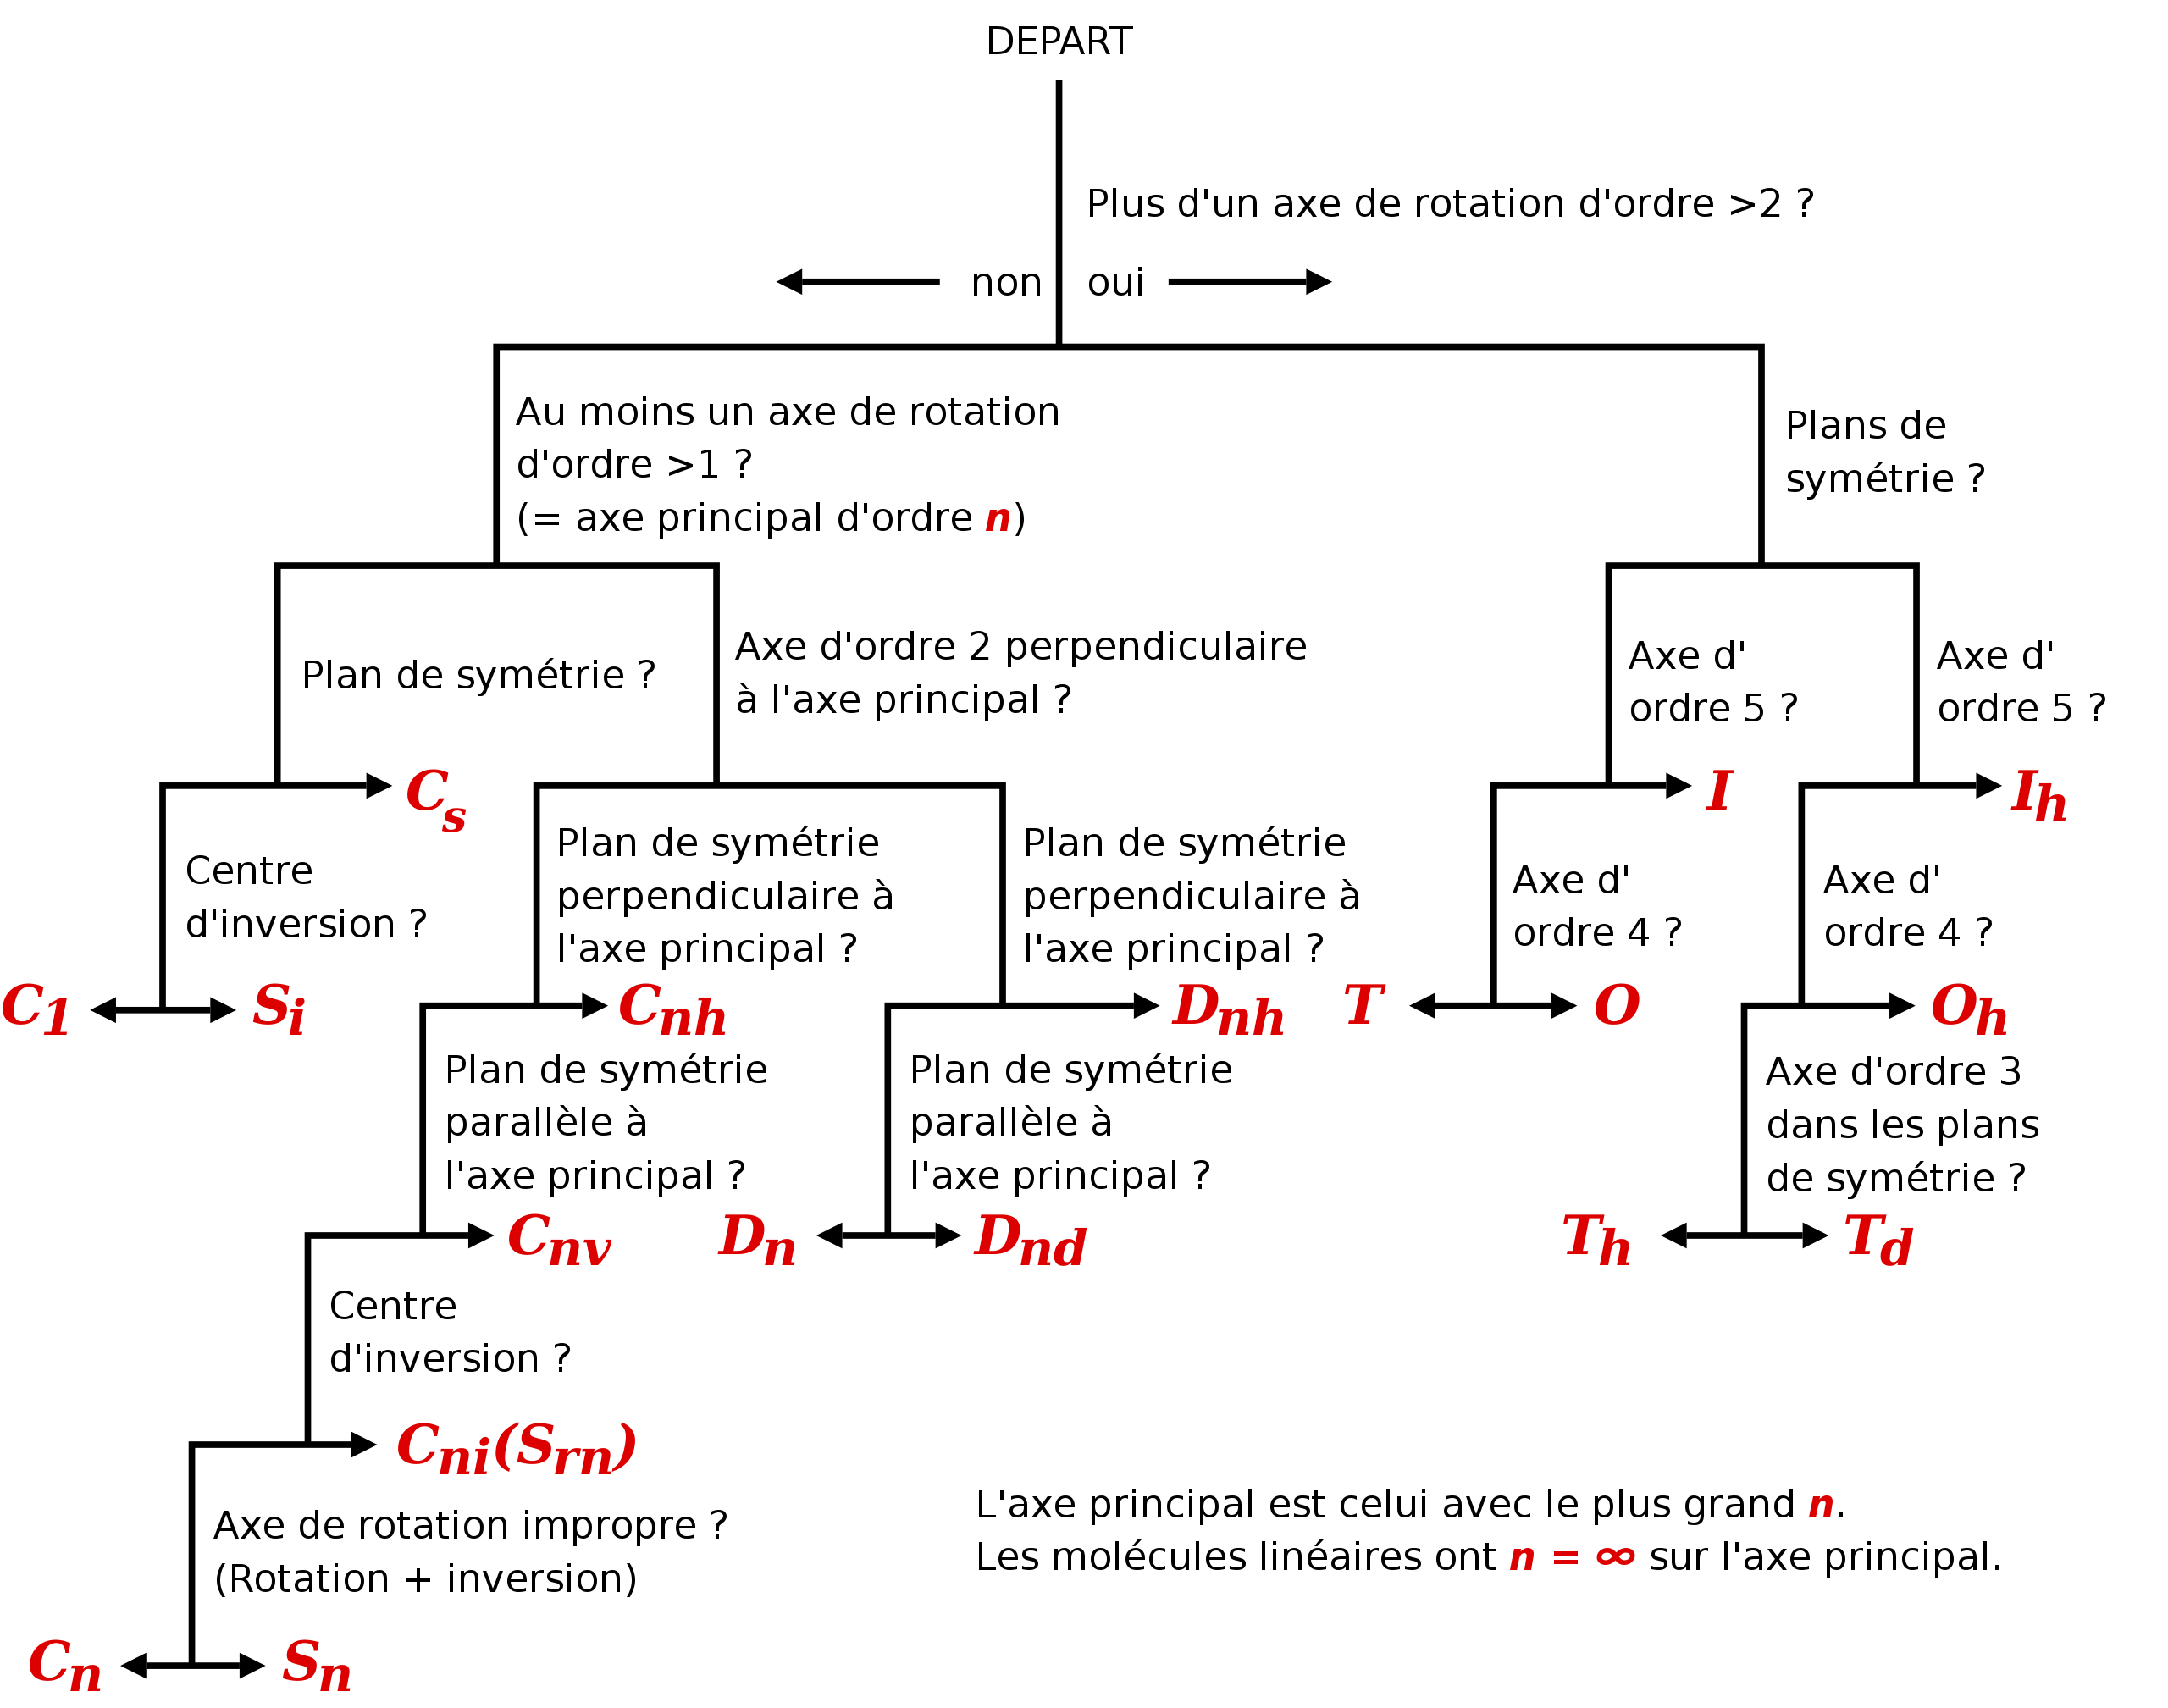
\includegraphics[scale=0.15]{groupe_chimie.png}
    \caption{群论与化学(图片源自法语wiki)}
    \label{myref:groupechimie}
  \end{figure}
  \section{分子对称性和对称群}
  \section{群的表示}
  \section{对称性匹配的线性组合}
  \section{分子轨道理论}
  \section{配体场理论}
  \chapter{概率与位势\\ Probabilités et potentiels}  
  \chapter{场论\\ Théorie des Champs} 
  \chapter{电磁场\\Champs Électromagnétiques}
  \chapter{引力场\\ Champ Gravitationnel}
  \chapter{流体场\\Champs de Fluides}
    \section{理想流体}
    \section{实际流体}
    \section{层流与湍流}
    \section{流体边界层}




  \part{附录 Annexe}
  \appendix
  \chapter{函数表 Table de fonction}
  \section{积分函数表 }
  \section{Fourier变换函数表 }
  \section{Laplace变换函数表 }
  \chapter{三段论 Syllogisme}
  \chapter{证明方法 Méthode de démonstration}
  \chapter{代码 Code}

  \printindex
\end{document}

